%%
%% This is file `thesis-ex.tex',
%% generated with the docstrip utility.
%%
%% The original source files were:
%%
%% uiucthesis2009.dtx  (with options: `example')
%%
\def\fileversion{v2.25} \def\filedate{2016/9/21}
%% Package and Class "uiucthesis2009" for use with LaTeX2e.
\documentclass[edeposit,fullpage]{uiucthesis2009}

%%%%%%%%%%%%%%%%%%%%%%%%%%%%%%%%%%%%%%%%%%%%%%%%%%%%%%%%%%%%%%%%%%%%%% packages
\usepackage[super]{nth}
\usepackage{empheq, amsfonts, amsmath, amsthm, multirow, amssymb, bm, dsfont}
\usepackage{siunitx, nicefrac, microtype, graphicx, epstopdf, color, url}
\usepackage{subcaption, balance, expl3, times, helvet, courier}
\usepackage[super]{nth}
\usepackage[linesnumbered,ruled,vlined]{algorithm2e}
\usepackage[none]{hyphenat}
\usepackage[colorlinks,
           linkcolor=red,
           anchorcolor=green,
           citecolor=blue
           ]{hyperref}
\usepackage[round,authoryear,sort]{natbib}
\usepackage[toc,page]{appendix}
\usepackage{cleveref}
% \usepackage[font=small,labelfont=bf,margin=\parindent,
%             tableposition=top]{caption} % not compatible with aaai
%%%%%%%%%%%%%%%%%%%%%%%%%%%%%%%%%%%%%%%%%%%%%%%%%%%%%%%%%%%%%%%%%%%%%%%%%% math
\renewcommand{\P}{\mathrm{P}}
\newcommand{\E}{\mathbf{E}}
\newcommand{\entropy}{\mathbf{H}}
\newcommand{\var}{\mathbf{var}}
\newcommand{\std}{\mathbf{std}}
\newcommand{\cov}{\mathbf{cov}}
\renewcommand{\d}{\textrm{d}}
\newcommand{\subjto}{\mbox{subject to}}
\newcommand{\NA}{---}
\newcommand{\indct}{\mathds{1}}
% \newcommand*{\qed}{\hfill\ensuremath{\square}}
%%%%%%%%%%%%%%%%%%%%%%%%%%%%%%%%%%%%%%%%%%%%%%%%%%%%%%%%%%%%%%%%%%%%%% Theorems
\theoremstyle{plain}
\newtheorem{thm}{Theorem}[section]
\newtheorem{lem}{Lemma}[thm]
\newtheorem{prop}{Proposition}[thm]
\newtheorem{col}{Corollary}[thm]

\theoremstyle{definition}
\newtheorem{dfn}{Definition}[section]
\theoremstyle{remark}
\newtheorem*{remark}{Remark}
%%%%%%%%%%%%%%%%%%%%%%%%%%%%%%%%%%%%%%%%%%%%%%%%%%%%%%%%%%%%%%%%%%%%%%%% \defeq
\makeatletter
\newcommand*{\defeq}{\mathrel{\rlap{%
  \raisebox{0.3ex}{$\m@th\cdot$}}%
  \raisebox{-0.3ex}{$\m@th\cdot$}}%
   =}
\makeatother
%%%%%%%%%%%%%%%%%%%%%%%%%%%%%%%%%%%%%%%%%%%%%%%%%%%%%%% \mylistbegin \mylistend
% \newcommand{\mylistbegin}{ \begin{list}{$\bullet$} {
%   \setlength{\itemsep}{-2pt}
%     %\setlength{\parsep}{0pt}
%     %\setlength{\topsep}{0pt}
%     %\setlength{\partopsep}{0pt}
%     \setlength{\leftmargin}{1em}
%     \setlength{\labelwidth}{1em}
%     \setlength{\labelsep}{0.5em} } }
% \newcommand{\mylistend}{ \end{list} }
%%%%%%%%%%%%%%%%%%%%%%%%%%%%%%%%%%%%%%%%%%%%%%%%%%%%%%%%%%%%%%% \argmin \argmax
\DeclareMathOperator*{\argmin}{arg\,min}
\DeclareMathOperator*{\argmax}{arg\,max}
\DeclareMathOperator*{\Max}{Max}
\DeclareMathOperator*{\Min}{Min}
\DeclareMathOperator*{\maximize}{maximize}
\DeclareMathOperator*{\minimize}{minimize}
\DeclareMathOperator*{\st}{s.t.}
%%%%%%%%%%%%%%%%%%%%%%%%%%%%%%%%%%%%%%%%%%%%%%%%%%% abbrevations eg etal etc ie
\ExplSyntaxOn
\newcommand\latinabbrev[1]{
  \peek_meaning:NTF . { #1\@}
  { \peek_catcode:NTF a { #1.\@ } {#1.\@}}}
\ExplSyntaxOff
\def\eg{\latinabbrev{e.g}}
\def\etal{\latinabbrev{et al}}
\def\etc{\latinabbrev{etc}}
\def\ie{\latinabbrev{i.e}}
%%%%%%%%%%% shared affiliation: http://www.acm.org/sigs/publications/sigfaq#a17
\def\sharedaffiliation{\end{tabular}\newline\begin{tabular}{c}}
  \newcommand{\superscript}[1]{\ensuremath{^{\textrm{#1}}}}
\def\wg{\superscript{\dag}}
\def\wu{\superscript{*}}
%%%%%%%%%%%%%%%%%%%%%%%%%%%%%%%%%%%%%%%%%%%%%%%%%%%%%%%%%%%%%%%%%%% margin note
\newcommand{\fix}{\marginpar{FIX}}
\newcommand{\new}{\marginpar{NEW}}
%%%%%%%%%%%%%%%%%%%%%%%%%%%%%%%%%%%%%%%%%%%%%%%%%%%%%%%%%%%%%%%%%%%%%% citation
\renewcommand{\cite}{\citep}
%%%%%%%%%%%%%%%%%%%%%%%%%%%%%%%%%%%%%%%%%%%%%%%%%%%%%%%%%%%%%%%%%%%%%%%%% Marco
\newcommand{\DCME}{Dual-Clustering Maximum Entropy}
\newcommand{\PLANS}{Phrasal Latent Allocation with Negative Sampling}
\newcommand{\THETA}{\mathbf{\Theta}}
\newcommand{\vw}{\mathbf{w}}
\newcommand{\vx}{\mathbf{x}}
\newcommand{\vh}{\mathbf{h}}
\newcommand{\vhb}{\boldsymbol{\bar{h}}}
\newcommand{\vv}{\mathbf{v}}
\newcommand{\vW}{\mathbf{W}}
\newcommand{\vV}{\mathbf{V}}
\newcommand{\vH}{\mathbf{H}}
\newcommand{\vs}{\mathbf{s}}
\newcommand{\ii}{\mathcal{I}}
\newcommand{\oo}{\mathcal{O}}
\newcommand{\vmu}{\boldsymbol{\mu}}
\newcommand{\valpha}{\boldsymbol{\alpha}}
\newcommand{\cc}{\textrm{{Classification:}}}
\newcommand{\ee}{\textrm{{Embedding:}}}
\newcommand{\nop}[1]{}
\newcommand{\tpp}{\textsc{Tpp}}
\newcommand{\trm}{\textsc{Trm}}
\newcommand{\vect}[1]{\boldsymbol{\mathbf{#1}}}
\newcommand{\wrt}{\emph{w.r.t.}}
\newcommand{\DP}{\mathcal{DP}}
\newcommand{\pss}{\mathcal{SS}}


%%%%%%%%%%%%%%%%%%%%%%%%%%%%%%%%%%%%%%%%%%%%%%%%%%%%%%%%%%%%%%%%%%%%%%%% shrink
% \renewcommand{\baselinestretch}{0.93}

\begin{document}

\title{Probabilistic Latent Variable Models for  \\
  Knowledge Discovery and Optimization}
\author{Xiaolong Wang}
\department{Computer Science}
\schools{B.A., Peking University, 2011}
\phdthesis
\advisor{Chengxiang Zhai}
\degreeyear{2016}
\committee{Professor Chengxiang Zhai, Chair\\
           Professor Jiawei Han\\
           Professor David Forsyth \\
           Professor Angelia Nedich, ASU \\
           Professor Joy Ying Zhang, CMU }
\maketitle

\frontmatter

%% Create an abstract that can also be used for the ProQuest abstract.
%% Note that ProQuest truncates their abstracts at 350 words.
\begin{abstract}

I conduct a systematic study of probabilistic latent variable models (PLVMs)
with applications to knowledge discovery and optimization. Probabilistic
modeling is a principled means to gain insight of data. By assuming that the
observed data are generated from a distribution, we can estimate its density, or
the statistics of our interest, by either Maximum Likelihood Estimation or
Bayesian inference, depending on whether there is a prior distribution for the
parameters of the assumed data distribution.

One of the primary goals of various machine learning/data mining models is to
reveal the underlying knowledge of observed data. A common practice is to
introduce latent variables, which are modeled together with the observations.
Such latent variables compute, for example, the class assignments (labels), the
cluster membership, as well as other unobserved measurements of the data.
Besides, proper exploitation of latent variables facilities the optimization
itself, which leads to computationally efficient inference algorithms.

In this thesis, I describe a range of applications where latent variables can be
leveraged for knowledge discovery and efficient optimization. Works in this
thesis demonstrate that PLVMs are a powerful tool for modelling incomplete
observations. Through incorporating latent variables and assuming that the
observations such as citations, pairwise preferences as well as text are
generated following tractable distributions parametrized by the latent
variables, PLVMs are flexible and effective to discover knowledge in data mining
problems, where the knowledge is mathematically modelled as continuous or
discrete values, distributions or uncertainty. In addition, I also explore the
PLVMs for deriving efficient algorithms. It has been shown that latent variables
can be employed as a means for model reduction or facilitating
computation/sampling of intractable distributions.

Our results lead to algorithms which take advantage of latent variables in
probabilistic models.  We conduct experiments against state-of-the-art models
and empirical evaluation shows that our proposed approaches improve both
learning performance and computational efficiency.

\end{abstract}


%% Create a dedication in italics with no heading, centered vertically
%% on the page.
\begin{dedication}
To My Family.
\end{dedication}

%% Create an Acknowledgements page, many departments require you to
%% include funding support in this.
\chapter*{Acknowledgments}

This project would not have been possible without the support of many people.
Many thanks to my adviser, Chengxiang Zhai, who read my numerous revisions and
helped make some sense of the confusion. Also thanks to my committee members,
Jiawei Han, David Forsyth, and Joy Zhang, who offered guidance and support.  And
finally, thanks to parents, and numerous friends who endured this long process
with me, always offering support and love.

%% The thesis format requires the Table of Contents to come
%% before any other major sections, all of these sections after
%% the Table of Contents must be listed therein (i.e., use \chapter,
%% not \chapter*).  Common sections to have between the Table of
%% Contents and the main text are:
%%
%% List of Tables
%% List of Figures
%% List Symbols and/or Abbreviations
%% etc.

\tableofcontents
\listoftables
\listoffigures

%% Create a List of Abbreviations. The left column
%% is 1 inch wide and left-justified
% \chapter{List of Abbreviations}

% \begin{symbollist*}
% \item[CA] Caffeine Addict.
% \item[CD] Coffee Drinker.
% \end{symbollist*}

%% Create a List of Symbols. The left column
%% is 0.7 inch wide and centered
% \chapter{List of Symbols}

% \begin{symbollist}[0.7in]
% \item[$\tau$] Time taken to drink one cup of coffee.
% \item[$\mu$g] Micrograms (of caffeine, generally).
% \end{symbollist}

\mainmatter

\chapter{Introduction}

The general treatment of data mining and machine learning can be categorized
into two classes: probabilistic and non-probabilistic. For example, in
classification, probabilistic methods include logistic regression, maximum
entropy, and conditional random fields for binary, multi-class, and sequential
prediction respectively; While one of the most well known non-probabilistic
classification methods, support vector machine (or the more general max-margin
methods) is also investigated for binary, multi-class and structure
predictions. In clustering, there are numerous approaches of both and some
examples are mixture models or matrix factorizations. In this thesis, our focus
is the probabilistic model. It has several important advantages: (1)
Probabilistic models assign probabilities instead of real-valued scores to
outcomes (cluster id, class label), and therefore the output is naturally
statistical meaningful.  (2) Maximum likelihood estimation (MLE), or
equivalently, Kullback-Leibler (KL) divergence minimization, is the principled
and generic objective for optimization. For non-probabilistic models, expert
knowledge is required to select the objective function which yields the best
performance.  (3) In Bayesian settings, the prior distribution of model
parameters plays the role of model regularization with Maximum a Posterior (MAP)
or posterior expectation extending MLE. These advantages are very appealing in
both theory and practice. However, it is not the intention of this thesis to
demonstrate that the probabilistic models are superior to non-probabilistic
ones.

Probabilistic latent variable models (PLVMs) have provided a mathematical-based
approach to the statistical modeling of a wide variety of random phenomena which
cannot be explained well by simple distributions, such as binomial, multinomial,
Poisson, and Gaussian, Dirichlet for discrete and continuous distributions
respectively. PLVM assumes that the observed data is accompanied by another
group of ``unobserved'' latent variables. And the distribution of the observed
data is conditioned on the latent variables. Therefore, It is able to model
quite complex distributions through an appropriate choice of its latent
variables to represent accurately the local areas of support of the true
distribution. Computation can be made feasible from the latent variables, as the
latter are usually chosen with a tractable form.

An illustrating example, topic modeling, demonstrates how latent variables can
be used for modeling ``topics.'' A topic is mathematically represented by a
multinomial distribution over words in the vocabulary and the unigram
distribution of a document is regarded as the result of a ``mixture'' of the
topics. Though our observation is merely words in the document, by introducing
the latent variables, namely the topics and the mixture weights of documents,
the semantic relationship of words can be identified to a great extent and the
prominent subject of a document can be revealed as well. For instance, it is
expected that words like ``science'' and ``technology'' would have large
probability in one topic while others like ``baseball'' and ``basketball'' would
in another topic. In computer vision, topic modeling is also applied to the task
of image segmentation where pixels of an image are seen as a mixture of latent
objects.

We devote the rest of this section to illustrate how we can leverage
probabilistic latent variable models for knowledge discovery and optimization.

\section{Latent Variable for Knowledge Discovery}

PLVMs as an extremely flexible method of modeling have been extensively
investigated in knowledge discovery and data mining. In recent decades, from
probabilistic latent semantic indexing, latent Dirichlet allocation, to
Dirichlet process, Indian buffet process, we have witnessed numerous of PLVMs
being proposed and widely applied to varying fields such as natural language
processing, speech recognition, and computer vision. To focus our discussion, we
restrict our analysis to the mixture models, also more known now as topic
modeling in recent literature.

\subsection{Mixture Models --- an Historical Account} The early effort of
studying on mixture models can be dated back to
\citeyear{pearson1896mathematical} when Karl Pearson fitted a mixture of two
normal probability density functions~\cite{pearson1896mathematical} on the
problem of \emph{Breadth of ``Forehead'' of Crabs}. As a pioneering
biostatistician, he has been credited for the finite mixture models and method
of moments among his other contributions. In hindsight, his work also
established the computational (optimization) theory of statistical modeling,
which strikes me as a visionary as it remains a difficult yet interesting
research area and inspires my study on this topic which composes most of this
thesis.

The dataset on which Pearson modelled consisted of measurement on the ratio of
forehead width to the body length of 1000 crabs sampled at the Bay of Naples by
zoologist W.F.R. Weldon. Weldon analyzed the histogram of the observations,
which is plotted in Figure~\ref{fig::pearson-crab}, along with a normal
distribution fitted using Maximum Likelihood~(see the solid blue line). However,
\citet{weldon1893certain} speculated that the asymmetry in the histogram, ``a
well-marked deviation from this normal shape,'' could be resulted from a
hypothesis that ``the units grouped together in the measured material are not
really homogeneous.'' To validate whether the population of crabs was evolving
toward two subspecies, he turned to his colleague Pearson for help on
mathematics.

\begin{figure}[ht!]
  \centering
  \begin{subfigure}[b]{0.95\textwidth}
  \centering
  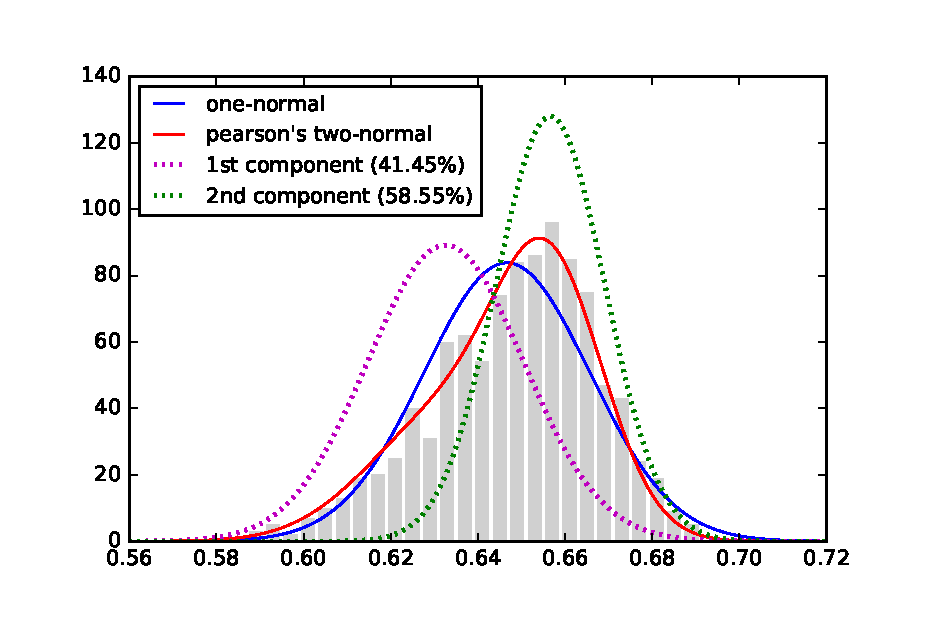
\includegraphics[width=0.8\linewidth]{figures/pearson-crab.eps}
  \caption{In this plot, the bar chart of the observations from Weldon is shown
    in grey. The blue solid line shows the single normal distribution fitting
    the data using Maximum Likelihood; And the solid line in red plots the
    mixture model of two normals distributions derived by Pearson using moment
    matching where its two components are also displayed in green and purple
    dotted lines.}
  \label{fig::pearson-crab}
  \end{subfigure}
  ~
  \begin{subfigure}[b]{0.95\textwidth}
  \centering
  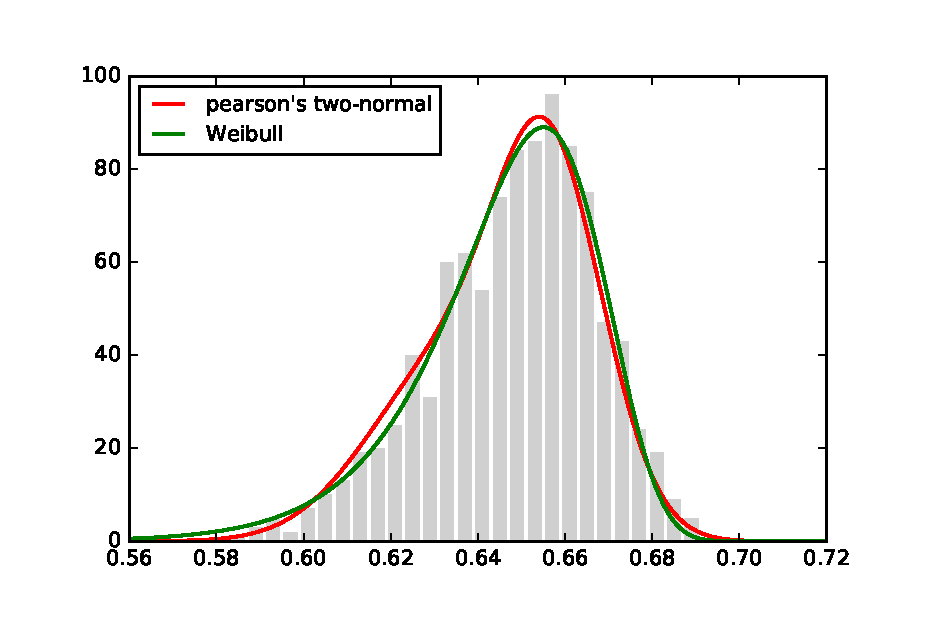
\includegraphics[width=0.8\linewidth]{figures/pearson-crab-weibull.eps}
  \caption{Comparison between the Pearson's mixture of two normals and a single
  Weibull distribution. Pearson's mixture model provides a better fitting at the
  mode of empirical distribution. Note that the form of density function of
  Weibull distribution is much more complicated than that of normal distribution
  and it requires numeric means to estimate the parameters.}
  \label{fig::pearson-crab-weibull}
  \end{subfigure}
  \caption{Pearson's Mixture of Two Normals on ``Breadth of Forehead of Crabs''}
\end{figure}

Pearson used two normal distributions to fit the observations. To estimate the
parameters, namely, the means ($\mu_1, \mu_2$) and standard-variance ($\sigma_1,
\sigma_2$) of the two normal distributions as well as the proportions ($\pi_1,
\pi_2$) of the two components, Pearson followed the method of moments (which
was also introduced by himself in 1894). Though moment matching is superseded
by Fisher's method of maximum likelihood~\cite{pfanzagl1994parametric} in
nowadays classic statistical modelling, it was a numerically simpler approach
in most cases. However, the calculation was still formidable and daunting at
the time without the aid of computer or other machinery of any kind.
Mathematically, the problem involves five parameters $\mu_1, \mu_2, \sigma_1,
\sigma_2$ and $\pi_1$ (we can obtain $\pi_2 = 1 - \pi_1$) and to find a
solution the parameters need to ensure that the mixture matches on the first
five moments. Pearson derived a ninth degree polynomial (nonic) and two
candidate real roots are found. He finally chose the solution on the basis of
agreement with the sixth moment. In Figure~\ref{fig::pearson-crab}, the dashed
curve in red shows Pearson's mixture and its two components are displayed in
purple and green dashed lines. Clearly, the mixture is skewed and better fits
the histogram. And indeed, two subspecies are identified which verifies the
hypothesis of Weldon.

It is quite an advanced idea to leverage latent variables for statistical
modeling at that time. Otherwise fitting the asymmetric observations would
involve a much more complicated distribution. In fact, we can also fit the data
with a skewed Weibull distribution, the parameter of which are nevertheless
computational difficult to estimate (The Maximum Likelihood estimator for the
shape parameter is the solution to the equation $\frac{1}{k} =
\frac{\sum_{i=1}^N (x_i^k\log x_i - x_N^k \log x_N) }{\sum_{i=1}^N (x_i^k -
x_N^k)}- \frac{1}{N}\sum\limits_{i=1}^N \log x_i$, and numeric methods, which
were very primitive at the time of late 19th century, is required.) Therefore
Weibull distribution was not a practical option for fitting the data without the
aid of computers. In Figure~\ref{fig::pearson-crab-weibull}, we compare the
Peason's mixture of two normals with one single Weibull distribution fitting the
data using Maximum Likelihood. The difference between the two curves is not
significant. However, Pearson's result seems to fit better at the mode around
$0.66$.

\subsection{Mixture Models --- Development of EM algorithm}

Although solving the mixture model with the method of moments is a very
laborious task and performing the necessary calculation is even more
heroic~\cite{mclachlan2004finite}, it does not always yield the optimal solution
in the statistical sense. The maximum likelihood approach, however, possesses
superior statistical property as it tries to place higher probability close to
the observed data and are more often unbiased. With the development of computer
and optimization in the last century, modern statistical modeling is able to
utilize numeric algorithms to solve Maximum Likelihood Estimator (MLE).  Among
the different optimization methods, Expectation-Maximization (EM)
algorithm~\cite{dempster1977maximum} has greatly stimulated interest in the use
of mixture models as well as other PLVMs. Several reasons can be accounted for
the popularisation of EM algorithm: (1) It is generally easy to implement the
algorithm and it has virtually no parameters to tune, as compared to, for
example, gradient descent, where a carefully selected learning step is required
to ensure fast training; (2) It usually does not need any special treatment to
handle the constraints of the model. For example, in the normal mixture problem,
the standard-variance of a component normal is always positive and in EM
algorithm and this is naturally satisfied since it is computed as the empirical
standard-variance of the ``generated'' completed data from the posterior
distribution; (3) EM is a flexible family of approaches where the variational
distribution in the expectation step can be simplified (or constrained) for the
purpose of computation efficiency (e.g. mean-field EM) and the maximization step
can also be substituted by an ascend step. We leave the details of EM algorithm
in Chapter~\ref{sec::bg-em}.  In this section, we provide a brief comparison
between EM algorithm and Pearson's method of moments and show how we can
improve Pearson's result by EM algorithm.

\begin{figure}[ht!]
  \centering
  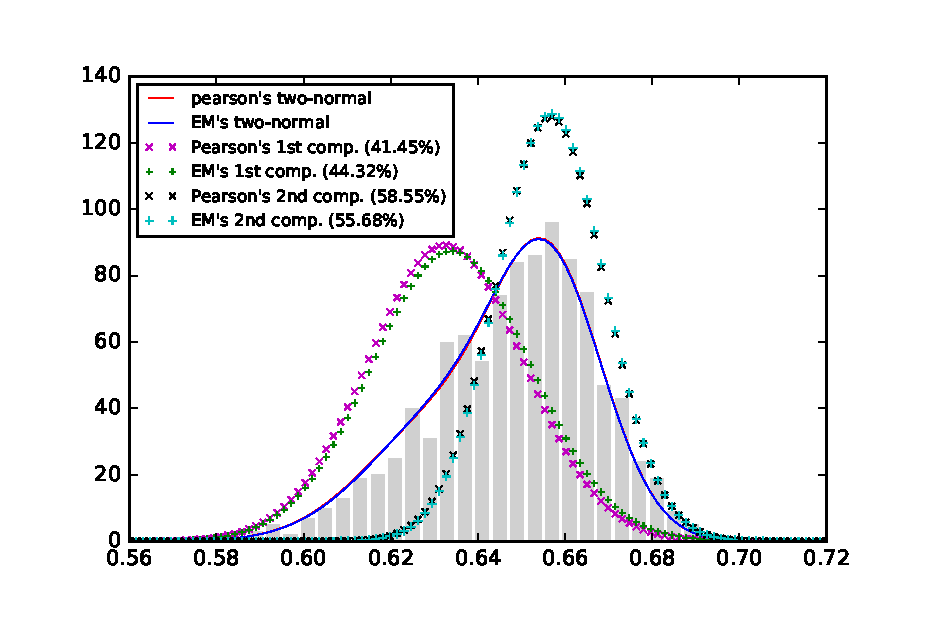
\includegraphics[width=0.8\linewidth]{figures/pearson-crab-em.eps}
  \caption{Comparison of the mixture model of two normals between Pearson's
  approach and EM algorithm. The two mixture models are very close to each
  other showing that the moment-matching method of Pearson obtains a near
  optimal likelihood.}
  \label{fig::pearson-crab-em}
\end{figure}

We plot the curves of the mixture models of the two methods as well as their
components in Figure~\ref{fig::pearson-crab-em}. The results are almost
identical. To assess the quality of the model quantitatively, Pearson used the
Chi-square test~\cite{pearson1900x} which he proposed to examine if the observed
data is indeed from the model. We follow his practice and report the result in
Table~\ref{tab::pearson-em-crab}.

\begin{table}[h]
  \centering
  \caption{Pearson's Chi-square test and p-Value for a single normal model, a
    single Weibull model, and the two normal mixture model of Pearson and EM
    algorithm in the ``Breadth of Forehead of Crabs'' problem. For the normal
    models, we also include the model parameters.}
  \label{tab::pearson-em-crab}
  \setlength\tabcolsep{5pt}
  \begin{tabular}{c|cccccc|c|cc}
    Method & $\mu_1$ & $\mu_2$ & $\sigma_1$ & $\sigma_2$ & $\pi_1$ & $\pi_2$
           & freedom & Chi-square & p value \\ \hline \hline
    Single Normal & 0.6466 & \NA & 0.0190 & \NA & 1 & \NA & 2 & 71.6836 &
    \num{2.157e-6} \\
    Single Weibull & \NA & \NA & \NA & \NA & \NA & \NA &
    2 & 28.3841 & 0.2904 \\
    Pearson & 0.6326 & 0.6566 & 0.0179 & 0.0125 & 0.4145 & 0.5855 &
    5 & 21.0342 & 0.5186 \\
    EM & 0.6339 & 0.6568 & 0.0182 & 0.0124 & 0.4432 & 0.5568 &
    5 & 20.8438 & 0.5304 \\
    %\hline \hline
  \end{tabular}
\end{table}

As expected, we see that the EM algorithm results in the smallest Pearson's
Chi-square. In less mathematical terms, the observed data is distributed more
close to the model given by the EM algorithm. In addition, the p-values in the
significant test show that it is more certain that the data is sampled from the
mixture normal of EM algorithm. To an extent, the assessment on the Weldon's
crab dataset justifies the use of EM algorithm to solve MLE in applications of
mixture modeling.

% EM:         (statistic=20.843800910788627, pvalue=0.53040874121547321)
% Pearson:    (statistic=21.034210586530026, pvalue=0.51862468978687204)
% uni-normal: (statistic=71.683615393997414, pvalue=2.1571531876646807e-06)
% Pearson:    (0.6326, 0.6566, 0.0179, 0.0125, 0.4145, 0.5855)
% EM:         (0.6339, 0.6568, 0.0182, 0.0124, 0.4432, 0.5568)
% Weibull:    (statistic=28.384054004025337, pvalue=0.29047889023764795)

\subsection{From Mixture Models to Topic Modeling}

Since the late of 1990s, the study on document understanding has witnessed a new
rising approach of PLVMs which is often referred as topic modeling. The first
well recognized topic modeling method, probabilistic latent semantic
indexing~(PLSI)~\cite{hofmann1999probabilistic}, is simple yet effective.
Essentially it sees the distribution $w_d$ of unigrams for a document $d$ as a
$K$-mixture of multinomial distributions $\beta_1, \dots, \beta_K$ with
proportions $\theta_{d, 1}, \dots, \theta_{d, k}$. Those $\beta_K$ are referred
as ``topics'' because the words of large probabilities in a component are often
semantically related. In addition, the topic weights $\theta_d$ of a document
provides a short summary of the documents.  Computationally, $\theta_d$ has a
much lower dimensionality than $w_d$ and thus can be leveraged as a (part of)
feature vector in tasks such as document classification or clustering. Moreover,
$\theta_d$ is semantically meaningful as similarity of $\theta_d$ correlates
with the subject of the documents, which can be greatly useful in document
understanding.

Later development of topic modeling includes numerous works which are beyond of
the focus in this thesis. In terms of modeling the latent variables, there are
two aspects of milestone progress that are worth a brief overview: the Bayesian
inference and nonparametric statistics. The early effort promoting the Bayesian
nonparametrics and advocating the theoretical formalization of topic modeling,
specifically, the analysis on random processes of exchangeable
partitions~\cite{pitman1995exchangeable}, are the lectures taught by
\citeauthor{pitman2002combinatorial} at Berkeley in Spring
\citeyear{pitman2002combinatorial}. Many of David Blei's later
works~\cite{blei2009topic,blei2003latent,blei2010nested} are immediate fruit of
the lectures and readers interested in a principle introduction on this topic
should refer to the lecture notes~\cite{pitman2002combinatorial} and the
references therein.

\emph{Bayesian inference} departs from the tradition MLE framework. It assumes a
prior distribution on latent variables parametrized by the
\emph{hyperparameters}. The advantages of introducing a prior on latent
variables are mainly two folds and we show them using the Latent Dirichlet
Allocation~(LDA)~\cite{blei2003latent} as an example: (1) It enables user to
incorporate human knowledge about the latent variables into modeling. In
document understanding, the word distribution of a topic as well as the
proportion of topics for a document are naturally sparse. LDA encourages such
behavior by adding a Dirichlet prior. (2) By selecting the form of prior
carefully, the prior and posterior can be in the same (with different parameters
though). Such conjugate prior-posterior pairs are computational beneficial in
both Gibbs sampling as well as variational inference. LDA chooses Dirichlet as
the conjugate prior to multinomial distribution. Another significant difference
between Bayesian inference and MLE is the estimation method. There are two major
estimation methods of the latent variables in Bayesian setting which are
Bayesian estimator (posterior expectation) and maximum a posterior (MAP). The
first computes the posterior expectation of the latent variables given the
observed data while the second selects the value with the maximal probability in
the posterior distribution, which can be viewed as an extension of the MLE
method. In the context of topic modeling, it has been noticed that Bayesian
estimator is more popular than the alternatives. The major criticism of MAP is
the fact that it is not very representative of Bayesian methods in general
because it is still a point estimates in nature. Specifically in topic modeling,
it is common that the posterior distribution of the latent variables are in fact
multi-modal and therefore it is computational infeasible (or even intractable)
to calculate MAP due to the non-convex nature of the problem.

\emph{Nonparametric statistics} aims to model the data with possibly infinite
number of latent variables. In topic modeling, it means that one can model
infinite large number of topics or words in the vocabulary. Although in practice
it does not seem to be useful immediately since there is always a finite
upper-bound for these quantities, it relies on expert knowledge to appropriately
select the values. Nonparametric statistics are most powerful to learn the
number of latent variables that are adequately large to explain the data by
using random processes. Random processes are extensively studied in recent
literature, as surveyed in \cite{hajek2015random}, including Gaussian
process~\cite{rasmussen2006gaussian}, Dirichlet process~\cite{teh2011dirichlet},
Indian buffet process~\cite{ghahramani2005infinite}, and hierarchical
processes~\cite{teh2012hierarchical,griffiths2004hierarchical,blei2010nested},
just to name a few. Mathematically, to model the latent variables from possibly
infinite number of choices, the nonparametric approach assumes a random process
as prior. Computationally, there are mainly two strategies, Gibbs sampling and
truncated variational inference, to estimate the posterior distribution of the
possibly infinite number of latent variables. Gibbs sampling takes advantage of
the fact that the prior process usually yields a simple prediction rule of one
latent variable given all others. For example, in Dirichlet process, using the
notion of Chinese restaurant process~\cite{pitman2002combinatorial}, the
probability of a latent variable choosing an existing or a new value is
proportional to the sum of a hyperparameter $\alpha$ and the number of other
latent variables of the same value:

\begin{eqnarray}
  \P_{CRP}(z_i = k | z_1, \dots, z_{i-1}, z_{i+1}, \dots, z_N)
    \propto
      \begin{cases}
        \alpha + \sum\limits_{j = 1, j \neq i}^N \indct( z_j = k )
        & \text{if $k < K$} \\
        \alpha
        & \text{if $k = K + 1$}
      \end{cases} \\
\end{eqnarray}
Where it is supposed that the value of $z_j, j \neq i$ is choosing from $1,
\dots, K$  and for any $k < K$ the support is nonempty. Therefore it is feasible
to investigate sampling methods for inference. While alternatively, another
strategy for estimation is to approximate the possibly infinite posterior with a
finite approximation. For the Dirichlet Process (as well as the generalized
Pitman-Yor two-parameter process~\cite{pitman1997two}), the truncating
approximation is based on a stick-breaking~\cite{ishwaran2011gibbs}
interpretation. It views the process as breaking a stick with the proportion as
a sample from a Beta distribution and the truncation stops the breaking after
there is a predefined number of sticks generated. Both of the above two
strategies have advantages as Gibbs sampling does not need to truncate the size
of latent variables by a finite number while the truncated variational inference
is generally more computational efficient. However, as shown in
\cite{wang2012truncation}, it is possible to combine the two ideas together by
performing the E-step in the variational EM via sampling.

\section{Latent Variable for Optimization}

Previous research such as topic modeling mainly incorporates the latent
variables for the purpose of knowledge discovery. Another motivation to use
latent variable models is efficient computation. In previous discussion, we have
already witnessed that by introducing latent variable, the mixture model of
Pearson is much more easier to compute than that of Weibull distribution.
However, contemporary effort in the direction of leveraging PLVMs for efficient
computation was less explored. In one of the recent work by the author,
Dual-Clustering Maximum Entropy (DCME)~\cite{wang2016dcme}, it demonstrats that
the PLVM is an effective means to improve the optimization efficiency.

Maximum Entropy is an classic approach in classification as well as word
embedding. However, it becomes computationally challenging when the number of
classes or the vocabulary size is large. DCME approaches the problem by
optimizing ME in its primal-dual form. The key insight is to introduce a latent
cluster assignment for each training instance and assume that the dual variables
of an instance are determined by the corresponding latent assignment. As an
initial investigation, we use the latent variables in a much simpler manner than
the mixture models. Specifically, we restrict the latent variable distributed as
a Kronecker delta which has support only on a single value, as contrast to the
case of mixture model where the latent variable is distributed as a more general
multinomial. DCME naturally leads to an approximation of the dual variables
which can be computed by a K-means like clustering. In addition, it also enables
a efficient online-offline computation scheme whose computation complexity does
not depends on the number of classes nor the vocabulary size. And the empirical
study demonstrated that DCME outperforms other state-of-the-art approaches.

\section{Overview of This Thesis}

In the rest of this thesis, we will discuss in detail on the PLVMs.
Specifically,  In chapter~\ref{chp::bg}, we briefly discuss a few key
mathematics that can greatly facilitate the understanding of the PLVMs.

Next, we will show two scenarios where PLVMs are applied in data mining for
knowledge discover.

The first work analyzes the citations of
literatures~\cite{wang2013understanding}. Understanding how research themes
evolve over time in a research community is useful in many ways (e.g., revealing
important milestones and discovering emerging major research trends).  In this
study, we propose a novel way of analyzing literature citation to explore the
research topics and the theme evolution by modeling article citation relations
with a probabilistic generative model.  The key idea is to represent a research
paper by a ``bag of citations'' and model such a ``citation document'' with a
probabilistic topic model.  We explore the extension of a particular topic
model, i.e., Latent Dirichlet Allocation~(LDA), for citation analysis, and show
that such a Citation-LDA can facilitate discovering of individual research
topics as well as the theme evolution from multiple related topics, both of
which in turn lead to the construction of evolution graphs for characterizing
research themes.  We test the proposed citation-LDA on two datasets: the ACL
Anthology Network~(AAN) of natural language research literatures and PubMed
Central~(PMC) archive of biomedical and life sciences literatures, and
demonstrate that Citation-LDA can effectively discover the evolution of research
themes, with better formed topics than (conventional) Content-LDA.

The second work explores PLVMs in a crowdsourcing setting~\cite{wang2016tpp}.
Crowdsourcing services make it possible to collect huge amount of annotations
from less trained crowd workers in an inexpensive and efficient manner.
However, unlike making binary or pairwise judgements, labeling complex
structures such as ranked lists by crowd workers is subject to large variance
and low efficiency, mainly due to the huge labeling space and the annotators'
non-expert nature. Yet ranked lists offer the most informative knowledge for
training and testing in various data mining and information retrieval tasks such
as \textit{learning to rank}.  In this paper, we propose a novel generative
model called ``Thurstonian Pairwise Preference'' (\textsc{Tpp}) to infer the
true ranked list out of a collection of crowdsourced pairwise annotations.  The
key challenges that \textsc{Tpp} addresses are to resolve the inevitable
incompleteness and inconsistency of judgements, as well as to model variable
query difficulty and different labeling quality resulting from workers' domain
expertise and truthfulness.  Experimental results on both synthetic and
real-world datasets demonstrate that \textsc{Tpp} can effectively bind pairwise
preferences of the crowd into rankings and substantially outperforms previously
published methods.

In addition, as hinted before, another aspect of PLVMs is to improve the
efficiency of optimization. To this end, we devote another chapter to discuss
the study of Dual-Clustering Maximum Entropy~\cite{wang2016dcme}.  Maximum
Entropy (ME), as a general-purpose machine learning model, has been successfully
applied to various fields such as text mining and natural language processing.
It has been used as a classification technique and recently also applied to
learn word embedding. ME establishes a distribution of the exponential form over
items (classes/words). When training such a model, learning efficiency is
guaranteed by \emph{globally} updating the entire set of model parameters
associated with \emph{all} items at \emph{each} training instance. This creates
a significant computational challenge when the number of items is large. To
achieve learning efficiency with affordable computational cost, we propose an
approach named Dual-Clustering Maximum Entropy (DCME).  Exploiting the
primal-dual form of ME, it conducts clustering in the dual space and
approximates each dual distribution by the corresponding cluster center.  This
naturally enables a hybrid online-offline optimization algorithm whose time
complexity per instance only scales as the product of the feature/word vector
dimensionality and the cluster number. Experimental studies on text
classification and word embedding learning demonstrate that DCME effectively
strikes a balance between training speed and model quality, substantially
outperforming state-of-the-art methods.


\section{Background}

As aforementioned, three are three necessary ingredient to develop the PLANS. In
this section, we formally discuss them in detail.

\subsection{Phrasal Allocation as Transient Chinese Restaurant Process (tCRP)}

Dirichlet process is a stochastic process used in Bayesian nonparametrics, which
extends the Dirichlet distribution, to model the discrete count observations
over an infinite number of outcomes. It has a nice interpretation, namely the
Chinese restaurant process~(CRP), which provides a intuitive metaphor: Suppose
that there is an infinite number of tables in a Chinese restaurant, and the
first customer enters the restaurant to sit at the first table. The second
customer enters and decides either to sit with the first customer or alone at a
new table. In general, the $n+1$-th customer either joins an already occupied
table indexed by $k$ with probability proportional to the number of customers
already sitting there, or sits at a new table with probability proportional to a
hyperparameter $\alpha$.

We adopt CRP for phrasal allocation and assume that there is a table for each
phrase and customers correspond to occurrences of phrases in the dataset.
However, CRP posits two difficulties to properly model the phrasal allocation:
(1). For a stream of words $\dots, w_{t_1}, w_t, w_{t+1}, \dots$ in the dataset,
it is only reasonable for $w_t$ to be enclosed by phrases of the form $\langle
w_b, \dots, w_e \rangle$ where $b \le t \le e$ and $t - b$, $e - t$ are small.
Thus when $w_t$ enters the restaurants, its choice of seating is be limited; and
(2).  When learning on a corpus of very large size or stream, it is unrealistic
to run the CRP (sampling) over the data (enough epochs until convergence). In
plain words, it is unappealing that the number of accommodated tables as well as
seated customers to grow constantly over time. To this end, transient Chinese
restaurant process~(tCRP) is proposed.

\begin{algorithm}[h!]
\caption{Transient Chinese Restaurant Process}\label{alg::tcrp}
  \SetAlgoNoLine
  \For{$t = 1, 2, \dots$}{
    $\mathcal{P}_t \leftarrow
      \left\{ \langle w_b, \dots, b_e \rangle :
        b \le t \le e ~\text{and}~ e - b \le L \right\}$\;
    $\mathcal{V}_t \leftarrow \text{existing tables in the restaurant}$\;
    $\mathcal{A}_t \leftarrow \mathcal{P}_t \setminus \mathcal{V}_t$\;
    Let $\mathcal{N}(p_k),\, (k = 1, \dots, \left\vert\mathcal{V}_t\right\vert)$
      be the number of customers sitting at the table of phrase $p_k$\;
    \textbf{Sample} $k^* \in \{1, \dots, \left\vert\mathcal{V}_t\right\vert\}$
      with probability:\\ {
       \Indp
       \uIf{$k^* \in \mathcal{A}_t$  }{
         $\P(k^*) \propto \frac{\alpha}{ \left\vert\mathcal{A}_t\right\vert}$\;
        }
       \uElse {
         $\P(k^*) \propto \mathcal{N}(p_{k^*})$\;
       }
     }
    \uIf{current block is completed}{
      \textbf{Shrink} for each phrase $p$:
        $\mathcal{N}(p) \leftarrow \beta \mathcal{N}(p)$\;
      \textbf{Sort} phrases by $\mathcal{N}(p)$\;
      \textbf{Prune} by retaining only the top $V$ phrases\;
    }
  }
\end{algorithm}

The first difference between tCRP and CRP is that the choice of tables for a
customer $w_t$ (occurrence of word) in tCRP is restricted to those corresponding
to the possible phrases $\langle w_b, \dots, w_e \rangle$ where $b \le t \le e$
and $e - b \le L$. It only considers phrases include the word $w_t$ and has the
length no longer than $L$, which is a parameter given by the user.  tCRP assigns
the probability for a customer to sit at an existing table proportional to the
number of customers already there. However, to sit at a new table, the
probability is proportional to the hyperparameter $\alpha$ divided by the number
of possible new tables available to the customer, which is different from the
setting of CRP.

Another significant feature of tCRP is that it allows customers to leave the
restaurant when they finish ``dining''. Specifically, after customers in a block
of data are seated, customers in tCRP choose to leave with a probability
$\beta$. It has a ``aging'' effect since the for a customer to stay in the
restaurant after $i$ data block, the probability is $(1 - \beta)^i$, which
decreases exponentially with $i$. In addition, the restaurants will sort the
tables by the number of customers and only retain the top $V$ tables. In this
way, we maintain an affordable number tables (phrases) in tCRP.

The above procedures of tCRP is summarized in \Cref{alg::tcrp}.

\subsection{Phrase Embedding Learning with Negative Sampling}

The second ingredient in PLANS is negative sampling for estimating the phrase
embeddings. Suppose that given a context phrase $p_i$,
the maximum likelihood model would compute the probability of predicting the
target phrase $p_k$ as:

\begin{equation}
  \P(p_k | p_i) =
    \frac{\exp(\vv_k^T \vh_i)}{\sum\limits_{j=1}^V \exp(\vv_j^T \vh_i)}
\end{equation}

where the $\vv_k$ and $\vh_i$ are the \emph{output} and \emph{input} vector for
phrase $p_k$ and $p_i$, respectively.  We adopt the Skimgram model to substitute
this probability with a scoring function in the similar spirit of the
noise-contrastive estimation approach, and now we have:

\begin{equation}
  \mathcal{S}(p_k | p_i) =
  \log\sigma(\vv_k^T \vh_i) +
  \sum\limits_{l=1}^Q \log(1 - \sigma\big(\vv_{\mathcal{P}_l}^T \vh_i)\big)
\end{equation}

where in Skipgram as well as noise-contrastive estimation, a noisy distribution
is assumed to be easy sampled from, and $\{\mathcal{P}_l\}$ are samples from the
noisy distribution. Although using the score $\mathcal{S}$ instead of the
probability no longer preserves the statistical justification, it is
computationally efficient and performs well in practice.

Combining the negative sampling with the tCRP discussed earlier it is now
possible to jointly discover the phrase and learn the embeddings. Given a
context word $w_c$ and a target word $w_t$. The posterior probability to sample
a phrase $p_c$ for $w_c$ is thus proportional to:

\begin{equation}
  \P(p_c | w_c, w_t) \propto \P_{tCRP}(p_c | w_c) \mathcal{S}(w_t | p_c)
\end{equation}

Another strategy is to sample phrases for both context and target words.
Specifically, we will sample not only the context phrase but also the target
phrase. However, the sampling of the two phrases is coupled, and thus
computationally difficult:

\begin{align}
  \P(p_c | w_c, w_t, p_t) &\propto \P_{tCRP}(p_c | w_c)  \mathcal{S}(p_t | p_c)
    \\
  \P(p_t | w_c, w_t, p_c) &\propto \P_{tCRP}(p_t | w_t)  \mathcal{S}(p_t | p_c)
\end{align}

\subsection{Simulated Annealing}

With the trained data increasing, PLANS is more and more certain about the
language structure and the phrasal allocation. Therefore, it is appealing to
decrease the stochastic behavior of sampling. Another motivation is to stabilize
the phrase set when approaching the end of training. Intuitively speaking, this
is the same idea of decreasing the learning step size for gradient descent. To
this end, we investigate simulated annealing~(SA) in PLANS, which modifies the
posterior probability for sampling with a temperature $T_t$

\begin{equation}
  \P_{SA}(p_c | w_c, w_t) \propto \P^{1/T_t}(p_c | w_c, w_t)
\end{equation}

where $\lim_{t\rightarrow \infty} T_t = 0$. Under weak regularity assumption, it
is easy to see that the probability in SA density concentrates on the mode of
original distribution. In other words, the phrase with the maximum posterior
probability will be deterministically selected.

the temperature function, $T_t$, is yet to be specified. There are many
annealing schedule that we can explore. The \emph{geometric cooling}, where the
temperature is computed suing:

\begin{equation}
  T_t = \gamma^t T_0
\end{equation}

where $0 < \gamma < 1$ is the cooling rate, which usually takes value between
0.8 to 0.99~\cite{yuan2004annealed}. The geometric cooling is widely used for
its quick cooling and convergence. In our work, we set $\gamma = 0.99$.



% They either learn the
% phrase embedding phrases by the directly~\cite{yin2014exploration}; or a
% composition function which computes the phrase embedding from the embedding of
% the constituent
% words~\cite{yu2015learning,le2015compositional,irsoy2014deep,socher2011dynamic,
% baroni2010nouns,zhao2015phrase,levy2014dependency}. Another category of study
% focuses on the inference of the structure in an supervised manner
% manner~\cite{socher2013parsing}, which is different from some of the first
% category in the aspect that a structure decoding model is jointly learned.
% % or factorization methods~\cite{huang2015convolutional,van2013tensor,yu2016embedding}


\chapter{Understanding the Evolution of Research Themes:
  a Probabilistic Generative Model for Citations}\label{chp::clda}
\section{Introduction}

In this chapter, I demonstrate that by modeling literature citations as
observations of a generative model with latent variables, research topics as
well as evolution themes of research can be identified and described inactively.
It exemplifies that PLVM is an effective means for knowledge discovery in data
mining problems. Though we use literature citation as the test bed for PLVM, the
method presented here can be easily applied to any general network data as well.

How to leverage information technologies to improve the  productivity of
scientific research is a highly important challenge with clearly huge impact on
the society. One bottleneck in research productivity is that as a research
community grows, it would be increasingly difficult for researchers to see the
complete picture of how a field has been evolving, given the fact that large
volume new literatures are written based on previous works. Junior researchers
can often get lost in the overwhelming amount of related papers. Researchers who
seek to shift to a new topic may spend lots of time preparing a reading list on
his/her own. All these clearly hinder the progress of scientific research, and
it would be highly beneficial to develop mining techniques to help researchers
more easily and more efficiently  understand research themes in scientific
literature.  In general, two aspects of analysis are needed for understanding
research themes: First, we need to analyze \emph{each research topic} to answer
the following questions: Which papers are the milestone papers that best
represent a topic and how to quantify their impact?  When did the topic become
popular and is it still attracting attention today?  Can the topic be summarized
accurately with a few keywords?  Furthermore, when \emph{investigating topics
collectively}, which are the most dominant topics extensively studied?  During
the evolution, what are the newly generated topics initiated by the old one?
Can we identify the underlying evolution patterns among topics?

\begin{figure}[h!]
  \begin{center}
    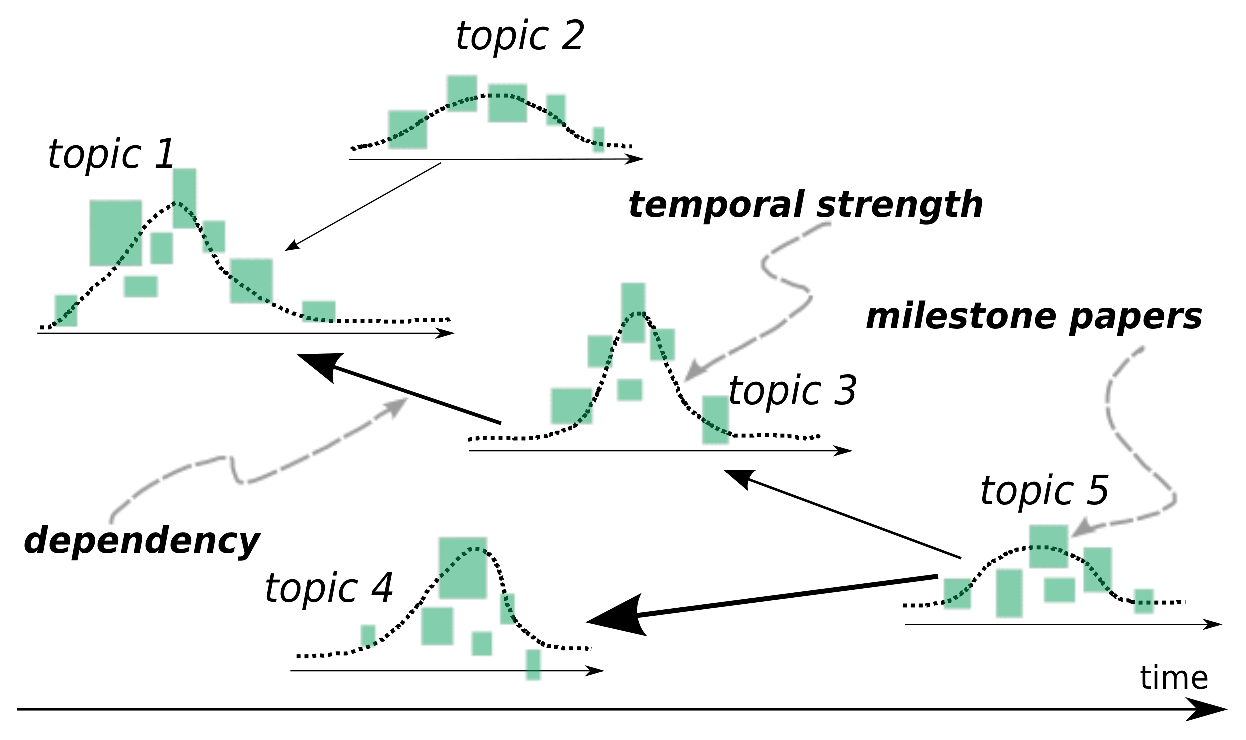
\includegraphics[scale= .6]{citation-lda/plot/fake_theme.eps}
  \end{center}
  \caption{An illustration of the proposed evolution graph. We show 5 topics,
  and their dependency. Topic 2 and 3 are enabled by Topic 1 while Topic 5 is
  enabled by Topic 3 and 4.}
  \label{fig::fake}
\end{figure}

To answer the questions raised above, ideally, we would like to automatically
construct a \emph{``research theme evolution graph''}, which we illustrate in
\Cref{fig::fake}.  With such a graph, when zooming into the scope of individual
topics, multiple types of information are provided to facilitate users to
understand the research topic:

\begin{itemize}
\item \emph{Topic Milestone Papers}: It is critical to recognize the papers that
  are best representative for a topic in the course of understanding topics. We
  refer to them as ``topic milestone papers''. Milestone papers of a topic
  provide a good picture how a topic is formed. In \Cref{fig::fake}, milestone
  papers are shown in each topic as rectangles and the ``size'' reflects their
  importance with respect to topics.
\item \emph{Topic Temporal Strength}: The relative popularity of topics at
  different times reveals the temporal nature of topics, which can help users to
  identify \emph{current} vs. \emph{previous} research topics as well as the
  rough topic life spans. Intuitively, when many milestone papers occur, the
  topic draws more attention and becomes popular.
\item \emph{Topic Keywords}: Extracting keywords that can properly summarize a
  topic would enable users to obtain a brief idea about the topic even without
  reading its relevant papers, allowing users to fast navigate among topics in
  search of the most interesting ones.
\end{itemize}

While zooming out to see the big picture of all related topics in the theme,
there is also meaningful information to explore:
\begin{itemize}
\item  \emph{Topic Importance}: Quantifying the importance of topics helps a
  user to discriminate the \emph{major} vs. \emph{minor} topics in a research
  theme. Topic importance also reflects how well the topic is recognized by the
  community.
\item \emph{Topic Dependency}: Many new topics are built on top of the old ones.
  Discovering the dependency relation between topics provides a good guidance
  for users when searching for \emph{origin/continuing} topics. In
  \Cref{fig::fake}, we visualize the dependency strength between topics by the
  ``thickness'' of edges.
\item \emph{Evolution Patterns}: Connecting topics by their dependency
  illustrates the underlying evolution patterns for research themes. Is there
  any trend that different topics get merged together to form a new
  (interdisciplinary) topic, such as Topic~3 and Topic~4 are merged into
  Topic~5? Or is there a general topic branched into multiple topics that
  address specialized problems, such as Topic~1 has led to Topic~2 and Topic~3?
\end{itemize}

To automatically construct such an evolution graph as shown in \Cref{fig::fake},
the two major computational tasks are:
\begin{itemize}
\item \textbf{\emph{Discovering the research topics}}, which includes finding
  milestone papers, computing the temporal strength, and extracting keywords for
  each individual topic.
\item \textbf{\emph{Discovering the theme evolution}}, which includes
  identifying the topic importance and learning the dependency relation between
  topics, as well as recognizing the underlying evolution patterns.
\end{itemize}

Existing approaches, notably those of topic modeling, can generate some (not
all) of these components in the evolution graph, but they are far from adequate
for the following reasons: First, though there are many works that aim to
construct evolution map over time, they rely on pre-segmentation of text streams
into fixed time windows, due to either computational
issue~\cite{blei2006dynamic,mei2005discovering,wang2006topics} or modeling
issue~\cite{wang2012continuous}. Consequently, the topic evolution result would
be inevitably sensitive to the choice of temporal granularity of how time is
discretized and sliced. Suboptimal granularity of time might result in missing
important topics or even lead to inaccurate evolution analysis.  Second, the
edges in most of the existing evolution graphs, do not reflect the
\emph{dependency relation} between topics, and can only reveal the \emph{topic
similarity} and \emph{correlation}
~\cite{blei2006dynamic,blei2007correlated,mei2005discovering,wang2012continuous}.
The fundamental limitation is that content-based topic modeling approaches are
built on \emph{word co-occurrence}, which essentially is \emph{undirected}
unlike the dependency relation.  Third, it is difficult for any aforementioned
models (including Pairwise Link-LDA~\cite{nallapati2008joint}) to assess the
impact of documents with respect to different topics, i.e., identifying the
milestone papers. Their approaches model topics as distributions over words, and
although the text similarity between document and topic can be computed, it
would be a substantially different measurement from the document \emph{impact}
on a topic.

As hinted above, a major reason why existing topic models are insufficient is
that they have not fully exploited citation relations to discover topics. In
this chapter, we address these limitations by doing joint analysis of citations
and text.  Indeed, we will rely  more on citation links than on document
content, which makes our work different from~\cite{nallapati2008joint} and all
others. Specifically, we leverage a similar idea to topic modeling and analyze
the citation graphs in a \emph{probabilistic} manner. We directly model the
generation of citations, which are direct evidence related to \emph{``impact''}
of document as well as \emph{``dependency''} between topics. Through citation
generation, we are enabled to address the core problem of assessing milestone
papers based on impact, and estimating the topic dependency.  More importantly,
our key insight here is that ``co-cited papers'' are good indicators of research
topics, more effective than relying on text similarity as in most existing work.
Empirical study~\cite{boyd2009reading} has already noticed that it is a
subjective yet difficult task to annotate for each word its belonging topic even
manually. However, for citations in a published paper written by experienced
authors, it would be much easier to determine the topic since most authors make
citations prudently and thus citation is much \emph{less noisy} than text.

To discover topics based on citations, we propose a novel probabilistic approach
to analyze citations by viewing citation graphs as a set of ``citation
documents'' where each is a research paper represented as a \emph{``bag of
citations''}. A paper that cites $k$ other (possibly duplicated) papers would
simply be viewed as a \emph{``document''} with $k$ \emph{``tokens''}, each
corresponding to the ID of a cited paper. With this view, we can model all these
citation documents with a generative topic model where we introduce latent topic
variables over the citations. This is analogous to the application of a
probabilistic topic model to model topics in text documents, but with the
important difference that the discovered topics with our model would be
characterized by a (multinomial) \emph{distribution over research papers},
rather than over words as in conventional content-based topic models. In
addition, when combined together with additional information, particularly the
\emph{published time} and the \emph{title} of each paper, our model can address
the computational tasks of discovering both \emph{the research topics} and
\emph{the theme evolution}, and constructing \emph{the evolution graph} as well.

In the rest of the chapter, we first review some of the related work in
\Cref{sec::citation-related}, which is followed by presenting our probabilistic
model for literature citations in \Cref{sec::citation-model}. After the
derivation about one specific model Citation-LDA, we focus our discussion on how
to construct the theme evolution graph in \Cref{sec::citation-graph}. Experiment
setup and extensive evaluation results will be given in
\Cref{sec::citation-exp}. Finally, we conclude our work with future direction in
\Cref{sec::citation-conclusion}.

\section{Related Work}\label{sec::citation-related}

In recent years, many literature search engines as well as digital libraries
have come into use, including Microsoft Academic
Search~\footnote{http://academic.research.microsoft.com/}, Google
Scholar~\footnote{ http://scholar.google.com/}, DBLP~\footnote{
http://www.informatik.uni-trier.de/~ley/db/} and ACM Digital
Library~\footnote{http://dl.acm.org/}. They provide knowledge about scientific
literatures through ranking and search interface, which in turn, relies on
algorithms that utilize citation-related indicators such as
H-index~\cite{hirsch2005index} and Impact Factor~\cite{garfield2006history}.

In the research community, one thread of study treats scientific literature as
citation graphs. To assess the importance of papers, graph ranking algorithms
such as PageRank and its variants have been
applied~\cite{ghosh2011time,radev2009acl,sayyadi2009futurerank,walker2007ranking}.
In~\cite{ghosh2011time}, the authors further take time into consideration in
order to overcome the recency bias that favors ``old'' papers. Apart from this,
graph clustering is investigated to identify meaningful topics, such
as~\cite{bolelli2006clustering,flake2004graph,popescul2000clustering,
qazvinian2008scientific}. In~\cite{popescul2000clustering}, it is pointed out
that efficient graph clustering can be combined with temporal information to
identify the trends of topics in literature.  Particularly, one recent
paper~\cite{jo2011web} is close to our work. It leverages both citation and
text~(title and abstract) to generate the evolution map in computer science
community. Specifically, their method relies on the temporal order of papers and
the document language model to detect the formation of new topics, and then it
computes the strength between two topics with the ``cross citation
count''~(total citation numbers between the two topics), which however ignores
the directed relation of topic dependency.  Their method is difficult to be
applied to address our problem because their method does not distinguish the
difference in topic importance, nor does it recognize milestone papers through
assessing the impact based on citations.

While on the other hand, existing probabilistic topic modeling over
text~\cite{blei2003latent,griffiths2004finding,hofmann2001unsupervised} has been
throughly studied, treating documents as mixtures of latent topics.  Early
attempt in modeling the topic evolution~\cite{mei2005discovering} investigates
the Probabilistic Latent Semantic Index~(PLSI)~\cite{hofmann2001unsupervised} to
extract topics and models the evolution process as transitions between topics in
Hidden Markov Model~(HMM).  Later, Topic Over Time~(TOT)
model~\cite{wang2006topics} is developed based on Latent Dirichlet
Allocation~(LDA)~\cite{blei2003latent}. The key difference between between LDA
and TOT is that TOT explicitly assumes time as generated from topics, which
jointly models time and word, thus enabling itself to discover time-aware topics
as well as topic temporal strength.  Besides, Dynamic Topic
Models~\cite{blei2006dynamic,wang2012continuous} address the problem of topic
evolution by modeling topics~(distributions over words) changing over time. In
the discrete case~\cite{blei2006dynamic}, topics at the next time-stamp deviate
from the current ones by a Gaussian noise; while, in the continuous
case~\cite{wang2012continuous}, the change of topics over time is generalized as
Brownian motion.  One limitation of these models~\cite{blei2006dynamic,
mei2005discovering,wang2012continuous,wang2006topics} is that they all rely on
the pre-segmentation of time: without appropriate time granularity selected,
they could fall into difficulty in finding important topics. Ideally, the
selection of correct time span should be made automatically.  In addition to
these studies, others consider the problem of modeling topic
correlation~\cite{blei2007correlated} and document hyperlink
generation~\cite{chang2009relational}, for which the essential difficulty is
that they cannot model the \emph{``dependency''} relation between topics. The
only exception we are aware of so far is the paper~\cite{nallapati2008joint}
which jointly models text and citation generatively. One of its proposed model,
named ``Pairwise Link-LDA'', explicitly includes the topic dependency as model
parameters by extending the idea of mixed-membership block stochastic
models~\cite{airoldi2006mixed}. In words, the chance of generating a particular
citation is determined by the topics of citing and cited documents, which indeed
addresses the topic dependency directly. Nevertheless, the Pairwise Link-LDA is
not able to fulfill all the tasks we listed such as recognizing the milestone
papers and so on.


To our best knowledge, there is no existing approach that can address all the
questions as we raised before, i.e., the discovery of \emph{research topics} and
\emph{theme evolution}. To this end, we directly model the generation of the
citation links among literatures in this work. In the same spirit of topic
modeling, citations are generated stochastically according to a distribution
with respect to the underlying topic. It is worth noting that applying the topic
modeling approaches to study graphs was previously investigated for discovering
communities from coauthorship networks in
\cite{henderson2009applying,zhang2007lda}. Nevertheless, our model not only
discovers the topics, but also explores their dependency relationships and
yields meaningful knowledge about the evolution of topics.

\section{Probabilistic Modeling of Literature
Citations}\label{sec::citation-model}

In contrast to most existing work on citation analysis, where citations are
often modeled as network or graph, we propose to represent citation graph as a
set of ``citation documents'' where each is a research paper represented as
``bag of citations'', and model these citation documents with a probabilistic
generative model.  Such a new approach has several advantages over pure graph
analysis methods.  First, by using a latent topic variable, we can naturally
associate topics with papers and citations, enabling ranking the paper based on
citation within each topic, through which milestone papers can be identified.
Second, by modeling the whole set of papers in a field, we can obtain a set of
topics that summarize well the major research topics in the field, with
(probabilistic) weights quantifying their importance.  Third, by estimating the
topic level citation structure, it is possible to compute the strength of
dependency relation between topics and picturing the evolution paths of research
themes.  Last, distribution over papers for each topic obtained by such a model
can be easily used to compute a distribution over time or keywords when used
together with other information such as paper published time and title, allowing
modeling the topic temporal strength and summarizing topics with keywords.

Compared with pure content-based topic models, our use of topic model is
entirely on capturing topics through citation structures, roughly corresponding
to discovering topics based on \emph{co-citation relation}, which is intuitively
more accurate in finding research topics: if there is a \emph{``stable''} set of
\emph{``core papers''} that are often cited together, then it generally
indicates the existence of a major research topic and the core papers are
actually \emph{milestone papers} in that topic. Specifically, we use a
probabilistic model to explain how an author generates the references
(citations) for a paper (which we may also refer to as a document for
convenience sometimes).  More specifically, given a paper, he/she would
``generate'' all the references cited in the paper independently.  When
generating each citation, the author would first sample a topic according to a
document-specific topic distribution~($doc\_topic$ distribution), and then draw
a reference document to cite from the citation distribution of the sampled
topic~($topic\_doc$ distribution).  One may easily notice that such a generation
process is essentially similar to the one over words for documents assumed in
probabilistic topic models for text data.  Indeed, our work is a novel way of
using topic models for citation analysis, and just as topic models are very
effective for discovering and analyzing topics in \emph{text documents}, our
model can also be very useful for discovering and analyzing topics in
\emph{scientific literatures} where the citation graph is available. Another
advantage over content-based topic models we may anticipate is that the
computational complexity is greatly reduced because the number of citations is
much less than the number of words in the corpora.

\subsection{The General Model}

Formally, suppose each document $d$ cites a subset of other documents
$\{c_t\}$~$(t=1,2,\ldots)$, where $c_t$ is a cited reference. We
assume the following generation process for a citation that links to document
$c_t$ in document $d$ (i.e., document $d$ cites document $c_t$):

\begin{itemize}
\item  Draw topic sample: $z_t \sim D_{doc\_topic}(z;d)$
\item  Draw citation sample: $c_t \sim D_{topic\_doc}(c;z_t)$
\end{itemize}

The doc-topic distribution $D_{doc\_topic}(\cdot;d)$ and topic-doc distribution
$D_{topic\_doc}(\cdot;z)$ are parameterized by the citing document $d$ and the
topic $z$ respectively, and are the two key components in the model that would
enable many interesting ways to analyze topics and evolution relations among
topics.  Indeed, $D_{doc\_topic}(\cdot;d)$ gives us a probability distribution
over (latent) topics conditioned on document $d$, and can be interpreted as the
\emph{topic coverage} in document $d$ when generating citations, whereas
$D_{topic\_doc}(\cdot;z)$ gives a \emph{``reverse''} conditional distribution of
documents given a topic, and can be interpreted as how a topic is characterized
by a set of papers (documents) that are cited.  Thus if a document $c_i$ has a
higher probability than $c_j$  according to  $D_{topic\_doc}(\cdot;z)$, it would
suggests that $c_i$ better characterizes topic $z$ than $c_j$, or $c_i$
represents topic $z$ better as being a more important paper with higher impact
upon $z$ than $c_j$.  With such a distribution over papers, we can easily
compute the \emph{expected time} for a topic based on the time when the paper
was published as well as the \emph{topic keywords} based on the paper titles (or
abstracts if available).  Note that a substantial advantage of such a
probabilistic model is that it can \emph{``decode''} why document $d$ cites
document $c_t$ by inferring the latent topic associated with this citation
relation and quantifying with uncertainty, which enables ``disambiguation'' of
citation relations to some extent.  As will be further discussed, we can use
such a model to perform the computational analysis for discovering research
topics and theme evolution, which finally lead to the construction of evolution
graph as proposed in \Cref{fig::fake}.


\subsection{Citation-LDA}

Though we may have different ways to refine the general probabilistic model
defined above, in this work as a first step, we focus on exploring the use of
the basic Latent Dirichlet Allocation (LDA)~\cite{blei2003latent} model, which
we call ``Citation-LDA'' and show that even with this simple model setting, we
can already discover a lot of interesting knowledge that is useful for
understanding research theme evolution.

Specifically, Citation-LDA assumes that $D_{doc\_topic}$ and $D_{topic\_doc}$
are multinomial distributions with parameters drawn from conjugated Dirichlet
prior $\alpha$ and $\beta$ respectively~\footnote{In experiments, $\alpha$ and
$\beta$ are symmetric prior with weight $\num{1e-3}$ to encourage sparse topic
distributions}. We follow the convention to denote $D_{doc\_topic}(\cdot;d)$ and
$D_{topic\_doc}(\cdot;z)$  by $\theta_d$ and $\phi_z$ respectively, and we have:
$\theta_d \sim \mathrm{Dir}(\alpha)$ and $\varphi_z \sim \mathrm{Dir}(\beta)$.
The citation generation process for document $d_{i^*}$ is:

\begin{itemize}
\item Sample a topic $z=k^* \sim \mathrm{Multi}(\theta_{i^*})$
\item Sample a document to cite $c = d_{j^*} \sim \mathrm{Multi}(\varphi_z)$
\end{itemize}

We use the collapsed Gibbs sampling~\cite{griffiths2004finding} to make
inferences with the model.  The sampling is initialized by assigning random
topic labels $\{z\}$ and updates each of them iteratively. In particular, for
the $t$-th citation that links to $d_{j^*}$ in document $d_{i^*}$, the topic
assignment is updated according to the probability~\footnote{We use $\#(\cdot)$
  as the \emph{count} function that computes the number of instances satisfy the
  conditions specified in $(~)$, and $\neg (i^*, t)$ denotes all the citations
except the $t$-th citation in document $d_{i^*}$}:

\begin{align}
  & \Pr( z = k^* |  c_{i^*, t} = d_{j^*},  Z_{\neg (i^*,t)}, C^{\neg (i^*, t)} )
  \nonumber \\
  \propto &
  \left(\alpha_{k^*} + \#^{\neg (i^*, t)} (z = k^*, d=i^*) \right)
  \times
  \frac{\beta_{j^*} + \#^{\neg (i^*, t)} (z= k^*, c = d_{j^*} )}{
      \sum\limits_j \beta_{j} + \#^{\neg (i^*, t)} (z= k^*, c = d_{j} )}
  \label{eq::citation_eq_samp}
\end{align}

The sampling converges to the true posterior distribution after the burn-in
stage~\footnote{In experiments, this is empirically measured by
parallel gibbs sampling}. Posterior expectation of $\theta_{i^*,k^*}$ and
$\varphi_{k^*, j^*}$ is given by~\footnote{We use $\langle \cdot
\rangle$ to denote averaging the statistics specified over the iterations in
sampling}:

\begin{align}
\hat\theta_{i^*,k^*}  =
  \left\langle \frac{\#(d= i^*, z = k^*) + \alpha_{k^*}}{
                \sum\limits_k \#(d= i^*, z = k) + \alpha_{k}}
  \right\rangle\label{eq::citation_eq_theta}\\
\hat\varphi_{k^*, j^*} =
  \left\langle \frac{\#(z = k^*, c = j^*) + \beta_{j^*}}{
                \sum\limits_j \#(z = k^*, c = j) + \beta_{j}}
  \right\rangle\label{eq::citation_eq_phi}
\end{align}

In addition, the empirical posterior  distribution over topics can be computed
as:

\begin{equation}
  \hat\Pr(z=k^* | C) =
  \left\langle \frac{\#(z = k^*)}{\sum\limits_k \#(z=k) } \right\rangle
  \label{eq::citation_eq_topwei}
\end{equation}

\section{Construction of Theme Evolution Graph}\label{sec::citation-graph}

The results obtained from
\Cref{eq::citation_eq_theta,eq::citation_eq_phi,eq::citation_eq_topwei} form the
basis for exploring the knowledge that leads to the construction of the
evolution graph, which includes the discovery of not only individual research
topics but also theme evolution.  We investigate them in details in following
discussion.

\subsection{Discovery of Research Topics}

Zooming into individual topics identified by Citation-LDA, we are interested in
finding \emph{milestone papers}, generating \emph{keywords}, and computing the
\emph{temporal strength} for each topic.

\subsubsection{Topic Milestone Papers}

The \emph{topic-doc} distribution $\{\hat\varphi_{k,j}\}$, as computed in
\Cref{eq::citation_eq_phi} indicates how well a single paper $d_j$ represents
the topic $z_k$. The ranking of papers based on $\{\hat\varphi_{k,j}\}$ in
essence provides the topic-aware impact assessment for papers with the milestone
papers for topic $z_k$ ranked at the top.

There are advantages over naive ranking of papers based on the citation counts,
which can be inaccurate since there are cases that in one area people tend to
include more references than people from another area.  Even sophisticated
citation-based measurement,
e.g.,~\cite{ghosh2011time,radev2009acl,sayyadi2009futurerank,walker2007ranking},
without taking into account of topics, can lead to bad judgement: a well
recognized theoretic paper about graphic model in ``Bayes learning'' might
receive less credit in ``data engineering'' and ``very large database'' due to
the computational difficulty that limits its application.

\subsubsection{Topic Temporal Strength}

For topic $z_k$, there is a time point when it began attracting attention, a
time point when it enjoyed its glory days with most important milestone papers
emerged, and possibly a time point when interest decreased and the topic faded
out. If it is a long lasting topic, it might span over decades while if not, the
active period can be as short as only a few years.

Topic temporal distribution sufficiently maintains the information. Viewing
topic $z_k$ as a distribution over papers, the proportion of accumulated
probability for published papers until time $t$ forms the cumulative
distribution function~(CDF):

\begin{align}
\Pr(time \leq t |z = k)
  &= \sum\limits_{j, time(d_j) \leq t} \Pr(c=j | z=k) \nonumber\\
	&= \sum\limits_{j,time(d_j) \leq t} \hat\varphi_{k,j}
  \label{eq::citation_time1}
\end{align}

For the discrete time case, which is also our case, the probability mass
function (PMF) for temporal distribution of $z_k$ is:

\begin{equation}
  \Pr(time = t |z = k)	= \sum\limits_{j,time(d_j) = t} \hat\varphi_{k,j}
  \label{eq::citation_time2}
\end{equation}

In addition, the expectation can be computed as:

\begin{equation}
  \mathbf{E}_{c | z=k} [\mathrm{time}(c)]  =
  \sum\limits_j \mathrm{time}(d_j) \hat\varphi_{k,j} \label{eq::citation_time3}
\end{equation}

The standard deviation can also be easily computed, which, together with
\emph{topic expected time}, concisely show the major occurring time and provide
a rough estimation about the life span for a topic.

\subsubsection{Topic Keywords}

In general it would be desirable to summarize the topic with only a few
words~\cite{boyd2009reading}. With Citation-LDA, we accomplish this by
leveraging words in title (or abstract if available) as tags for each paper and
summarize the topic by those words with high \emph{expected occurrences}.
Specifically, to compute the word occurrence expectation over
$\{\hat\varphi_{k,j}\}$ for word $w$ in topic $z_k$:

\begin{equation}
  \mathbf{E}_{c | z=k} [\#(w, c)] =
    \sum\limits_j \hat\varphi_{k,j} \cdot \#(w, d_j)
\end{equation}

As shown later in experiments, the topic keywords generated from titles are
surprisingly indicative yet discriminative for especially seemingly similar
topics.

\subsection{Discovery of Theme Evolution}

In order to help a researcher see the big picture of all research topics, we can
also easily use Citation-LDA to discover the theme evolution, which would
involve the exploration of assessing the \emph{topic importance} as well as the
\emph{topic dependency relation}, and recognizing the underlying \emph{evolution
patterns}.

\subsubsection{Topic Importance}

By \Cref{eq::citation_eq_topwei}, the distribution of $\{\hat\Pr(z=k)\}$
represents the chance of documents from one topic getting cited. Consequently,
it can be associated as the topic importance in the research community since
topics with higher importance are those who receive more citations and vice
versa.  The top important topics reflect the major research progress and reveal
the dominant research interest in one area.

\subsubsection{Topic Dependency}

In Citation-LDA, topics are represented as multinomial distributions over papers
$\{\hat\varphi_{k,j}\}$ while the \emph{doc-topic} distribution
$\{\hat\theta_{i,k}\}$ implies the topic mixture of document $d_i$.  More
precisely, $\hat\theta_{i,k^{(2)}}$ is the probability of topic $k^{(2)}$
occurring in document $d_i$ with an (outlink) citation.  Consequently, when
marginalizing over papers $d_j$ discounted by $\{\hat\varphi_{k^{(1)},j}\}$, the
probability of citing topic $k^{(2)}$ (by topic $k^{(1)}$) conditioned on topic
$k^{(1)}$ is:

\begin{align}
 & \Pr(k^{(1)} \rightarrow k^{(2)} | k^{(1)}) \nonumber \\
=& \mathbf{E}_{c | z=k^{(1)}}[\Pr(z= k^{(2)} |d = c)] \nonumber \\
=& \sum\limits_j \Pr( c = j| z = k^{(1)} ) \Pr(z = k^{(2)} |  d = j) \nonumber \\
=& \sum\limits_j \hat\varphi_{k^{(1)},j} \hat\theta_{j, k^{(2)}}
  \label{eq::citation_lda_citation_structure}
\end{align}

An intuitive explanation of \Cref{eq::citation_lda_citation_structure} is:
whenever randomly drawing a document $d_j$ from topic $k^{(1)}$, and then
emitting a citation from that document, $\Pr(k^{(1)} \rightarrow k^{(2)} |
k^{(1)})$ is the chance of that citation being associated with \emph{latent}
topic $k^{(2)}$.


More importantly, \Cref{eq::citation_lda_citation_structure} explains the
\emph{topic level citation structure}, as well as quantifies the \emph{topic
dependency} between any two topics precisely --- the amount of influence of
topic~$k^{(2)}$ upon topic~$k^{(1)}$, from which we can tell if a topic is
developed on top of another.

\subsubsection{Evolution Patterns}

Topic level citation structure~{$\{\Pr(k^{(1)} \rightarrow k^{(2)} |
k^{(1)})\}_{K\times K}$} reveals the topic dependency. Nevertheless, it is
indeed a $K \times K$ matrix with most entries being sparse. In our work, we
propose two pruning criteria:

\begin{itemize}
\item \emph{Threshold cutting-off}: By setting a threshold
  $\xi$~\footnote{{$\xi = 0.1$ in experiments}} empirically, all
  citation dependencies between topics with strength less than $\xi$ would be
  removed.
\item \emph{Temporal regularization}: As previously investigated
  in~\cite{jo2011web,mei2005discovering}, the citation dependencies of the
  ``old'' topics upon the ``new'' topics can be roughly regarded as noise and
  safely discarded.
\end{itemize}

After applying pruning to the \emph{topic level citation structure}, significant
yet meaningful influences between topics are kept. Closely dependent topics form
the themes, in which different \emph{evolution patterns} can be found: some
topics may get merged into a new topic which is highly dependent on
them~(\emph{merging}). Alternatively, one topic might have multiple subsequent
topics that are developed on top of it~(\emph{branching}). In other cases,
topics stop evolution and gradually \emph{fade out}. We will discuss evolution
patterns with concrete examples in the following experiment section.



\section{Experiments \& Results} \label{sec::citation-exp}

\begin{table*}[t!]
\caption{Top 10 High Impact Papers in Topic ``Sentiment Analysis'' (Topic 89,
        AAN)}\label{tab:high_impact_aan}
\begin{tabular}{|c|c|l|}
\hline
$\hat\varphi$	& Venue &	Paper Title \\
\hline\hline
0.078533		& EMNLP'02	& 	Thumbs Up? \textbf{Sentiment Classification} Using
  Machine Learning Techniques \\
0.067202		& ACL'02		& 	Thumbs Up Or Thumbs Down? \textbf{Semantic
  Orientation} Applied To \\
  && \, Unsupervised Classification Of Reviews \\
0.048269		& HLT'05		&	  Recognizing Contextual Polarity In Phrase-Level
  \textbf{Sentiment Analysis} \\
0.043634		& ACL'04		&	A Sentimental Education: \textbf{Sentiment Analysis}
  Using Subjectivity \\
  && \, Summarization  Based On Minimum Cuts \\
0.036498		& ACL'97		&	Predicting The \textbf{Semantic Orientation} Of
  Adjectives \\
0.031173		& COLING'04	&	Determining The \textbf{Sentiment Of Opinions}	\\
0.030686		& HLT'05		&	Extracting Product Features And \textbf{Opinions} From
  \\ && \, Reviews \\
0.028673		& EMNLP'03	&	Towards Answering \textbf{Opinion} Questions:
  Separating Facts From \\
  && \, \textbf{Opinions} And Identifying The \textbf{Polarity Of Opinion
    Sentences}	\\
0.027851		& EMNLP'03	&	Learning Extraction Patterns For \textbf{Subjective
  Expressions} \\
0.016856		& ACL'05		&	Seeing Stars: Exploiting Class Relationships For
  \textbf{Sentiment Categorization} \\
  && \, With Respect To Rating Scales \\
\hline
\hline %timesorted topic
\end{tabular}

\caption{Top 10 High Impact Papers in Topic ``Air Pollution'' (Topic 175,
    PMC)}\label{tab:high_impact_pmc}

\begin{tabular}{|c|c|l|}
\hline
$\hat\varphi$	&	Venue	&	Paper Title \\
\hline\hline
0.035435 & Environ\_Health\_Perspect & Ultrafine Particulate \textbf{Pollutants}
Induce Oxidative Stress and  \\
&& \, Mitochondrial Damage \\
0.018051 & Environ\_Health\_Perspect & Ambient \textbf{Air Pollution} and
Atherosclerosis in Los Angeles \\
0.017836 & Environ\_Health\_Perspect & Effects of \textbf{Air Pollution} on
Heart Rate Variability: the \\
&& \, VA Normative Aging Study \\
0.014414 & Environ\_Health\_Perspect & Acute Blood Pressure Responses in Healthy
Adults during Controlled \\
&& \, \textbf{Air Pollution} Exposures \\
0.014233 & Environ\_Health\_Perspect	& The Effect of Particulate \textbf{Air
Pollution} on Emergency \\
&& \, Admissions for Myocardial Infarction\\
0.013984 & Environ\_Health\_Perspect & Diabetes, Obesity, and Hypertension May
Enhance Associations \\
&& \, Between \textbf{Air Pollution} and Markers of Systemic Inflammation \\
0.013690 & Environ\_Health\_Perspect & Nanotoxicology: an Emerging Discipline
Evolving from Studies \\
&& \, of \textbf{Ultrafine Particles} \\
0.013266 & Environ\_Health\_Perspect & Association of Fine \textbf{Particulate}
Matter From Different \\
&& \, Sources With Daily Mortality in Six U.S. Cities \\
0.013090 & Environ\_Health\_Perspect & \textbf{Ultrafine Particles} Cross
Cellular Membranes by  \\
&& \, Nonphagocytic Mechanisms in Lungs and in Cultured Cells \\
0.012830 & Environ\_Health\_Perspect	& \textbf{Ambient Particulate Air
Pollution}, Heart Rate Variability, \\
&& \, and Blood Markers of Inflammation in a Panel of Elderly
  Subjects \\
\hline
\hline %timesorted topic
\end{tabular}
\end{table*}

In this section, we first formally describe the two datasets AAN and PMC on
which we demonstrate our Citation-LDA. Further, extensive evaluation results of
discovery of research topics and theme evolutions are discussed. Last, we show
that our Citation-LDA over-performs conventional Content-LDA baseline with two
evaluation metrics: \emph{forward-citation} and \emph{journal conditioned
entropy}.

Due to space limit, here we only show some representative results in our work.
The complete results as well as the source code for Citation-LDA can be found
at: \url{http://sifaka.cs.uiuc.edu/~xwang95/citation_lda/}

\subsection{Dataset}

In our experiments, two public scientific literature datasets are investigated:
AAN from natural language processing domain and PMC from biomedical and life
sciences.

\subsubsection{ACL Anthology Network~(AAN)}

The ACL Anthology Network~(AAN)~\cite{radev2009acl} is a public dataset which
includes all papers published by Association for Computational Linguistics~(ACL)
and related organizations over the period from 1965 till now. Major conference
and journal papers in the area of natural language processing~(NLP) can be found
in the dataset. In our experiments, there are are in total $18,041$
papers~(including citing and cited papers) from $13$ venues with $82,944$
citations.

\subsubsection{PubMed Central~(PMC)}

The PubMed Central~(PMC)~\footnote{\url{http://www.ncbi.nlm.nih.gov/pmc/}} is a
free archive of biomedical and life sciences journal literature. Compared with
AAN, it is a much larger yet sparser dataset, with a coverage of much wider
areas than NLP. In our experiments, we includes the papers published after year
1960 and there are $145,317$ article papers with $274,133$ citations from
$1,726$ journals.

Unlike AAN, the large number of journals in PMC provide a \emph{``coarse topical
annotation''} for papers, as in life sciences journals are commonly specialized
in only a few research topics. For example, the journal \emph{``Nucleic Acids
Research''} covers research on nucleic acids such as DNA and RNA, but the
journal \emph{``Environmental Health Perspectives''} mainly publishes research
on environmental health such as toxicology, exposure science and public health,
etc. Later, we would utilize the journal information to evaluate the modeling
performance of Citation-LDA and Content-LDA.

\subsection{Results of Research Topics Discovery}

Before the discussion of the results, however, a nontrivial question is how to
determine the \emph{number of topics} to be modeled? In following experiments,
we perform the Citation-LDA with 100 topics in AAN and 500 topics in PMC,
leaving the discussion of selecting the topic number in
\Cref{sec::citation_sec_model_selection}.

\subsubsection{Finding Milestone Papers}

Milestone papers for two topics: ``sentiment analysis'' from AAN and ``air
pollution'' from PMC, both of which are of great importance, are presented in
\Cref{tab:high_impact_aan,tab:high_impact_pmc} respectively~(10 milestone papers
for each topic). Together, the \emph{topic-doc} probability $\hat\varphi_{k,j}$
and the venue/journal sources are included. Clearly, the milestone papers listed
are truly representative and recognized by the community based on the impact
with respect to the topic.

One might notice that the top milestone papers in \Cref{tab:high_impact_pmc},
unlike those of topic ``sentiment analysis'' from AAN, are actually all from one
journal ``Environmental Health Perspectives'', which is generally regarded as
among the most top tier journals in the area of ``environment health'' with
especially established reputation in the topic ``air pollution''. In fact, the
top milestone papers for topics in PMC being from the same~(or only a few)
journal(s) are actually quite common.  Given that the journals in PMC are
closely related to a variety of specialized topics, it can be taken as ``noisy''
topic labels of fair quality for evaluation purpose.

\begin{figure}[h!]
  \begin{center}
    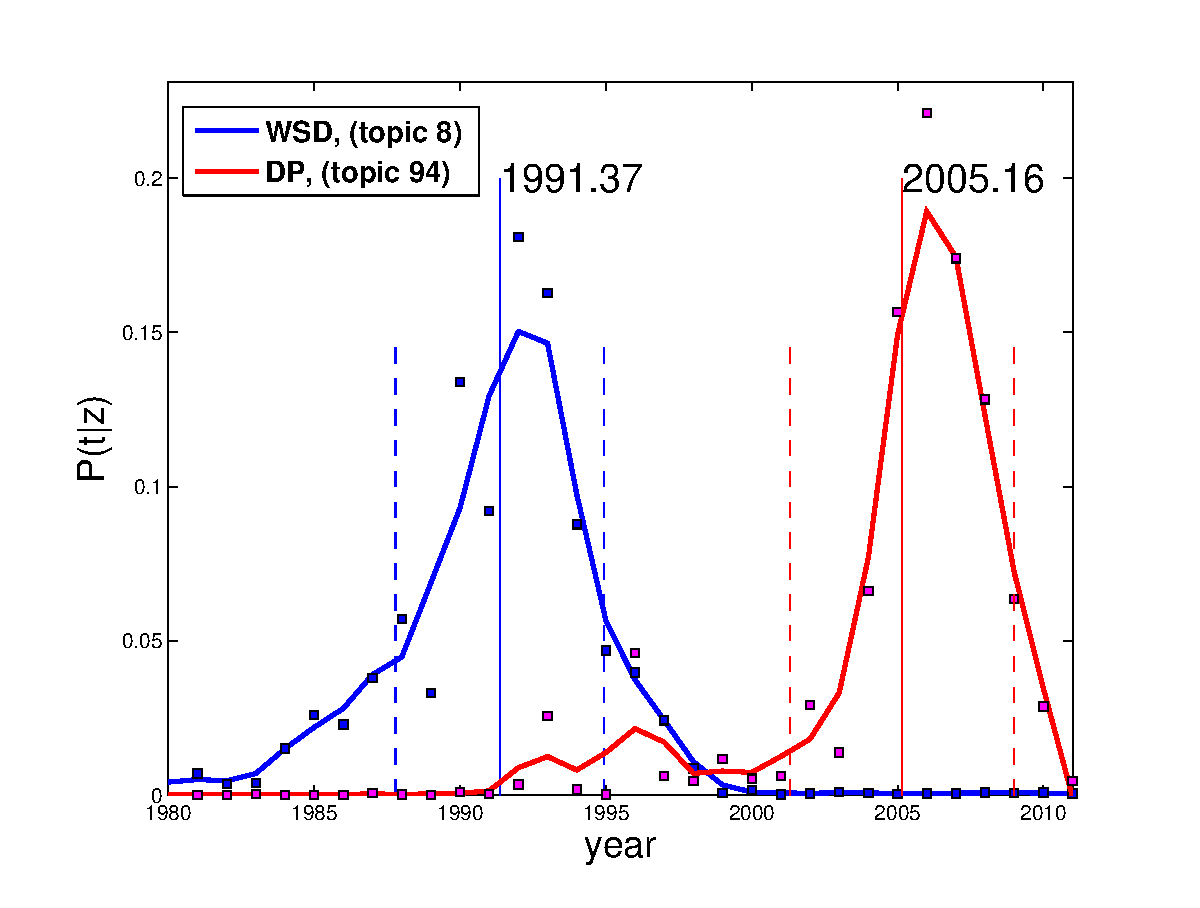
\includegraphics[scale= .5]{citation-lda/plot/aan_wsd_pd.eps}
  \end{center}
  \caption{Topic Temporal Strength for ``WSD'' and ``DP''}
  \label{fig::citation_aan_wsd_pd}
\end{figure}

\subsubsection{Discovering Temporal Strength}

To demonstrate that our model discovers the topic over time correctly, we show
the topic temporal strength of two topics, namely ``word sense
disambiguation''~(WSD) and ``dependency parsing''~(DP) from AAN in
\Cref{fig::citation_aan_wsd_pd}, and the computational details can be found in
\Cref{eq::citation_time1,eq::citation_time2,eq::citation_time3}.

In fact, the topic ``WSD'' was once a popular topic around early 90s while
``DP'' was newly popularized around year 2005. Based on our model, ``WSD'' has
the expected time $1991.37$, with a standard deviation $3.58$. For ``DP'', the
expectation is $2005.16$ and standard deviation is $3.84$. These estimations are
all consistent with the expert knowledge.

\subsubsection{Extracting Topic Keywords}

We list the extracted keywords~(phrases)~\footnote{Top word phrases are
generated from top 20 keywords and then matched with n-grams in titles of the
milestone papers} in \Cref{tab:aan,tab:pmc}. As will be explained in details
later, the topics are the dominant 10 topics in AAN and PMC datasets.  The
extracted keywords are mainly about the \emph{problem, task, model} and
\emph{methodology} of the topics.  For Topic~73 in AAN, it shows that the topic
investigates the problem of ``part-of-speech tagging'', models the problem as
``sequential labeling'', and approaches it with  ``discriminative parsing''
methods.  For Topic~61 in PMC, the nature of the topic can be recovered as
research on the risks of ``children exposure'' against ``agricultural spraying''
such as ``pesticides'' and ``organophosphorus''. In general, it is easy to
conclude the research problems or detailed methodology for each topic through
the extracted keywords along.  Besides, based on the spotted keywords, Topic~92,
Topic~96, Topic~80, and Topic~50 in AAN are all about the research theme
``statistical machine translation''.  But keywords reveal that topics differ
from each other as concerning about \emph{distinct} methods/models~(phrase-based
models~{\scriptsize (92)} \emph{v.s.} discriminative learning~{\scriptsize
(96)}) or problems~(reordering, alignment~{\scriptsize (80)} \emph{v.s.}
evaluation~{\scriptsize (50)}), which evidently substantiates that the keywords
are adequately discriminative even for quite related topics, serving as accurate
yet succinct summary for topics.

\begin{table*}
\caption{Dominant 10 Topics in AAN (100 topics)}\label{tab:aan}
\begin{center}
\begin{tabular}{|c|c|c|c|l|}
\hline %timesorted topic
Topic 	& Weight	 	&$\mathbf{E}(t)$ & $\mathrm{stdev}(t)$ &
  Top Keyword Phrases\\ \hline \hline
94		& 0.02806	& 2005.16		& 3.84	&
  dependency parsing, non-projective, shared tasks, multilingual\\
89		& 0.02761	& 2004.64		& 3.25	&
  sentiment classification, opinion analysis, orientation, learning \\
8		  & 0.02509	& 1991.37	  & 3.58	&
  word sense disambiguation, lexical semantics \\
92		& 0.02428	& 2004.98		& 3.26	&
  machine translation, phrase-based models, alignment \\
96		& 0.02277	& 2005.45		& 3.59	&
  machine translation, online, margin, discriminative learning \\
84		& 0.02093 & 2003.94		& 3.36	&
  semantic role labeling, shared tasks \\
80		& 0.02069	& 2003.44		& 3.83	&
  machine translation, reordering, alignment \\
73		& 0.01965	& 2002.76		& 4.09	&
  discriminative parsing, sequential labeling, part-of-speech \\
50		& 0.01908	& 2000.87		& 4.13	&
  machine translation, minimum error rate training, BLEU evaluation \\
72		& 0.01804	& 2002.74		& 4.45	&
  coreference resolution, machine learning, anaphora, pronoun \\ \hline\hline
\end{tabular}

\caption{Dominant 10 Topics in PMC (500 topics)}\label{tab:pmc}
\begin{tabular}{|c|c|c|c|l|}
\hline
Topic 	& Weight	&$\mathbf{E}(t)$ & $\mathrm{stdev}(t)$ &
  Top Keyword Phrases\\ \hline \hline
484		& 0.00624	& 2006.45	&8.95		&
  protein, molecular interaction, biomolecular, database\\
499		& 0.00504	& 2007.36	&9.89		&
  ensemble, gene, genome, resources \\
488		& 0.00478	& 2006.48	&19.37	&
  gnome-scale metabolic reconstruction, escherichia coli, malaria\\
175		& 0.00450	& 2004.48	&10.67	&
  air pollution, ambient particulates, heart rates, exposure\\
373		& 0.00388	& 2005.35	&11.77	&
  non-coding RNA, sequence alignment, structure prediction, genome \\
492		& 0.00382	& 2006.56	&11.39	&
  sorcerer II, global ocean sampling, metagenomics, atlantic \\
61		& 0.00351	& 2003.22	&12.12	&
  children exposure, agricultural spraying, pesticides, organophosphorus \\
2		& 0.00350	& 1998.00	&13.85		&
  yeast, actin,saccharomyces cerevisiae, protein, myosin, cell \\
38		& 0.00338	& 2002.67	&12.78		&
  cell,	regulatory T cell, CD4, CD25, human, Foxp3, expression, induction \\
86		& 0.00320	& 2003.64	&14.12		&
  phthalate exposure, human, urine, infants, metabolites, prenatal, health \\
  \hline\hline
\end{tabular}
\end{center}
\end{table*}

\subsection{Results of Theme Evolution Discovery}

\subsubsection{Identifying Important Topics}

As earlier implied, \Cref{tab:aan,tab:pmc} show the dominant 10 topics for AAN
and PMC, which are selected based on the topic weight $\{\hat\Pr(z=k)\}$ as
computed in \Cref{eq::citation_eq_topwei}. Identified dominant topics cover
major research progress and interest in NLP and life sciences. In AAN,  it is
obvious that the research theme ``statistical machine translation'' plays the
most important role in the community, thriving and diverse with multiple
different topics such as Topic~92, 96, 80, and 50. In PMC, many topics related
to ``public health'' are dominant such as Topic~175, 61, and 86, though the
detailed research topics are distinguishable from the keywords.

\begin{figure}[h!]
  \centering
  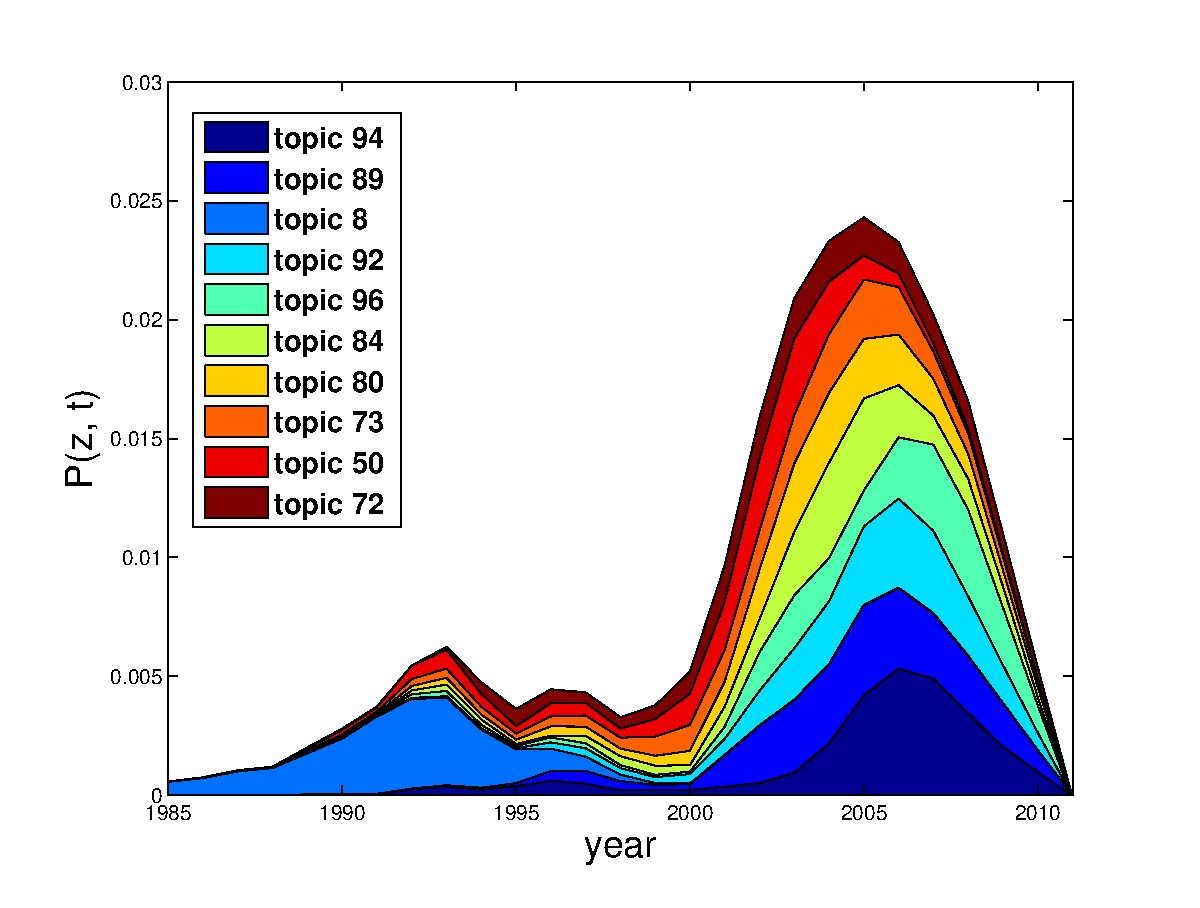
\includegraphics[scale=0.60
    ]{citation-lda/plot/AAN_10_temporal_stack_joint_smooth.eps}
  \caption{Topic-Temporal Joint Strength In AAN}\label{fig:tt_aan}
  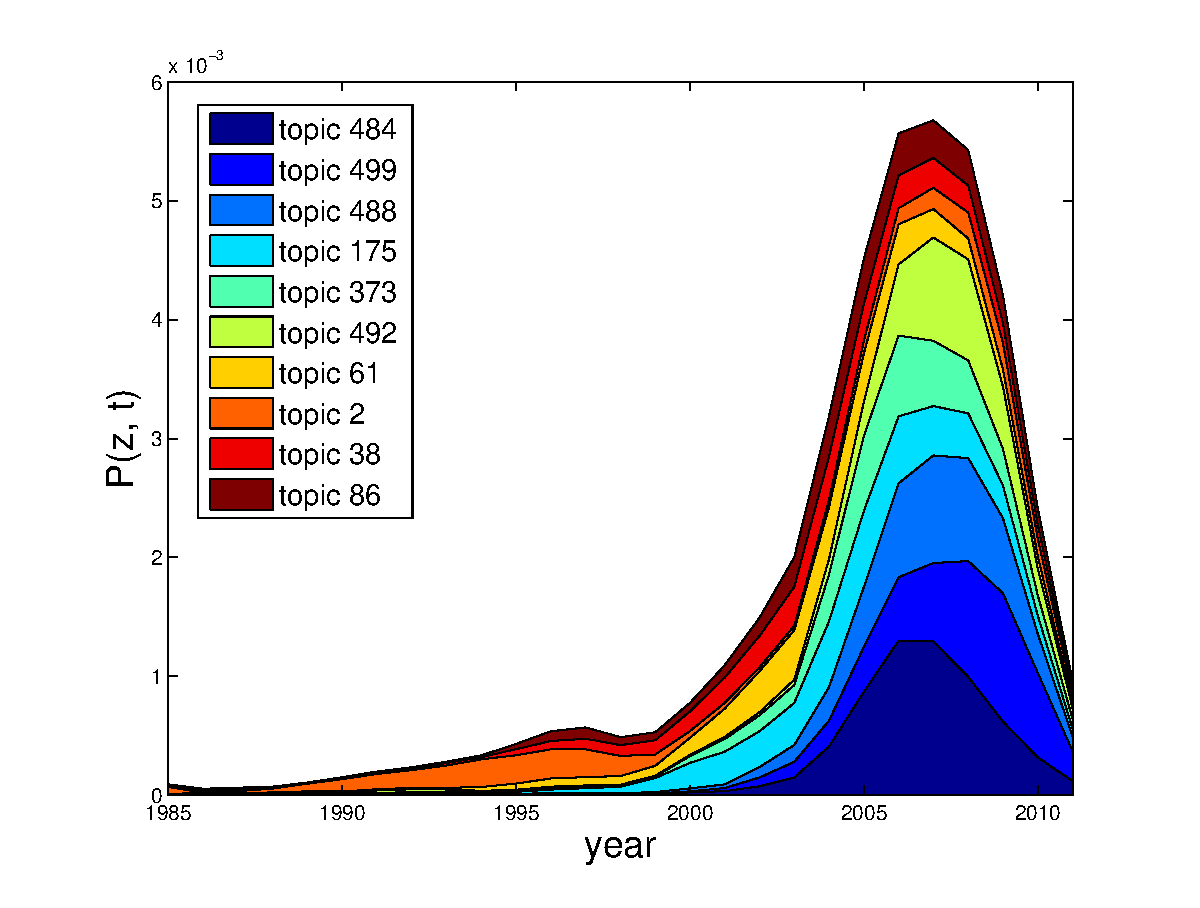
\includegraphics[scale=0.60
    ]{citation-lda/plot/PMC_10_temporal_stack_joint_smooth.eps}
  \caption{Topic-Temporal Joint Strength In PMC}\label{fig:tt_pmc}
\end{figure}

Taking the topic temporal strength into account,  $$\Pr(z=k,time=t) = \Pr(time =
k | z = k) \cdot \hat\Pr(z = k)$$ is the joint probability of topic strength and
time, allowing us to compare the topic strength in different time periods
\emph{with each other topics}. We visualize this for AAN and PMC in
\Cref{fig:tt_aan,fig:tt_pmc}, and it shows that the major research development
occurred after year 2000 for both two dataset~\footnote{However, there is
  possibility that our datasets are biased as being rich in citations after year
2000}, except that Topic 8 (``word sense disambiguation'') of AAN was dominant
compared with others in early 90s while Topic 2 of ``yeast'', ``saccharomyces
cerevisiae'' in PMC was a extensively studied around entire 90s.

\subsubsection{Topic Dependency \& Evolution Patterns}

\begin{figure}[h!]
  \begin{center}
  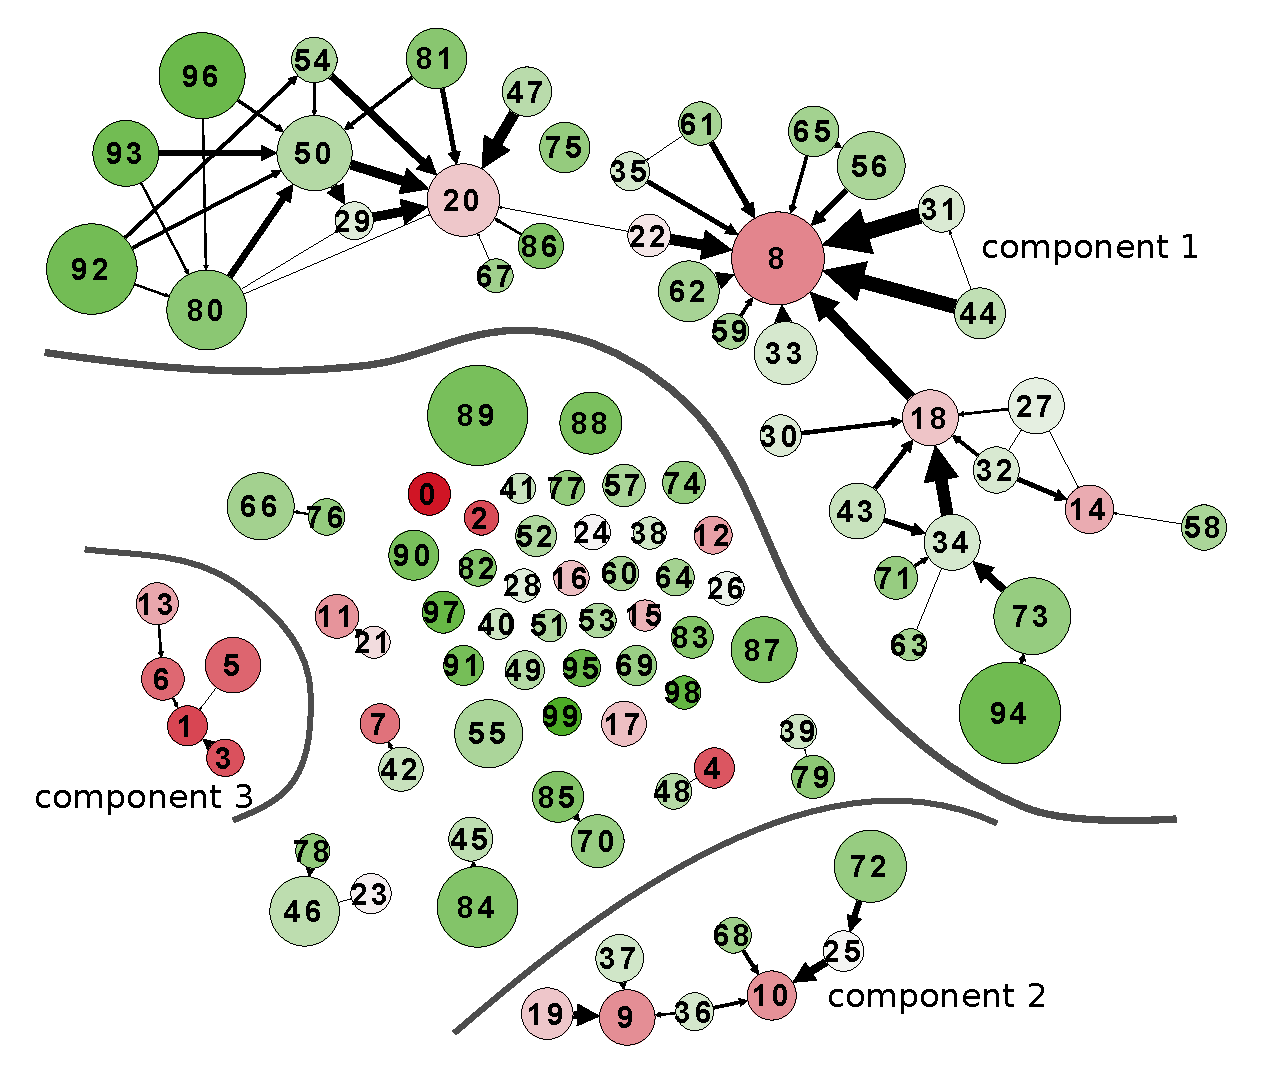
\includegraphics[scale=.7]{citation-lda/plot/full_color_with_labels}
  \caption{Theme Evolution Graph of AAN}
  \label{fig:full}
  \end{center}
\end{figure}

After applying the pruning to the \emph{topic level citation structure} the
evolution graph for research themes can be plotted.  We show the evolution graph
of AAN with 100 topics in \Cref{fig:full}: each node represents a topic
and the importance of topics are discriminated by the size of nodes. The green
nodes are new topics while the red ones are \emph{relatively} old. In addition,
the dependency between topics are reflected by the thickness of edges .

There are three major connected component, each of which contains themes
developing over time: Component 3 is about the theme ``grammar'', and
corresponding topics entirely \emph{faded out} during early 90s. Nevertheless,
Component 2 has the theme of ``discourse/dialogue'' and ``summarization'',
showing mildly progress recently (e.g., Topic 72~(2003) of \emph{``machine
learning'' based ``coreference resolution''}).  Observing the Component 1, which
is the largest, is interesting with discovery of various theme evolution
patterns: Topic 8~(1991) about ``word sense disambiguation'' was \emph{branched}
into many topics, with one of them (Topic 18) being about ``prepositional phrase
attachment''~(1994).  Soon, Topic 18 further enabled Topic 34~(1999) of
``statistical parsing'', and again Topic 73 of ``discriminative parsing'' was
established by 2003 on top of Topic 34. Later, Topic 94 of ``dependency
parsing'' raised and has grown as one dominant topic since 2005.

\begin{table*}[t!]
\caption{SMT Example for Theme Evolution}
\label{tab:smt_ex}
\begin{center}
\begin{tabular}{|c|c|c|l|l|}
\hline
Topic &Year & Paper ID & Paper Title & $\hat\varphi$ \\ \hline \hline
\multirow{4}{*}{Topic 20}
%Cluster 17 Time 20
          & 1990 & P1 &
  A Statistical Approach To Machine Translation & $0.036542$ \\
					& 1991 & P2 &
  A Program For Aligning Sentences In Bilingual Corpora & $0.047619$ \\
					& 1993 & P3 &
  The Mathematics Of Statistical Machine Translation: &\\
  &&& \; Parameter Estimation & $0.060931$\\
  \hline
%Cluster 28 Time 29
\multirow{3}{*}{Topic 29} 	& 1996 & P4 &
  HMM-Based Word Alignment In Statistical Translation & $0.097162$\\
					& 1997 & P5 &
  Decoding Algorithm In Statistical Machine Translation & $0.030390$\\
					& 1999 & P6 &
  Improved alignment models for statistical machine translation & $0.036367$\\
  \hline
%Cluster 56 Time 50
\multirow{7}{*}{Topic 50}
          & 2002 & P7 &
  BLEU: A Method For Automatic Evaluation Of Machine &\\
  &&& \; Translation & $0.087902$ \\
          & 2002 	& P8 	&
  Discriminative Training \& Maximum Entropy Models For &\\
  &&& \; Statistical Machine Translation & $0.027799$\\
					& 2003 & P9 &
  Minimum Error Rate Training In Statistical Machine & \\
  &&& \; Translation & $0.027027$\\
  \hline
%Cluster 39 Time 93
\multirow{4}{*}{Topic 93}
          & 2003 & P10&
  Statistical Phrase-Based Translation & $0.036239$\\
					& 2005 & P11&
  A Hierarchical Phrase-Based Model For Statistical Machine &\\
  &&& \; Translation & $0.022442$ \\
					& 2007 & P12&
  Hierarchical Phrase-Based Translation & $0.043163$\\
  \hline\hline
\end{tabular}
\end{center}
\end{table*}

Another key thread of theme in Component 1 was initiated by Topic 20, which was
the very beginning topic of the theme ``statistical machine translation''~(SMT).
The topics along the theme evolution path are presented in \Cref{tab:smt_ex},
including 4 topics~(Topic 20, 29, 50, and 93), together with the milestone
papers~(top 3 for each). In addition, the temporal distribution over time is
given in \Cref{fig:smt_temporal}, where the citations among the milestone
papers, and the dependency strength between consecutive topics are also
depicted.


\begin{figure}[h!]
  \begin{center}
    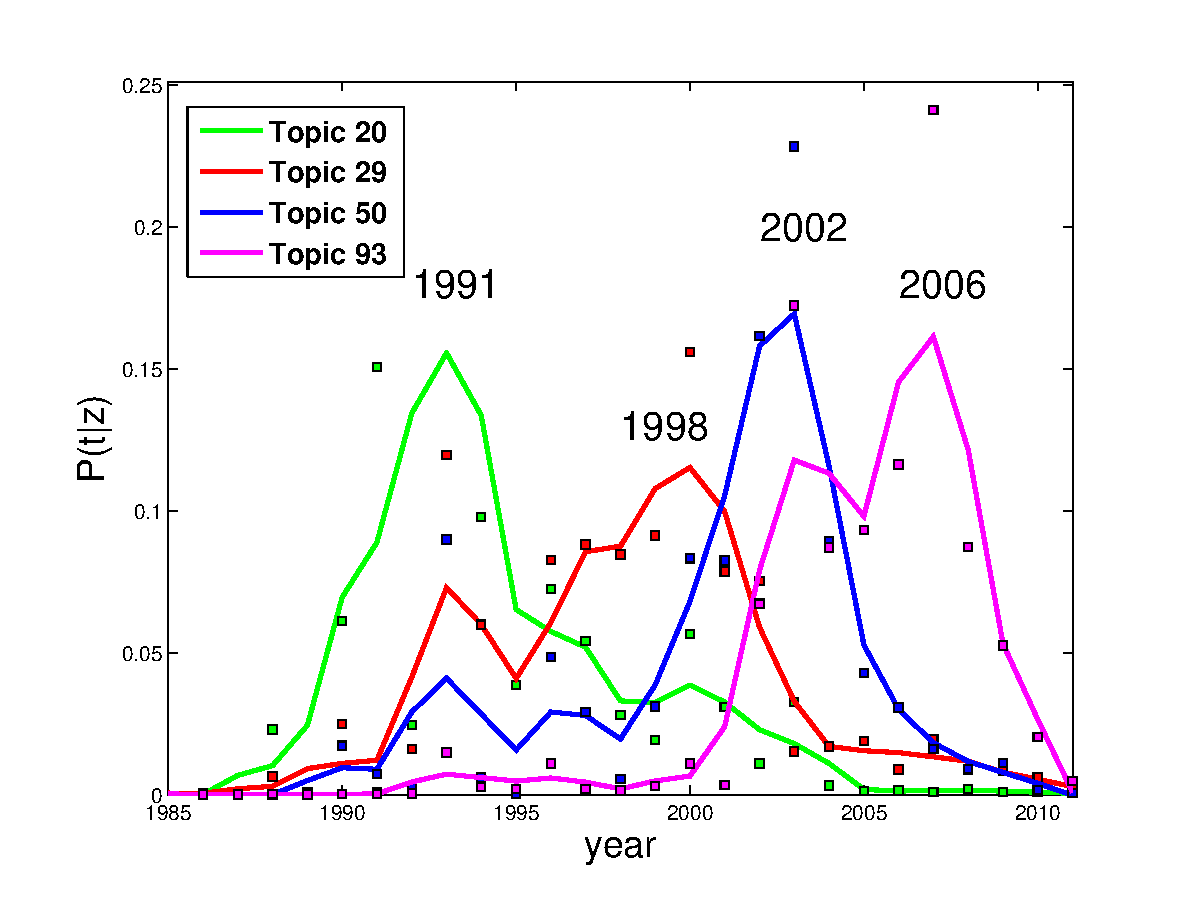
\includegraphics[scale= .6]{citation-lda/plot/smt_4topic_temporal}
    ~
    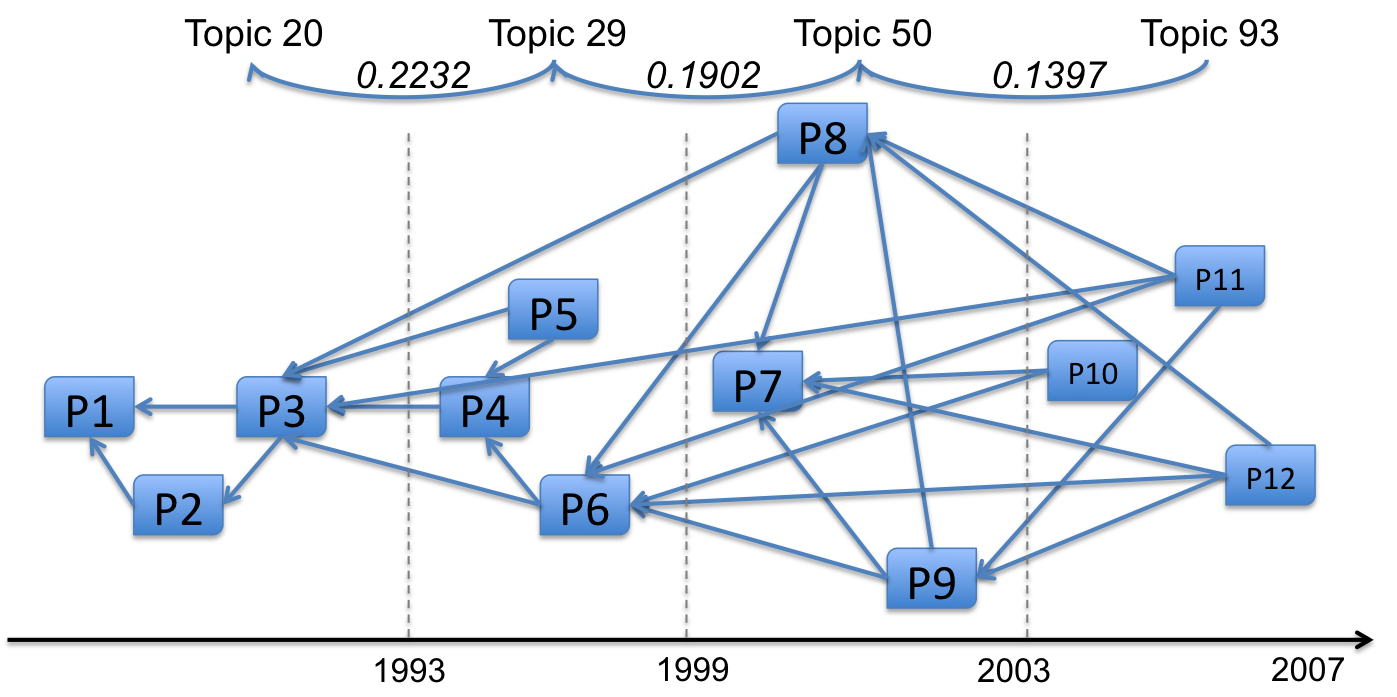
\includegraphics[scale= .45]{citation-lda/plot/smt_milestone_link}
  \end{center}
  \caption{Temporal Evolution in Topics of Theme SMT}\label{fig:smt_temporal}
\end{figure}

Specifically, Topic~20 began increasing its impact around early 90s, introducing
basic statistical methods to machine translation; Later, around 1998, its
popularity was shifted to Topic~29 which was specialized in subproblems such as
``decoding'', ``alignment'' and ``reordering'' in SMT; By 2002, however, Topic
50 emerged, and soon grew as the new dominant topic by proposing ``BLEU'' as the
standard evaluation metric and investigating ``discriminative methods'' such as
``minimum error rate training''; The current state of the art approach in SMT,
``phrase-based model'', accompanied by the raise of Topic~93, was actually built
on top of previous work, especially milestone papers of $P7$-$P9$ of Topic~50.

In \Cref{fig:smt_temporal}, citation links among milestone papers across topics
are illustrated, which clearly show the formation of topics through the ``stable
core set'' of milestone papers that \emph{get cited together}~(co-cited). More
importantly, it is evident that the ``co-citation'' of ``core'' papers is the
direct contributing factor in the dependency relation between two consecutive
topics.

\subsection{Model Selection \& Comparison Results}
\label{sec::citation_sec_model_selection}

We now discuss how to select the topic numbers for Citation-LDA and compare the
performance with Content-LDA on two metrics, namely, \emph{Forward Citation} and
\emph{Jounral Conditional Entropy}.

We investigate the conventional Content-LDA~\cite{blei2003latent} as our
baseline, using the title and abstract to represent the papers in both datasets.
In order to make the output of Content-LDA aligned with that of Citation-LDA, we
need to derive the missing \emph{topic-doc} distribution: the distribution over
papers (instead of tokens) for each topic.  As in our experiments, we assume
{$\Pr(d | k) \propto \Pr(k | d) \cdot \Pr(d)$} whereas {$\Pr(d)\propto |d|$}
with {\scriptsize $|d|$} being the document length for $d$.

\subsubsection{Evluation on Forward Citation for AAN}

We compute the \emph{topic forward citation} probability based on the topic
dependency~(\Cref{eq::citation_lda_citation_structure}) and expected topic
time~(\Cref{eq::citation_time3}).  In words, the forward citation probability
reflects the chance a topic \emph{cites} future topics that arise after
itself~(though it is impossible for a paper to cite a future paper).  We compute
the model's loss on topic $k$ by the topic \emph{future citation probability} ,
which is given by: {$l(k) = \sum\limits_{\tilde{k}, t(\tilde{k}) > t(k)} \Pr(k
\rightarrow \tilde{k} | k)$} for topic $k$. To assess the total \emph{loss for
Forward Citation} of a model, we define it as follows:

 $$\mathrm{Loss}_{FC} = \sum\limits_k \Pr(k) \cdot l(k)$$

\begin{table}[h!]
\caption{Loss on Forward Citation~(AAN)}
\label{tab::citation-fc}
\begin{center}
\begin{tabular}{|c|c|c|c|}
\hline
\#topic	&	20	&	100	&	200 \\
\hline\hline
Citation-LDA 	& 0.3148		&	\textbf{0.1917}	&	0.2488	\\
Content-LDA		& 0.3745		&	0.3816	&	0.3924	\\
\hline \hline
\end{tabular}
\end{center}
\end{table}

We show the evaluation based on \emph{Forward Citation} for AAN in
\Cref{tab::citation-fc}, from which we see: 1) Citation-LDA has better
performance on Forward Citation compared with Content-LDA and 2) 100 topics are
a good choice for AAN dataset.

\subsubsection{Evaluation on Journal Conditional Entropy for PMC}

As discussed before, the journal sources are fairly good ``coarse'' annotation
for topics in PMC. For topic $k$, we can derive the \emph{journal conditional
  distribution on topic $k$}, yielding the conditional entropy~\footnote{Entropy
$H(X) = - \sum\limits_{x} \Pr(x) \log \Pr(x)$}:  $$H(J | z) =
\sum\limits_{z=k} \Pr(z=k) \cdot H(J | z=k)$$ The $H(J | z)$ would have low
value if the journal labels and topic labels are \emph{consistent}, by which
we mean that for papers with the \emph{same topic label}~(in a probabilistic
sense), there is \emph{one journal label} being as dominant as possible,
ideally being purely the only journal label. Hence, we can compute the
\emph{loss for Journal Conditional Entropy} of a model as:

$$\mathrm{Loss}_{CE} = H(J|z)$$

\begin{table}[h!]
\caption{Loss on Journal Conditional Entropy~(PMC)}
\label{tab::citation-ce}
\begin{center}
\begin{tabular}{|c|c|c|c|c|}
\hline
\#topic	&	100	& 300 &	500	&	1000 \\
\hline\hline
Citation-LDA 	& 	3.5047	&	3.2144	&	\textbf{3.18729}	&	3.4118\\
Content-LDA		& 	4.2048	& 	4.2805	&	4.06496	&	4.4725\\
\hline \hline
\end{tabular}
\end{center}
\end{table}

Based on the journal conditional entropy on
topics~(\Cref{tab::citation-ce}), we again demonstrate the advantage of
Citation-LDA over Content-LDA: the topic formed in Citation-LDA is more
consistent with the ``journal labels'' than Content-LDA. In addition, we verify
that for PMC dataset, 500 topics might be a reasonable choice.


\section{Notes and Conclusion}\label{sec::citation-conclusion}

In this chapter, we proposed a novel approach for analyzing research theme
evolution of scientific literature data where citation links are available.  1)
to discover research topics, which includes finding milestone papers, computing
topic temporal strength, and extracting keywords for topics; 2) to discover
theme evolution, which includes identifying topic importance, learning topic
dependency relation, and recognizing the evolution patterns.  These
computational components together enable us to understand evolution of research
themes by constructing the evolution graph.  In experiments, we investigated two
datasets, namely AAN and PMC from two domains, with extensive results showing
that our proposed model, Citation-LDA, which represents article paper as ``bag
of citations'' and model the generation of citation links within a probabilistic
framework, can effectively accomplish the tasks defined above, with the
performance better than Content-LDA.  Our proposed Citation-LDA, together with
the developed mining techniques, can be very useful to help researchers digest
literature quickly, thus speeding up scientific research discovery and
delivering very broad positive impact on the society.

In general, our model can also be applied to any graph data for tasks such as
network clustering and ranking, as well as modeling the evolution of network
generation, which we leave as future work directions.


\chapter{Blind Men and The Elephant: \\
  Thurstonian Pairwise Preference for Ranking in Crowdsourcing}\label{chp::tpp}
\section{Introduction}

Collecting reliable annotation at scale has been a critical issue in the
development of machine learning techniques. Crowdsourcing services make it
possible to collect huge amount of annotations from less trained crowd workers
in an inexpensive and efficient manner. The general philosophy of crowdsourcing
is that instead of collecting one single expert-annotated label for each
instance, multiple labels per example are collected from non-expert crowd
workers at low cost to infer the ground
truth~\cite{welinder2010multidimensional,whitehill2009whose}.

\subsection{Motivation}

In different tasks of learning, the form of labels can
be as simple as binary/pairwise judgements, but can also be structured and
complex.  An example of the latter case is a ranked list of documents with
respect to a query. \emph{Ranked lists} offer the most informative knowledge for
training and testing in various data mining and information retrieval tasks such
as \emph{learning to rank}~\cite{valizadegan2009learning,yue2007support}.
Nevertheless, unlike making binary or pairwise judgements, labeling complex
structures such as ranked lists by crowd workers is subject to large variance
and low efficiency. In order to generate a ranked list of $N$ items, a worker
needs to consider a number of $N!$ possibilities. Annotation in such a huge
labeling space is time consuming and uneconomic. Furthermore, the non-expert
nature of crowdsourcing workers makes it even more difficult to reach  consensus
on the ground-truth ranked lists than binary/pairwise judgements.

The fact that ranked lists are highly useful but hard to be directly annotated
motivates us to seek for alternative strategies.  Our idea is based upon a
metaphor in which we can only \emph{learn} what \emph{an elephant} is like
through \emph{a group of blind men}. Each one holds onto a different part, but
only one part, such as the side or the tusk. In the original story, they then
discuss their observations which leads to argument and complete disagreement.
However, a smarter treatment is to analysis all the observations and to find an
probable explanation that most fits. In this chapter, we implement such idea by
decomposing the task of labeling ranked lists into a series of smaller and
easier tasks: \textit{annotating pairwise preferences}, each of which requires a
worker to compare only a pair of items out of the entire set.  In addition, the
pairwise judgements by crowd workers are more reliable and can be easily scaled
up. Pairs of items can be randomly generated out of the set and will be labeled
by multiple workers.  The goal is to infer the true \emph{ranked list} out of
the \emph{crowdsourced pairwise} annotations.

\subsection{Challenges}

Leveraging pairwise preferences to infer the full ranked list is promising but
also challenging. The key challenge comes from \emph{\underline{incomplete}} and
\emph{\underline{inconsistent}} annotations.

Pairwise preferences can be \emph{incomplete} due to time and budget
constraints. Not every two items are compared either directly or indirectly (For
items $A$, $B$ and $C$, an \textit{indirect} annotation of $A \succ B$ may be
obtained if \textit{direct} annotations of $A \succ C$ and $C \succ B$ have been
given). The available annotations can also be \emph{inconsistent}, resulting
from either the disagreements between multiple workers, or the intrinsic
uncertainty within one single worker. A common mistake of the latter case is
that one labels  $A \succ B, B \succ C, \mbox{ and } C \succ A$ at the same
time. The discussion below reveals a number of factors that lead to inconsistent
annotations:

\begin{itemize}
\item \emph{Query difficulty:}  More difficult queries, such as ambiguous and
  vague queries, demand more effort to interpret and to judge, making them
  intrinsically more prone to errors.
\item  {\emph{Worker expertise across domains:}} Different workers have
  different domain expertise; the same worker can also have varying domain
  knowledge across different task, making the quality of their labels vary
  accordingly. In practice, neither the task domain nor the worker's expertise
  is known apriori.
\item {\emph{Truthfulness of Workers:}} Truthfulness of workers is a prevailing
  issue in crowdsourcing tasks. Two typical adversarial groups are spammer
  workers and malicious workers: Spammers give random judgments and offer little
  information about the ranked lists;  Malicious workers, on the other hand,
  sabotage the utility of annotations by giving false preferences.
\end{itemize}

Identifying the sources of such incompleteness and inconsistency, and properly
modeling them, are critical to infer the true ranked list from the crowdsourced
pairwise annotations.

\subsection{Our Proposal}

We propose a novel generative model called ``Thurstonian Pairwise Preference''
(\tpp{}) to bind pairwise preferences of the crowd into rankings.  The key
modeling challenges that \tpp{} addresses are to resolve the inevitable
incompleteness and inconsistency of judgements, as well as to model variable
query difficulty and different labeling quality resulting from workers' domain
expertise and truthfulness.

\tpp{} is built on top of the Thurstonian Ranking Model (\trm{})
\cite{thurstone1927law}, which takes noisy ranked lists of items as observations
and estimates the true rankings. When applied to crowdsourcing, \trm{} models
the generation of the noisy ranked lists annotated by crowd workers, taking
variable query difficulty into account. It infers the relevance score of each
item to form the ranked list. In contrast to \trm{}, the observations of \tpp{}
are pairwise preferences.  Specifically, \tpp{} naturally simulates the
generative process of incomplete pairwise annotations, and seamlessly integrates
a worker-aware layer with the original query-aware layer to model the
inconsistency of the labeling process.  The advantage of \tpp{} is that it does
not require full rankings as observations, and pairwise preferences can be
efficiently labeled at scale.

While there have been earlier research efforts on (pairwise) ranking aggregation
with similar goals, most of them investigated a ``non-crowd'' setting, or only a
subset of the above factors are taken into account~(See
\Cref{sec::tpp_related_work} for details). In sharp contrast, \textsc{Tpp}
provides a unified and principled strategy to handle various influential
factors, which  effectively binds pairwise preferences of the crowd into
rankings.

\noindent \textbf{Organization.} We briefly introduce the original Thurstonian
Ranking Model in \Cref{sec::tpp_trm}, and present our proposed Thurstonian
Pairwise Preference model (\tpp{}) in \Cref{sec::tpp_tpp}. The inference of
\tpp{} is given in \Cref{sec::tpp_infer}. We provide the experimental study in
\Cref{sec::tpp_exp}, review related work in \Cref{sec::tpp_related_work} and
conclude our study in \Cref{sec::tpp_conclude}.

\section{Thurstonian Ranking Model} \label{sec::tpp_trm}

The original Thurstonian ranking model (\textsc{Trm})~\cite{thurstone1927law} is
devised for analyzing ordinal data.  Suppose in a ranking annotation task, $K$
workers $\{t_k\}_{k=1}^{K}$ are given $Q$ queries $\{q_l\}_{l=1}^Q$ and $D$
documents $\{d_i\}_{i=1}^D$.  It is postulated that the optimal ranked
list\footnote{a permutation of documents} for query $q_l$ is determined by the
\emph{ground truth relevance score} $s_{l,i}$ of each document $d_i$.
Precisely, the larger the value of $s_{l,i}$, the higher rank is assigned to
$d_i$.  Each worker $t_k$ produces a ranked list $\sigma_l^{(k)}$ by ordering
documents according to his \emph{perceived relevance scores} $s_{l,i}^{(k)}$,
which are assumed to be Gaussian distributed: $s_{l,i}^{(k)} \sim
\mathrm{N}(s_{l,i}, \delta_l^2)$.  The variance $\delta_l^2$ quantifies the
\emph{query difficulty} of $q_l$: $\delta_l^2$ is larger for more difficult
query, and the perceived score can deviate more from the ground truth score.

\begin{figure}[h!]
	\begin{center}
		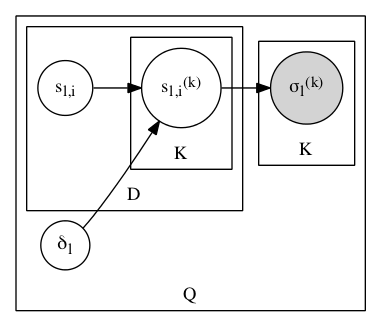
\includegraphics[width=0.4\textwidth]{crowd-thurstonian/figure/thurstonian.png}
		\caption{Plate notation for \textsc{Trm}} \label{fig::thurstonian}
		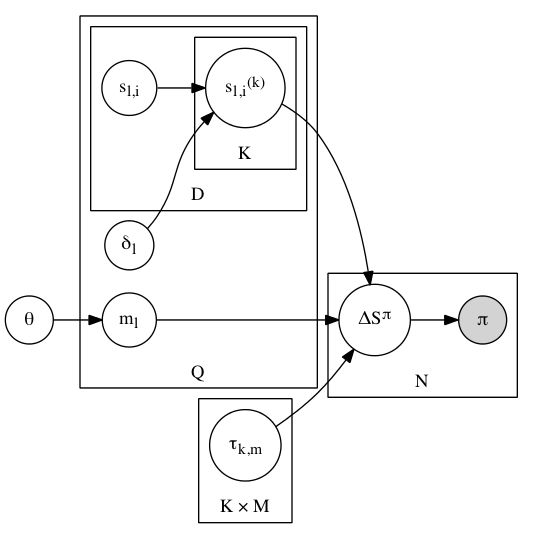
\includegraphics[width=0.5\textwidth]{crowd-thurstonian/figure/tpp.png}
		\caption{Plate notation for \textsc{Tpp}} \label{fig::tpp}
	\end{center}
\end{figure}

The plate notation of the above generative process is given in
\Cref{fig::thurstonian}.  With the workers' annotated rankings
$\{\sigma_l^{(k)}\}$ given as observations, the goal of \textsc{Trm} is to infer
$\{s_{l,i}\}$ as well as $\{\delta_l^2\}$.  Algorithmic development for
inference previously investigated includes maximum likelihood
estimation~\cite{bockenholt1993applications} and Bayesian
inference~\cite{yao1999bayesian}. A derivation of the maximum likelihood
estimation is given in \Cref{app::trm}.

\section{Thurstonian Pairwise Preference} \label{sec::tpp_tpp}

\begin{table}[h!]
\caption{Summary of Notations} \label{tab::tpp_notation}
\begin{center}
\begin{tabular}{ll}
\hline
Notation 	& Explanation \\
\hline
\hline
$t_k$, $q_l$, $d_i$					&
      worker $t_k$, query $q_l$ and document $d_i$ \\
$s_{l,i}$  							    &
      ground truth relevance score of $d_i$ \emph{w.r.t.} $q_l$\\
$\delta_l^2$ 						    &
      the difficulty of query $q_l$\\
$m_l$								        &
      the domain of query $q_l$ \\
\multirow{2}{*}{$\vect{\theta}=(\theta_1, \dots ,\theta_M)^T$}		&
      the distribution of query domains,      \\                  &
      $m_l \sim \mathrm{Mult}(\vect{\theta})$ \\
\multirow{2}{*}{$\tau_{k,m}$}		                                  &
      worker $t_k$'s expertise \& truthfulness \\                 &
      on domain $m$\\
$s_{l,i}^{(k)}$ 						&
      worker $t_k$'s perceived score of $d_i$ \emph{w.r.t.} $q_l$\\
\multirow{2}{*}{$\pi=\langle k,l,i_1,i_2 \rangle$} 	              &
      pairwise preference $\pi$: $t_k$ prefers document \\        &
      $d_{i_1}$ to document $d_{i_2}$ \emph{w.r.t.} $q_l$\\
\multirow{2}{*}{$\tilde{s}_{i_1}^{\pi}, \tilde{s}_{i_2}^{\pi}$}	  &
      noisy scores of $d_{i_1}$ and $d_{i_2}$ to determine \\     &
      pairwise preference $\pi$\\
$\Delta s^{\pi}$ 					                                        &
      noisy score difference
      $\Delta s^{\pi} = \tilde{s}_{i_1}^{\pi} - \tilde{s}_{i_2}^{\pi}$  \\
$\mathbf{\Theta} = \{ s_{l,i}, \delta_l^2, \theta_m, \tau_{k,m}\}$ 	&
      model parameters \\
$\mathbf{Z} = \{m_l, s_{l,i}^{(k)}\}$ 							              	&
      latent variables of interest \\
$\mathbf{V} = \{\Delta s^{\pi}\}$									                  &
      auxiliary latent variables \\
$\mathbf{D} = \{\pi\}$											                        &
      observations \\
\hline
\end{tabular}
\end{center}
\end{table}%

\trm{}  specifies the generation of ranked lists in a crowdsourced setting, with
variable query difficulty taken into account. However, the difficulty in
obtaining annotated \emph{ranked lists} makes it hardly applicable in practice.
We propose a novel generative model called ``Thurstonian Pairwise Preference''
(\tpp{}), which extends \trm{} to accommodate \emph{pairwise preferences} as
observations. Meanwhile, \tpp{} seamlessly integrates a \emph{worker-aware}
layer with the original query-aware layer to incorporate workers' variable
expertise across different domains and their truthfulness, which explains the
generation of the inconsistent pairwise preferences at modeling time.

The plate notation of \textsc{Tpp} is given in \Cref{fig::tpp}. The
notations used throughout this chapter are summarized in
\Cref{tab::tpp_notation}. Suppose worker $t_k$ compares documents $d_{i_1}$ and
$d_{i_2}$ \emph{w.r.t.} query $q_l$. The pairwise preference $\pi$ is either
$t_k$ prefers $d_{i_1}$ to $d_{i_2}$, denoted by $\langle k, l, i_1, i_2
\rangle$, or $\pi = \langle k, l, i_2, i_1 \rangle$ if $t_k$ prefers
$d_{i_2}$\footnote{We adopt the assumption made in \trm{} that no ties exist in
rankings. However, if two documents are indeed equally relevant, the workers
shall randomly prefers either one, and the ground truth relevance scores of
the two documents would be close.}. The preference depends on query
difficulty, as well as the domain expertise and truthfulness of the worker.

\tpp{} first generates the workers' perceived scores in the same way as \trm{}
does. Then it introduces a worker-aware layer to simulate the generation of
pairwise annotations, which involves a delicate modeling of query domains.  We
assume there are $M$ domains. For query $q_l$, its domain $m_l$ is drawn from a
multinomial distribution: $m_l \sim \mathrm{Mult}(\vect{\theta})$. In order to
generate the pairwise preference $\pi$, worker $t_k$ generates two noisy scores
$\tilde{s}_{i_1}^{\pi}$ and $\tilde{s}_{i_2}^\pi$, which are Guassian
distributed: $\tilde{s}_{i_1}^{\pi} \sim \mathrm{N}(\mathrm{sgn}(\tau_{k,m_l})
  s_{l,i_1}^{(k)}, \tau_{k,m_l}^{-2})$ and $\tilde{s}_{i_2}^{\pi} \sim
  \mathrm{N}(\mathrm{sgn}(\tau_{k,m_l}) s_{l,i_2}^{(k)},
\tau_{k,m_l}^{-2})$.\footnote{$\mathrm{sgn}(x) =\left\{  \begin{array}{ll} 1 &
\textrm{if}~x > 0 \\ -1 & \textrm{otherwise}\end{array} \right.$} The parameter
$\tau_{k,m}$ encodes worker $t_k$'s expertise and truthfulness on domain $m$.
Specifically, the sign of $\tau_{k,m}$ indicates whether worker $t_k$ is
truthful or malicious on domain $m$. A malicious worker would have a negative
$\tau_{k,m}$, giving false preferences by ``flipping'' his perceived scores.
The absolute value of $\tau_{k,m}$ measures the expertise of $t_k$ on $m$: a
larger $|\tau_{k,m}|$ means a smaller variance of the noisy score, \ie, $t_k$ is
more knowledgeable on $m$; for a very small $|\tau_{k,m}|$, the noisy score is
nearly uniformly distributed, implying $t_k$ likely to be a spammer. Given the
noisy scores $\tilde{s}_{i_1}^{\pi}$ and $\tilde{s}_{i_2}^\pi$, the pairwise
preference is uniquely determined: $\pi = \langle k, l, i_1, i_2 \rangle$ if
$\tilde{s}_{i_1}^{\pi} - \tilde{s}_{i_2}^{\pi}  \geq 0$ and vice versa.  We
define the \emph{noisy score difference} in this case as:
\begin{equation}
\Delta s^\pi =  \tilde{s}_{i_1}^{\pi} - \tilde{s}_{i_2}^{\pi}
\label{eq::tpp_deltas}
\end{equation}
and thus $\P(\pi = \langle k, l, i_1, i_2 \rangle) = \P(\Delta s^\pi \geq 0)$.

The generative process of \textsc{Tpp} is summarized as follows:

\begin{itemize}
\item \textbf{Generate Perceived Scores:} Generate worker $t_k$'s perceived
  score of document $d_i$ \emph{w.r.t.} query $q_l$:  $s_{l,i}^{(k)} \sim
  \mathrm{N}(s_{l,i}, \delta_l^2)$
\item \textbf{Generate Query Domains:} For query $q_l$, draw its domain: $m_l
  \sim \mathrm{Mult}(\vect{\theta})$.
\item \textbf{Generate Noisy Scores:} To compare two documents $d_{i_1}$ and
  $d_{i_2}$, worker $t_k$ generate noisy scores $\tilde{s}_{i_1}^{\pi}$ and
  $\tilde{s}_{i_2}^{\pi}$.
    \begin{equation}
    \tilde{s}_{i_j}^{\pi} \sim \mathrm{N}(
                        \mathrm{sgn}(\tau_{k,m_l}) s_{l,i_j}^{(k)},
                        \tau_{k,m_l}^{-2}) ~(j=1,2)
                        \label{eq::tpp_ns_gen}
    \end{equation}
\item \textbf{Generate Pairwise Preferences:} The pairwise preference $\pi$ is
  determined by the noisy score difference: $\pi=\langle k, l, i_1, i_2 \rangle$
  if $\Delta s^\pi  = \tilde{s}_{i_1}^{\pi} - \tilde{s}_{i_2}^{\pi}  \geq 0$,
  and $\pi=\langle k, l, i_2, i_1 \rangle$ if $\Delta s^\pi < 0$.
\end{itemize}

\begin{figure}[h!]
  \hspace{2.5cm}
		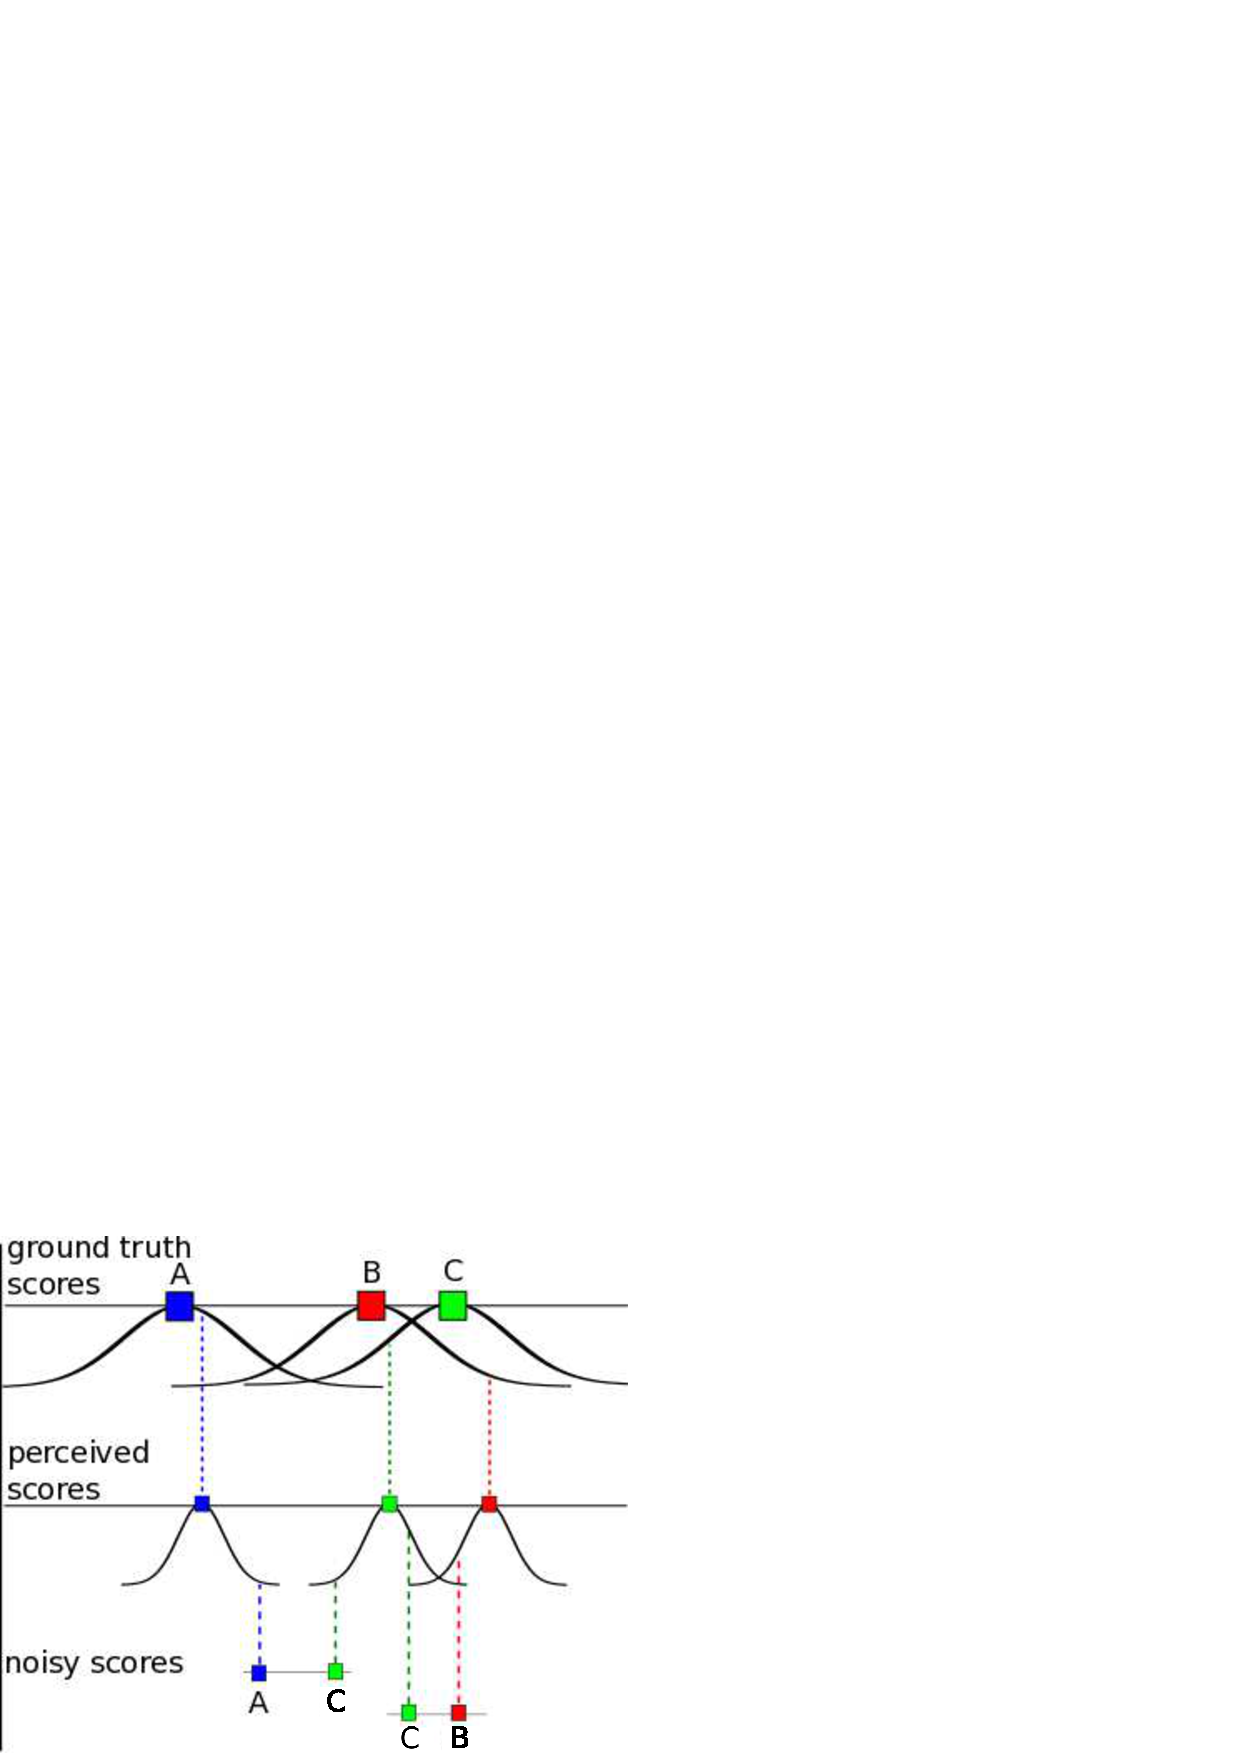
\includegraphics[scale=0.8,trim={0 14cm 0 6cm},clip]{crowd-thurstonian/figure/gaussian.pdf}
    \caption{An Illustration Example of \tpp{}: The generation of two pairwise
    preferences by a crowd worker for a given query} \label{fig::gaussian}
    \caption*{The true ranking is determined by the  ground truth scores of each
      document. The perceived score of each document is Gaussian distributed
      based on the true score and the query difficulty. Each time a worker is
      asked to compare a pair of documents, The perceived scores, together with
      the domain expertise and truthfulness of the worker, specify another two
      Gaussian distributions from which the noisy scores are drawn. The pairwise
      preference is given accordingly. The worker is truthful in this example.}
\end{figure}

\Cref{fig::gaussian} illustrates the generation of two pairwise
preferences by a crowd worker for a given query. The ground truth scores for
three documents $A,B,C$ imply the true ranking to be $A \prec B \prec C$. The
worker's perceived scores deviate from the ground truth scores due to query
difficulty. In fact, the perceived scores imply $A \prec C \prec B$, which
contradicts with the true ranking.  We further assume that the worker is
truthful and has reasonable domain knowledge (This example does not include the
generation of query domains for the sake of clarity). The worker generates noisy
scores which are close to his perceived scores, and gives pairwise
preferences~($A \prec C$, $C \prec B$) accordingly.  It is worth noting that a
pair of noisy scores are drawn each time a worker judges a pair of documents.
Thus \textsc{Tpp} respects {intra-worker inconsistency} as well as {inter-worker
inconsistency}.


\section{Inference}  \label{sec::tpp_infer}

The model parameters $\mathbf{\Theta} = \{ s_{l,i}, \delta_l^2, \theta_m,
\tau_{k,m}\}$ are learned by Maximum Likelihood Estimation (MLE) with the
Expectation-Maximization (E-M)~\cite{dempster1977maximum} algorithm.  The
posterior distribution of the \textit{latent variables of interest} $\mathbf{Z}
= \{m_l, s_{l,i}^{(k)}\}$ given the observations $\mathbf{D} = \{\pi\}$ is
approximated via alternate sampling of $\mathbf{Z}$ and the \textit{auxiliary
latent variables} $\mathbf{V}  = \{\Delta s^{\pi}\}$.  The inference algorithm
of \tpp{} is summarized in \Cref{alg::tpp}.

\begin{algorithm}[h!]
\caption{Inference of \tpp{}}\label{alg::tpp}
	\KwIn{Pairwise preferences $\mathbf{D}$}
	\KwOut{Model parameters $\mathbf{\Theta}$}
	Initialize $\mathbf{V}, \mathbf{Z}, \mathbf{\Theta}$\;
	\While{convergence criteria not met}{
		(E-step) Sample the posterior distribution of $\mathbf{V}$ and $\mathbf{Z}$\;
		(M-step) Update $\mathbf{\Theta}$\;
		Model rescaling\;
	}
\end{algorithm}

\subsection{Model Parametrization}
The pairwise preference $\pi = \langle k, l, i_1, i_2 \rangle$ between two
documents $d_{i_1}$ and $d_{i_2}$ hinges on $\Delta s^\pi =
\tilde{s}_{i_1}^{\pi} - \tilde{s}_{i_2}^{\pi}$.  We introduce \textit{auxiliary
latent variables} $\mathbf{V}  = \{\Delta s^{\pi}\}$  to parameterize
\textsc{Tpp}.

Our results rely on the following lemma of (truncated) Gaussian distribution,
the proof of which can be found in \cite{chopin2011fast}):
\begin{lem}\label{lem::gaussian_diff}
If $x_1$ and $x_2$ are independently sampled from $x_i \sim \mathrm{N}(\mu_i,
\sigma^2),~i=\{1,2\}$,  then we have
\begin{itemize}
\item[(a)] $x_1 - x_2 \sim \mathrm{N}(\mu_1 - \mu_2, 2\sigma^2)$
  and  $\P(x_1 - x_2 \geq 0) = Q(-\frac{\mu_1-\mu_2}{\sqrt{2}\sigma})$, where
  $Q(\cdot)$ denotes the tail probability of the standard normal distribution:
  $Q(s) \defeq \Pr(x \geq s)$, $x\sim \mathrm{N}(0, 1)$.
\item[(b)] $x_1 - x_2 | x_1 - x_2 \geq 0 \sim \mathrm{TN}_0^{\infty}(\mu_1 -
  \mu_2, 2\sigma^2)$, where $\mathrm{TN}_a^{b}(m, s^2) ~(a<b, a, b \in
  \mathbb{R} \cup \{\pm \infty\})$ is the truncated Gaussian distribution
  bounded by interval $(a, b)$ with the embedded Gaussian distribution being
  $\mathrm{N}(m, s^2)$.
\qed
\end{itemize}
\end{lem}

Given \Cref{eq::tpp_deltas,eq::tpp_ns_gen}, it follows from
\Cref{lem::gaussian_diff}(a) that the auxiliary latent variable $\Delta
s^\pi$ follows the truncated Gaussian distribution:
\begin{flalign}
   \qquad \tilde{s}^\pi_{i_1} - \tilde{s}^\pi_{i_2} |
  \tau_{k,m_l}, s_{l,i_1}^{(k)}, s_{l,i_2}^{(k)}
   \sim \mathrm{N}\left(\mathrm{sgn}(\tau_{k,m_l})
    ( s_{l,i_1}^{(k)} -  s_{l,i_2}^{(k)}), 2\tau_{k,m_l}^{-2} \right)
  \label{eq::tpp_ds_dist}
\end{flalign}

and we have

\begin{flalign}
\P(\Delta s^\pi \geq 0 | \tau_{k,m_l}, s_{l,i_1}^{(k)}, s_{l,i_2}^{(k)}) =
    \mathrm{Q}\left(-\frac{\tau_{k,m_l}}{\sqrt{2}}
    ( s_{l,i_1}^{(k)} -  s_{l,i_2}^{(k)})\right) \label{eq::tpp_q_func}
\end{flalign}

In view of the above results, the joint probability of $\mathbf{D,Z,V}$ can be
factorized as:

\begin{align}
  &&&   \P(\mathbf{D, Z, V}| \mathbf{\Theta}) =
    \P(\mathbf{Z} | \mathbf{\Theta})
    \P(\mathbf{V} | \mathbf{Z})
    \P(\mathbf{D} | \mathbf{V}) \nonumber \\
  &&=&  \prod\limits_{l} \P_{\mathtt{Mult}}(m_l | \vect{\theta}) ~\cdot~
				\prod\limits_{k,l,i}
          \P_{\mathtt{N}}(s_{l,i}^{(k)} | s_{l,i}, \delta_l^2) \nonumber \\
  &&&   \prod\limits_{\pi=\langle k,l,i_1,i_2\rangle \in \mathbf{D}}
        \left(\P_{\mathtt{N}}\left(\Delta s^\pi | \mathrm{sgn}(\tau_{k,m_l})
            ( s_{l,i_1}^{(k)} -  s_{l,i_2}^{(k)}),
            2\tau_{k,m_l}^{-2}\right) \right.  \nonumber \\
  &&&   \prod\limits_{\pi=\langle k,l,i_1,i_2\rangle \in \mathbf{D}}
					  \mathbf{1}(\Delta s^\pi \geq 0 )
  \label{eq::tpp_join_alt}
\end{align}

Integrating out $\mathbf{V}$, we get the joint probability of the observations
$\mathbf{D} = \{\pi\}$ and the latent variables of interest $\mathbf{Z} = \{m_l,
s_{l,i}^{(k)}\}$:

\begin{align}
  & \P(\mathbf{D, Z}| \mathbf{\Theta}) = \int_{\mathbf{V}}
      \P(\mathbf{D, Z, V}| \mathbf{\Theta})~ \d \mathbf{V}\nonumber \\
  =&  \prod\limits_{l} \P_{\mathtt{Mult}}(m_l | \vect{\theta}) ~\cdot~
			    \prod\limits_{k,l,i}
          \P_{\mathtt{N}}(s_{l,i}^{(k)} | s_{l,i}, \delta_l^2) \nonumber\\
  &	\prod\limits_{\pi = \langle k,l,i_1,i_2\rangle \in \mathbf{D}}
          \mathrm{Q}\left(-\frac{\tau_{k,m_l}}{\sqrt{2}}
          ( s_{l,i_1}^{(k)} -  s_{l,i_2}^{(k)})\right)
  \label{eq::tpp_join}
\end{align}

The model parameters $\mathbf{\Theta} = \{ s_{l,i}, \delta_l^2, \theta_m,
\tau_{k,m}\}$ are learned by optimizing the log likelihood $\mathbf{\Theta} =
\argmax_{\mathbf{\Theta}} \ln \P(\mathbf{D | \Theta})$ with the E-M algorithm.
At the $t$-th iteration, the posterior distribution of $\mathbf{Z |
D,\Theta}^{(t)}$ is computed (E-step), followed by the model update, i.e.
maximizing the expected joint log likelihood: $\mathbf{\Theta}^{(t+1)} =
\argmax_\mathbf{\Theta} \mathcal{Q}(\mathbf{\Theta}; \mathbf{\Theta}^{(t)})$
(M-step), where

\begin{equation}
\mathcal{Q}(\mathbf{\Theta}; \mathbf{\Theta}^{(t)}) =
  \E_{\mathbf{Z | D,\Theta}^{(t)}}[\ln \P(\mathbf{D,Z | \Theta})]
\end{equation}

\subsection{Posterior Sampling}

The analytic calculation of $\mathcal{Q}(\mathbf{\Theta};
\mathbf{\Theta}^{(t)})$ is impossible due to the intractability of $\P(\mathbf{Z
| D, \Theta})$. Instead, we approximate the posterior distribution by sampling.
Nevertheless, sampling $\mathbf{Z}$ from $\P(\mathbf{Z | D, \Theta})$ is still
difficult because we cannot effectively integrate over \Cref{eq::tpp_join} to
obtain the distribution of $s_{l,i}^{(k)} | \mathbf{Z} \setminus
\{s_{l,i}^{(k)}\},\mathbf{D,\Theta}$.  Therefore, we reintroduce the auxiliary
latent variables $\mathbf{V}$. A blocked Gibbs sampler
\cite{geman1984stochastic} is applied to sample $\mathbf{V}$ and $\mathbf{Z}$.
Each block of variables, \ie, query domains $\{m_l\}$, perceived scores
$\{s_{l,i}^{(k)}\}$, and noisy score differences $\{\Delta s^\pi\}$, are sampled
in sequence.

\subsubsection{Sample Query Domain $m_l$} It follows from
\Cref{eq::tpp_join_alt} that the posterior distribution of the domain
$m_{l^*}$ for a query $l^*$ is given by the following multinomial distribution:

\begin{align}
& \P(m_{l^*} = m^* |
  \mathbf{D}, \mathbf{Z}\setminus \{ m_{l^*}\}, \mathbf{V}, \mathbf{\Theta})
  \label{eq::tpp_m} \\
\propto~ &  \theta_{m^*}
  \prod\limits_{\substack{\pi = \langle k,l,i_1,i_2\rangle \in \mathbf{D}
    \\ l = l^*}}
  \P_{\mathtt{N}}\left(\Delta s^\pi |
    \mathrm{sgn}(\tau_{k,m^*}) ( s_{l^*,i_1}^{(k)} -  s_{l^*,i_2}^{(k)}),
                2\tau_{k,m^*}^{-2}\right) \nonumber
\end{align}

Note that there is no coupling (inter-dependency) among $\{m_l\}$, and the
multinomial sampling can be accelerated with parallel implementation.

\subsubsection{Sample Perceived Score $s_{l,i}^{(k)}$}
It follows from \Cref{eq::tpp_join_alt} that the posterior distribution for the
perceived score is given by:
\begin{align}
& \P(s_{l^*,i^*}^{(k^*)} = s^* | \mathbf{D},
    \mathbf{Z}\setminus \{ s_{l^*,i^*}^{(k^*)} \}, \mathbf{V}, \mathbf{\Theta})
    \nonumber \\
\propto~ & \P_{\mathtt{N}}(s^* | s_{l^*,i^*}, \delta_{{l^*}}^2)
  \label{eq::tpp_s}\\
& \prod\limits_{\pi = \langle k^*,l^*,i^*,i\rangle \in \mathbf{D}}
    \P_{\mathtt{N}}(\Delta s^\pi |
      \mathrm{sgn}(\tau_{k^*,m_{l^*}}) ( s^* - s_{l^*,i}^{(k^*)}),
      2\tau_{k^*,m_{l^*}}^{-2}) \nonumber \\
& \prod\limits_{\pi = \langle k^*,l^*,i,i^*\rangle \in \mathbf{D}}
		\P_{\mathtt{N}}(\Delta s^\pi |
      \mathrm{sgn}(\tau_{k^*,m_{l^*}}) ( s_{l^*,i}^{(k^*)} - s^*),
      2\tau_{k^*,m_{l^*}}^{-2}) \nonumber
\end{align}

To derive the sampling rule for perceived score $s_{l,i}^{(k)}$, we employ the
following lemma that an exponential-family distribution is uniquely determined
by its sufficient statistics and natural parameters \cite{stuart1968advanced}:

\begin{lem}\label{lem::exp_dist}
If $\P(x)$ is a valid distribution and $\P(x) \propto \exp(c_1 x + c_2 x^2)$,
then $x \sim \mathrm{N}(- \frac{c_1}{2c_2}, -\frac{1}{2c_2})$
\qed
\end{lem}
And it follows immediately that:

\begin{equation}\label{eq::tpp_sps}
s_{l^*,i^*}^{(k^*)} \sim \mathrm{N}(\frac{a_1}{a_2}, \frac{1}{a_2})
\end{equation}

where

\begin{flalign}
a_1 &= \frac{1}{\delta^2_{l^*}} s_{l^*,i^*} \label{eq::tpp_a1}\\
	  &+ \frac{1}{2\tau_{k^*,m_{l^*}}^{-2}}
        \left( \sum\limits_{\substack{i \\
                          \pi = \langle k^*,l^*,i^*,i\rangle \in \mathbf{D}} }
              s_{l^*,i}^{(k^*)} + \mathrm{sgn}(\tau_{k^*,m_{l^*}})  \Delta s^\pi
        \right)  \nonumber \\
	  &+ \frac{1}{2\tau_{k^*,m_{l^*}}^{-2}}
        \left( \sum\limits_{\substack{i \\
                          \pi = \langle k^*,l^*,i,i^*\rangle \in \mathbf{D}} }
              s_{l^*,i}^{(k^*)} - \mathrm{sgn}(\tau_{k^*,m_{l^*}})  \Delta s^\pi
        \right) \nonumber\\
a_2 &= \frac{1}{\delta^2_{l^*}} + \frac{1}{2\tau_{k^*,m_{l^*}}^{-2}}
  \left(\sum\limits_{\substack{i \\
                      \langle k^*,l^*,i^*,i\rangle \in \mathbf{D}} }
        1 +
        \sum\limits_{\substack{i \\
                      \langle k^*,l^*,i,i^*\rangle \in \mathbf{D}} }
        1\right) \label{eq::tpp_a2}
\end{flalign}

\noindent\emph{\underline{Intuitive Interpretation}.} Here is an intuitive
interpretation of the above calculation which provides more insights into the
behaviors of \textsc{Tpp}:

First, the mean value $\frac{a_1}{a_2}$ is a weighted average of three sources
of estimation:

\begin{itemize}
\item $s_{l^*,i^*}$, the ground truth relevance score~(1st term in
  \Cref{eq::tpp_a1}). It is discounted by the query difficulty $\delta^2_{l^*}$.
  The easier the query, the more it contributes to the perceived
  score $s_{l^*,i^*}^{(k^*)}$.
\item $\left(s_{l^*,i}^{(k^*)} + \mathrm{sgn}(\tau_{k^*,m_{l^*}})\Delta
  s^\pi\right)$ where $\pi = \langle k^*,l^*,i^*,i\rangle \in \mathbf{D}$, (2nd
  term in \Cref{eq::tpp_a1}). It corresponds to a pairwise preference $\pi$ when
  $t_{k^*}$ \textit{prefers} $d_{i^*}$ to the other document $d_{i}$.  It
  estimates $s_{l^*,i^*}^{(k^*)}$ by combining the perceived score
  $s_{l^*,i}^{(k^*)}$ of the less preferred document $d_i$ and the noisy score
  difference $\Delta s^\pi = \tilde{s}^\pi_{i^*} - \tilde{s}^\pi_{i}$ multiplied
  by the worker's truthfulness
  $\left(\mathrm{sgn}\left(\tau_{k^*,m_{l^*}}\right)\right)$.  This estimation
  is then weighted by the worker's domain expertise
  ($\frac{1}{2}\tau_{k^*,m_{l^*}}^{2}$).
\item The third source of estimation~(3rd term in \Cref{eq::tpp_a1}) corresponds
  to the case when $d_{i^*}$ is less preferred by $t_{k^*}$. The analysis is
  analogous to that of the 2nd term.
\end{itemize}

In addition, the variance $\frac{1}{a_2}$ in \Cref{eq::tpp_sps} is the harmonic
average of the query difficulty  $\delta^2_{l^*}$ and the worker's domain
expertise $2\tau_{k^*,m_{l^*}}^{-2}$, which determines the uncertainty of the
perceived score $s_{l^*,i^*}^{(k^*)}$. The sampled perceived scores are more
localized to the mean value $\frac{a_1}{a_2}$ with easier queries and more
knowledgeable workers.

\subsubsection{Sample Noisy Score Difference $\Delta s^\pi$} Denote the pairwise
preference by $\pi^* = \langle k^*, l^*,i_1^*,i_2^* \rangle$. It follows from
\Cref{eq::tpp_join_alt} that

\begin{align}
& \P( \Delta s^{\pi^*} = \Delta s^* | \mathbf{D}, \mathbf{Z},
    \mathbf{V}\setminus \{\Delta s^{\pi^*} \}, \mathbf{\Theta})
    \label{eq::tpp_ds}\\
\propto~ &  \P_{\mathtt{N}}\left( \Delta s^* | \mathrm{sgn}(\tau_{k^*,m_{l^*}})
      ( s_{l^*,i_1^*}^{(k^*)} - s_{l^*,i_2^*}^{(k^*)}),
      2\tau_{k^*,m_{l^*}}^{-2}\right)  \mathbf{1}(\Delta s^* \geq 0 ) \nonumber
\end{align}

By Lemma~\ref{lem::gaussian_diff}(b), the posterior distribution of $\Delta
s^{\pi^*}$ is a truncated Gaussian distribution:

\[
  \mathrm{TN}_0^\infty\left(\mathrm{sgn}(\tau_{k^*,m_{l^*}})
    (s_{l^*,i_1^*}^{(k^*)} - s_{l^*,i_2^*}^{(k^*)}),
    2\tau_{k^*,m_{l^*}}^{-2}\right)
\]

Efficient sampling from a truncated Gaussian distribution can be found in
\cite{chopin2011fast}.

With the above sampling rules, $\{m_l\}$, $\{s_{l,i}^{(k)}\}$, and $\{\Delta
s^\pi\}$ are sampled in blocks. After the burn-in period, samples of
$\mathbf{Z}$ are collected to approximate the posterior distribution
$\P(\mathbf{Z | D, \Theta})$ (samples of $\mathbf{V}$ are discarded).


\subsection{Model Updating}
The model parameters are updated by
\begin{align}
\Theta^{(t+1)} &=
  \argmax_\Theta \mathcal{Q}(\mathbf{\Theta}; \mathbf{\Theta}^{(t)}) \nonumber\\
\textrm{where}~
\mathcal{Q}(\mathbf{\Theta}; \mathbf{\Theta}^{(t)}) &=
  \E_{\mathbf{Z | D,\Theta}^{(t)}}[\ln \P(\mathbf{D,Z | \Theta})]
  \label{eq::tpp_elbo}
\end{align}
with the posterior distribution $\mathbf{Z | D,\Theta}^{(t)}$ approximated by blocked Gibbs sampling.

Optimization details are given in Appendix~\ref{app::mmu}. Closed forms are
obtained for the update of ground truth scores $\{s_{l,i}\}$, query difficulties
$\{\delta_{l}^{2}\}$, and the domain distribution $\{\theta_m\}$. (Inexact)
Newton's method is applied to update the domain expertise and truthfulness of
workers $\{\tau_{k,m}\}$.

\subsection{Identifiability}
Identifiability is a property which a model must satisfy in order for precise
inference to be possible. In plain words, it requires that different values of
the parameters must generate different probability distributions of the
observable variables.

For modeling rankings of documents, the extra degree of freedom of the model can
potentially lead to an arbitrary scaling of the ground truth scores (or
parameters), and thus must be carefully avoided.

One may observe that for the same collection of observations $\mathbf{D}$, the
following two models have the same likelihood $\P(\mathbf{D|\Theta_1}) =
\P(\mathbf{D|\Theta_2})$ for any global factor $\sigma > 0$ and query-level
biases $\{b_l\}$.\footnote{This can be verified by comparing $\int_\mathbf{Z}
\P(\mathbf{D, Z|\Theta})$ using \Cref{eq::tpp_join} for $\mathbf{\Theta =
\Theta_1}$ and $\mathbf{\Theta = \Theta_2}$.}

\begin{align}
\mathbf{\Theta_1} &= \{ s_{l,i}, \delta^2_l, \theta_m, \tau_{k,m}\} \nonumber \\
\mathbf{\Theta_2} &= \{ (s_{l,i}-b_l) / \sigma, \delta_l^2 / \sigma^2,
  \theta_m, \tau_{k,m} \sigma \}
\end{align}

Therefore, these two sets of parameters are {not identifiable}.

To cancel such extra freedom, we regularize the model by adding the following
two constraints:

\noindent\underline{\emph{Identification Conditions}}
\begin{empheq}[left=\empheqlbrace]{align}
\sum_l \delta_l^2 	&= 1 \label{eq::tpp_id1}\\
\min_i s_{l,i} 	 	&= 0, \forall l \label{eq::tpp_id2}
\end{empheq}

The constraints are imposed after the model update in each iteration.
Rescaling in this way keeps the model from undesired drifting and scaling.



\section{Experiments} \label{sec::tpp_exp}

In this section, we systematically evaluate the techniques presented in this
work on both synthetic and real-world datasets.  Code and datasets are
available at the following repository:
\url{https://github.com/dragonxlwang/crowd_thurstonian}

\subsection{Simulated Study}

\subsubsection{Datasets} In order to test the effectiveness of \tpp{} under
various scenarios, we generate synthetic datasets with the following parameter
settings.

The ground truth relevance scores of a list of documents
$\{s_{l,i}\}_{i=1,2,...}$ for  query $q_l$  are generated from a uniform
distribution $\mathcal{U}[0, 1]$. Two different lengths are investigated:
$5$~(\textsc{Doc5}) and $30$~(\textsc{Doc30}).  Query difficulty $\delta^2_l$ is
generated from a uniform distribution $\mathcal{U}[0, 0.1]$.  To characterize
the variable quality of answers given by crowd workers, we assume that worker
$t_k$'s expertise and truthfulness $\tau_{k,m}$ on domain $m$ falls into one of
the following categories:

\begin{itemize}
\item \textit{Expert}: $\tau_{k,m} = 10$
\item \textit{Average}: $\tau_{k,m} = 5$
\item \textit{Spammer}: $\tau_{k,m} = 1$
\item \textit{Malicious}: $\tau_{k,m} = -10$
\end{itemize}

Three demographic groups are formed by changing the distributions over these
four categories. Let $p$ denote the categorical distribution over
[\textit{expert, average, spammer, malicious}]:

\begin{itemize}
\item \textsc{Demo1}: $p = [0.2, 0.6, 0.1, 0.1]$. This group represents the most
  common case where average workers are dominant.
\item \textsc{Demo2}: $p = [0.2, 0.4, 0.3, 0.1]$. This group has a large
  proportion of spammers that can hurt the annotation quality.
\item \textsc{Demo3}: $p=[0.2, 0.4, 0.1, 0.3]$. The pairwise preferences given
  by this group can be overwhelmingly misleading due to the presence of too many
  malicious workers.
\end{itemize}

In order to simulate the incompleteness of annotations, which in real world
often depends on factors such as time and budget constraints, we introduce a
variable, \emph{sparsity ratio} (\textsc{Sr}), to control the probability that a
pair of documents is judged by a worker.  For example, if there are a list of
$30$ documents, and $\textsc{Sr} = 0.05$, each worker will judge $\frac{30\times
(30-1)}{2} \times 0.05 = 21.75$ randomly selected pairs.

Finally, the following $8$ datasets are generated. Each of them contains $10$
workers, $10$ query domains and $100$ queries:  \textsc{Doc5Sr1.0Demo1,
Doc5Sr0.5Demo1}, \textsc{Doc5Sr0.5Demo2}, \textsc{Doc5Sr0.5Demo3},
\textsc{Doc30Sr0.1Demo1}, \textsc{Doc30Sr0.05Demo1}, \textsc{Doc30Sr0.05Demo2}
and \textsc{Doc30Sr0.05Demo3}.

\subsubsection{Baselines}
We compare the performance of \textsc{Tpp} against the following four baselines:
\begin{itemize}
\item \textsc{TppUniDom}: \tpp{} without modeling query domains, \ie, all
  queries are treated as from one single domain.
\item \textsc{TppUniExp}: \tpp{} without modeling the domain
  expertise/truthfulness of workers, \ie, all workers have the same expertise
  and truthfulness for a given query domain: $\tau_{k_1,m} = \tau_{k_2, m} =
  \tau_m,$ $\forall k_1, k_2$.
\item \textsc{TppUniDiff}: \tpp{} with identical query difficulty, \ie, all
  queries are equally difficult: $\delta_l^2 = 1/Q,~ \forall l$ with some
  constant $Q$.
\item \textsc{CrowdBt}: \textsc{CrowdBt} \cite{chen2013pairwise} is proposed to
  infer the ground truth scores out of pairwise preferences, which extends the
  Bradley-Terry model by taking worker accuracy into consideration.
  Specifically, a ``worker-independent'' pairwise preference between $d_{i_1}$
  and $d_{i_2}$ for $q_l$ is drawn from a Bernoulli distribution. The
  probability of $d_{i_1} \succ d_{i_2}$ is computed by the Sigmoid function:

  \begin{align}
  \sigma( s_{l, i_1} - s_{l, i_2}) =
    \Big( 1 + \exp\big( -\left(s_{l, i_1} - s_{l, i_2}\right) \big) \Big)^{-1}
    \nonumber
  \end{align}

  Once the pairwise preference is drawn, each worker has a certain probability
  (accuracy) to report it truthfully or ``flip'' it. Compared with \tpp{},
  \textsc{CrowdBt} lacks the mechanism to model multiple query domains, thus
  incapable to characterize workers' domain-dependent expertise and
  truthfulness. Furthermore, it simplifies the generation of inconsistent
  annotations as solely a result from worker accuracy.
\end{itemize}

\begin{table*}[t]
\caption{Crowd Pairwise Preferences Binding Performance
          (Kendall's tau Distance)}
\label{tab::sim_binding}
\setlength\tabcolsep{1.5pt}
\begin{center}
\begin{tabular}{c|rl|rl|rl|rl|rl}
\hline \hline
Dataset	&	\multicolumn{2}{c|}{\textsc{Tpp}}
        &	\multicolumn{2}{|c|}{\textsc{TppUniDom}}
        & \multicolumn{2}{|c|}{\textsc{TppUniExp}}
        & \multicolumn{2}{|c}{\textsc{TppUniDiff}}
        & \multicolumn{2}{|c}{\textsc{CrowdBt}} \\ \hline \hline
\textsc{Doc5Sr1.0Demo1}		& $\mathbf{0.386}$	&	$\pm0.031$	&	$0.414$
        &	$\pm0.037$	&	$0.466$	&	$\pm0.023$	&	$0.402$	&	$\pm0.046$
				& $0.468$	&	$\pm0.047$\\
\textsc{Doc5Sr0.5Demo1} 	& $\mathbf{0.574}$	&	$\pm0.067$	&	$0.728$
        &	$\pm0.066$	&	$0.846$	&	$\pm0.080$	&	$0.628$	&	$\pm0.069$
			  & $0.856$	&	$\pm0.028$\\
\textsc{Doc5Sc0.5Demo2} 	& $\mathbf{0.734}$	&	$\pm0.021$	&	$0.852$
        &	$\pm0.033$	&	$0.940$	&	$\pm0.037$	&	$0.754$	&	$\pm0.047$
			  & $0.960$	&	$\pm0.041$\\
\textsc{Doc5Sr0.5Demo3} 	& $1.592$	&	$\pm0.237$	&	$1.760$	&	$\pm0.077$
        &	$2.550$	&	$\pm0.029$	&	$\mathbf{1.540}$	&	$\pm0.288$
			  & $2.990$	&	$\pm0.060$\\ \hline
\textsc{Doc30Sr0.1Demo1} 	& $\mathbf{22.442}$	&	$\pm1.238$	&	$25.636$
        & $\pm0.302$	&	$29.204$&	$\pm0.291$	&	$26.866$&	$\pm0.456$
			  & $24.420$	& $\pm0.906$\\
\textsc{Doc30Sr0.05Demo1} 	& $\mathbf{40.640}$	&	$\pm0.926$	&	$45.498$
        &	$\pm0.408$	&	$45.636$&	$\pm0.178$	&	$47.258$&	$\pm0.959$
			  & $48.820$	& $\pm2.161$\\
\textsc{Doc30Sr0.05Demo2} 	& $\mathbf{61.818}$	&	$\pm2.713$	&	$70.548$
        &	$\pm0.821$	&	$81.782$&	$\pm0.145$	&	$66.488$&	$\pm2.026$
			  & $104.500$	& $\pm2.469$\\
\textsc{Doc30Sr0.05Demo3} 	& $\mathbf{129.156}$	&	$\pm1.892$	&	$139.154$
        &	$\pm0.243$	&	$142.496$&	$\pm0.587$	&	$135.04$&	$\pm1.864$
			  & $153.390$	& $\pm1.031$ \\ \hline\hline
\end{tabular}
\end{center}
\end{table*}%

\subsubsection{Performance Studies}

We test all the methods on synthetic datasets under various parameter settings,
and report Kendall's tau distance~\cite{kendall1938new}  between the inferred
optimal ranking and the ground truth ranking.  Kendall's tau distance is often
used to measure the dissimilarity between two ranked
lists~\cite{klementiev2008unsupervised}, which is computed as the number of
discordant pairs of the two ranked lists. A pair of documents is discordant if
their relative order is reversed in the two rankings.  For example, suppose two
ranked lists of length $5$ are $d_1 \succ d_2 \succ d_3 \succ d_4 \succ d_5$ and
$d_3\succ d_4 \succ d_1 \succ d_2 \succ d_5$. There are in total
$\frac{5(5-1)}{2}=10$ pairs and $4$ of them are discordant: $\{d_1, d_3\}$,
$\{d_1, d_4\}$, $\{d_2, d_3\}$, $\{d_2, d_4\}$,  thus the Kendall's tau distance
is $4$.  A small Kendall's tau distance indicates good performance. We run each
method on every dataset $5$ times and report the mean and standard deviation in
\Cref{tab::sim_binding}.

\noindent\underline{\emph{Overall Performance.}} \textsc{Tpp} outperforms all
other methods in general (the only exception is on \textsc{Doc5Sr0.5Demo3},
where \textsc{TppUniDiff} gives the best result with a small margin).  Among the
three variants of \textsc{Tpp}, \textsc{TppUniExp} has the worst performance in
recovering the ground truth rankings. This justifies the importance of modeling
workers' domain expertise and truthfulness. Compared with \textsc{CrowdBt},
\textsc{Tpp} consistently behaves significantly better, implying that the
assumed generative process provides more flexibility in modeling and better
explains the generation of inconsistent annotations.

\noindent\underline{\emph{Performance on Different Demographic Groups.}}
Spammers and malicious workers have negative effects on all the methods. The
decrease in performance due to malicious workers is  more striking than that due
to spammers.  Nevertheless, the proposed \textsc{Tpp} is more robust in
resisting the attack from malicious workers than the baselines.  Specifically,
we observe that the Kendall's tau has increased by $88.516$ for \textsc{Tpp}
when changing the dataset from \textsc{Doc30Sr0.5Demo1} to
\textsc{Doc30r0.5Demo3}~\footnote{The maximal Kendall's tau distance for
\textsc{Doc30} is $\frac{30(30-1)}{2} = 435$.}, while this number is $93.656$
for \textsc{TppUniDom}, $96.860$ for \textsc{TppUniExp}, and $104.57$ for
\textsc{CrowdBt}. This demonstrates that \textsc{Tpp} does a better job in
recognizing adversarial workers.

\noindent\underline{\emph{Performance \wrt{} Sparsity Ratio.}} Sparser
annotations provide less evidence to infer the ground truth rankings.  It is
observed that the best performance on \textsc{Doc5Sr0.5Demo1}  ($0.574$) is
still much higher (and thus worse) than the worst performance on
\textsc{Doc5Sr1.0Demo1} ($0.468$).  Similar observations are obtained on the
\textsc{Doc30} datasets.

\subsubsection{Query Domain Prediction}

We investigate the  capability of \textsc{Tpp} in distinguishing between queries
from different domains.

\begin{figure}[h!]
	\centering
		\begin{subfigure}[b]{.5\linewidth}
      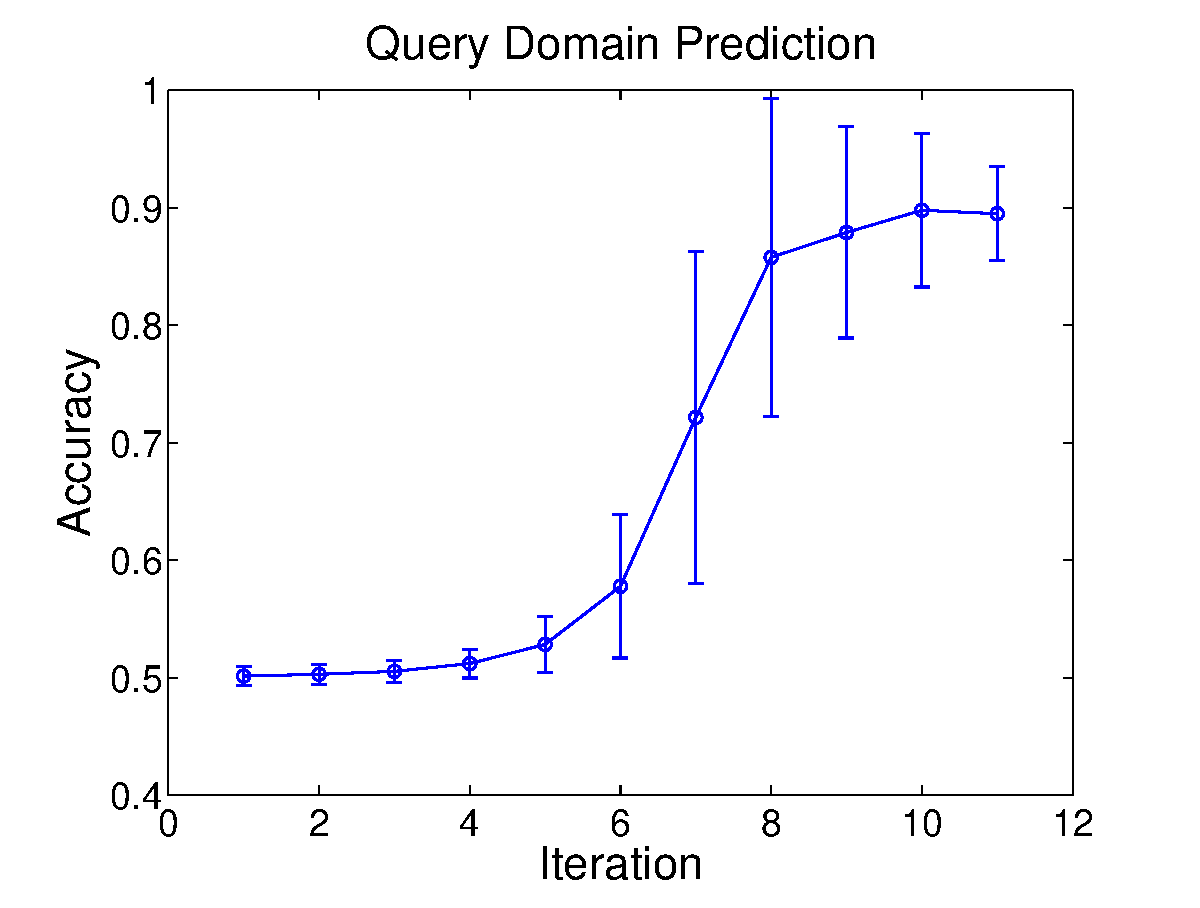
\includegraphics[width=1\textwidth]{crowd-thurstonian/figure/dp_acc.eps}
      \caption{Accuracy} \label{fig::dp_acc}
		\end{subfigure}
    ~
		\begin{subfigure}[b]{.5\linewidth}
      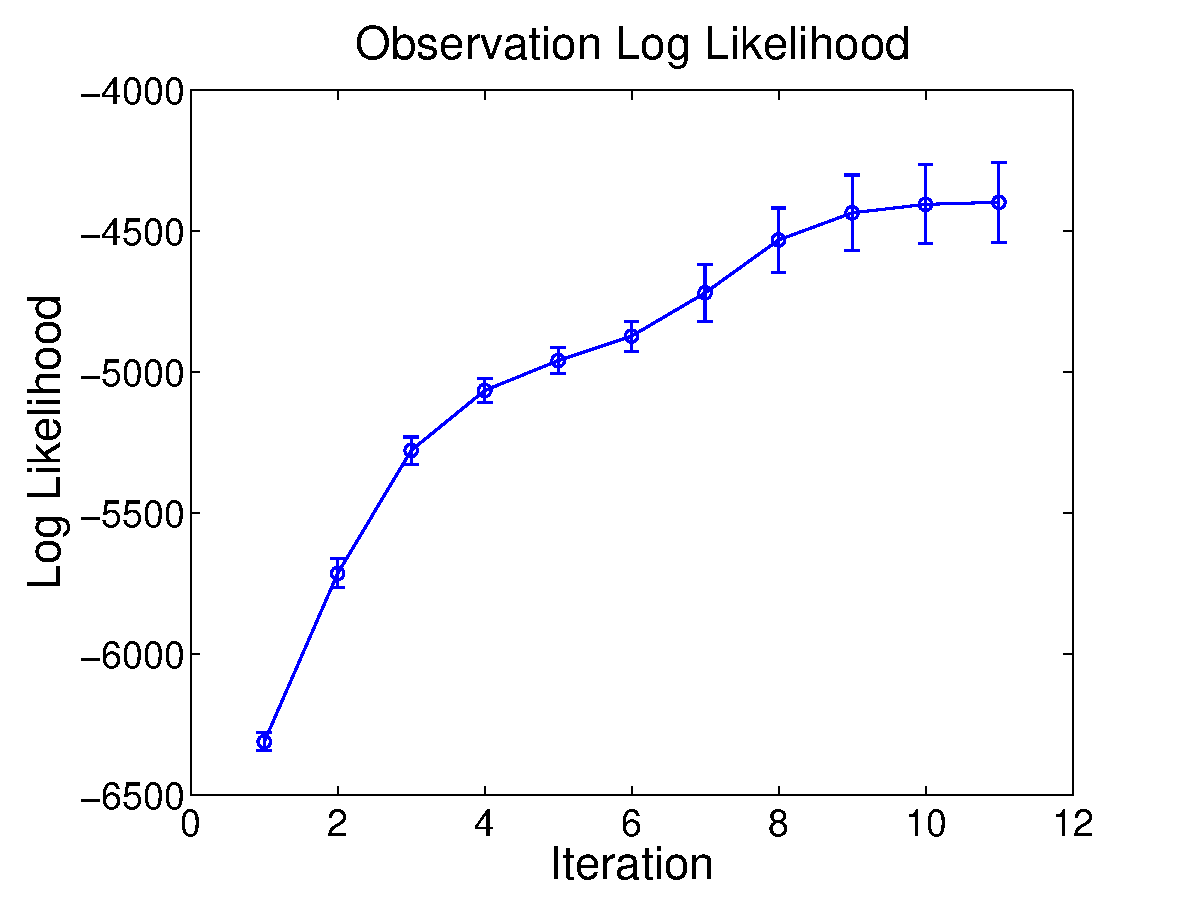
\includegraphics[width=1\textwidth]{crowd-thurstonian/figure/dp_loglikeli.eps}
      \caption{Log Likelihood} \label{fig::dp_loglikeli.eps}
		\end{subfigure}
	\caption{Domain Prediction Accuracy and Model Log Likelihood with Standard Deviations}
  \label{fig::dp}
\end{figure}

We use the setting of \textsc{Doc5Sr0.5Demo1} and generate the pairwise
preferences with only two domains evenly distributed among $100$ queries, for
the ease of illustration.  We run \textsc{Tpp} for $10$ times and plot the
prediction accuracy and the log likelihood. As shown in \Cref{fig::dp},
the algorithm starts from random guess with accuracy around $0.5$, and converges
to an accuracy around $0.895$ in less than $10$ iterations, implying that
\textsc{Tpp} is able to learn query domains effectively and efficiently.

\subsubsection{More Workers but Sparser Annotation}

In practice, when time is the constraining factor, it is plausible to employ a
large number of crowd workers and each worker labels only a few pairs. However,
the situation of \emph{``More Workers but Sparser Annotation''} can potentially
lead to a critical limitation for \tpp{}. On one hand, the number of
parameters $\{\tau_{k,m}\}$ grows with the number of workers. On the other hand,
the amount of data to estimate each $\tau_{k,m}$ decreases.

\begin{table}[h]
  \caption{\textsc{Tpp} Performance with More Workers but Sparser Annotation
  (Kendall's tau Distance)}
\begin{center}
\begin{tabular}{c|rl}
\hline \hline
Dataset	&	\multicolumn{2}{c}{Kendall's tau} \\ \hline \hline
\textsc{Anno100Sr0.01}	& $36.208$	& $\pm0.292$ \\
\textsc{Anno100Sr0.02} 	& $24.328$	& $\pm0.451$ \\
\textsc{Anno200Sr0.01} 	& $25.734$	& $\pm0.394$ \\
\textsc{Anno200Sr0.02} 	& $16.290$	& $\pm0.435$ \\ \hline \hline
\end{tabular}
\end{center}
\label{tab::sparse_anno}
\end{table}%


To evaluate the performance in such scenarios, we create another four datasets
under the setting of \textsc{Doc30Demo1} with more annotators (\textsc{Anno100}
of $100$ annotators and \textsc{Anno200} of $200$ annotators) and lower sparsity
ratios (\textsc{Sr0.01} and \textsc{Sr0.02}).

\begin{figure*}[t!]
    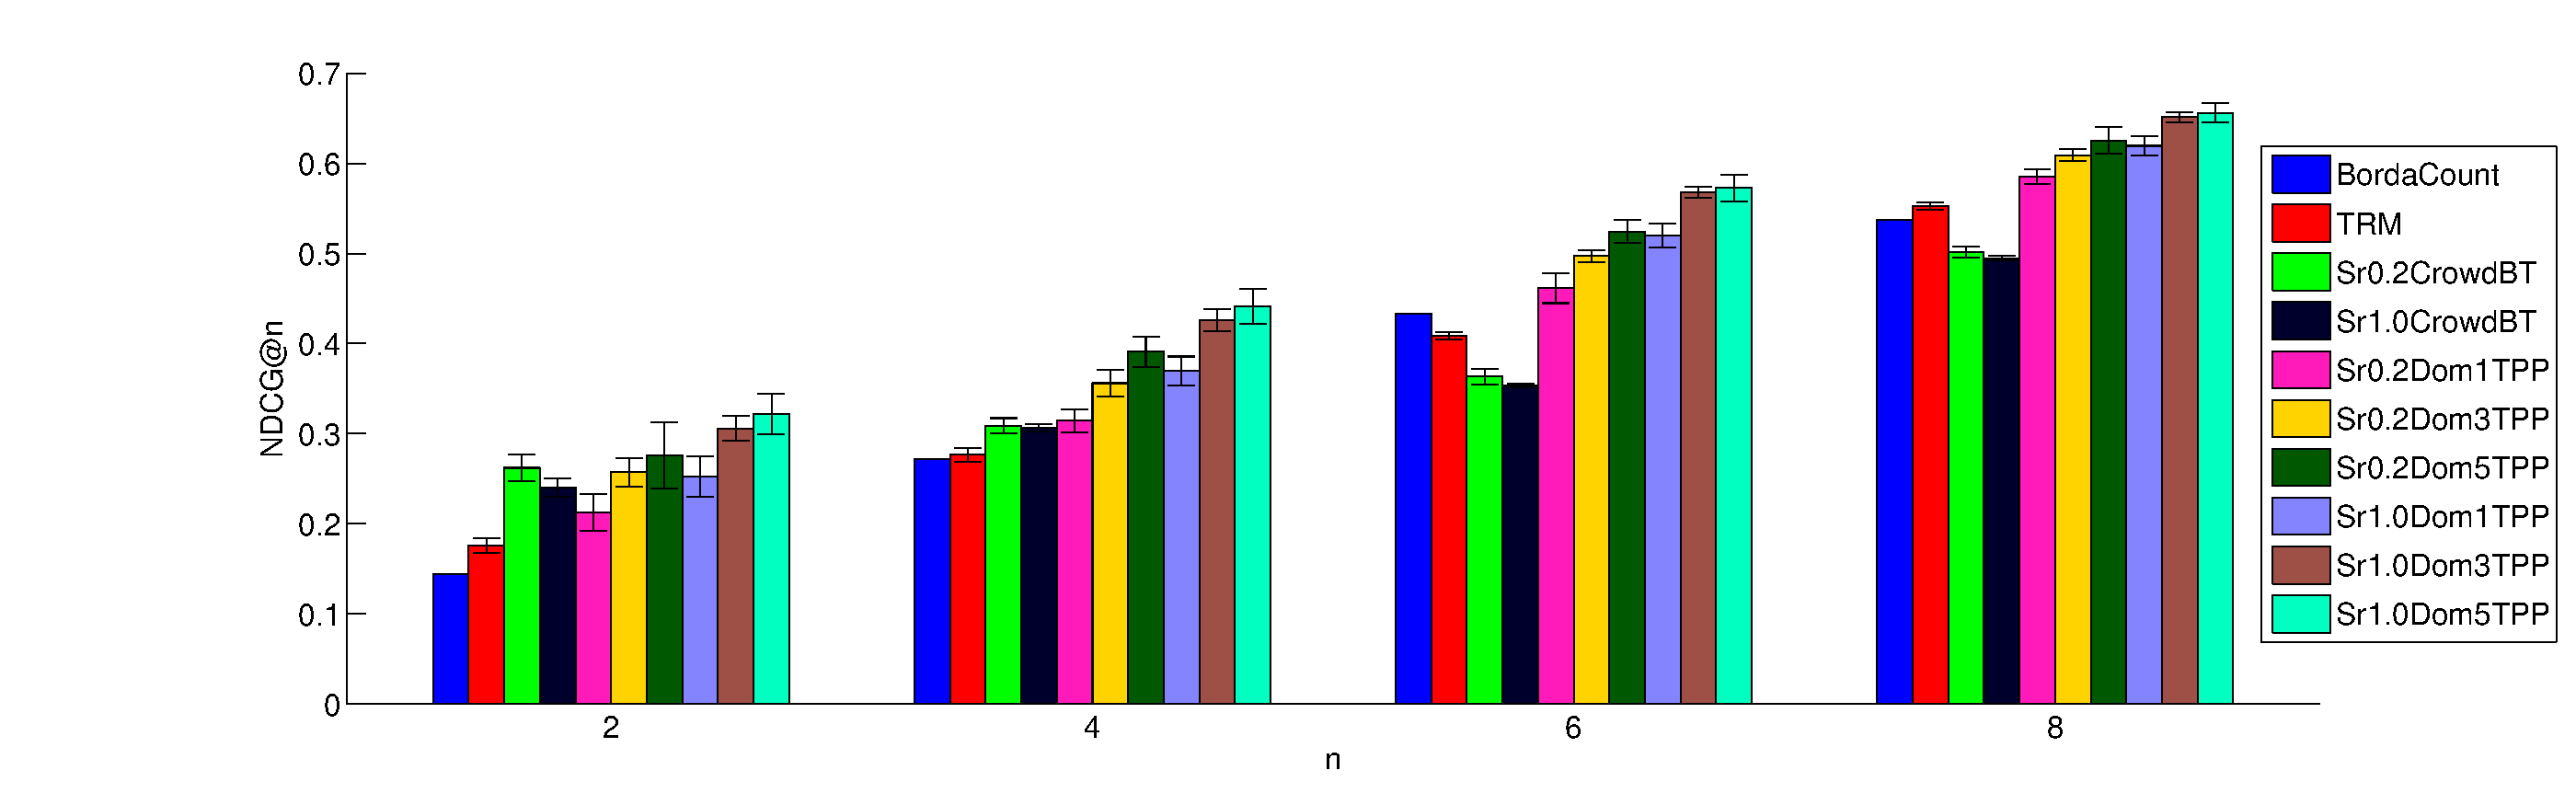
\includegraphics[scale= .4,trim={5cm 0 0 0},clip
      ]{crowd-thurstonian/figure/mq2008_agg.eps}
    \caption{NDCG@n evaluated on MQ2008-agg Dataset}
  \label{fig::mq2008_agg_jet}
\end{figure*}

As shown \Cref{tab::sparse_anno}, the performance of \textsc{Tpp} becomes
worse with ``More Workers but Sparser Annotation'' as Kendall's tau increases
from $22.442$ (\textsc{Doc30Sr0.1Demo1}) to $36.208$ (\textsc{Anno100Sr0.01}).
This is anticipated because the two datasets have the same amount of pairwise
judgements but \textsc{Anno100Sr0.01} involves more workers and has sparser
annotations.  However, \textsc{Anno100Sr0.01} drastically reduces the time cost
and may take only a tenth of the time that \textsc{Doc30Sr0.1Demo1} takes. In
fact, by doubling the number of workers to $200$ or doubling the sparsity ratio
to $0.02$, comparable performance can be achieved with \textsc{Doc30Sr0.1Demo1}.
With an even more aggressive setting \textsc{Anno200Sr0.02} ($20$ times the
number of workers and five times sparser annotations), the performance further
improves. Therefore we conclude that the performance of \tpp{} is reasonably
robust even at the situation of ``more workers and sparser annotation.''


\subsubsection{Malicious Worker Detection} Identifying malicious workers is a
difficult task since the number of malicious workers is usually small so that
the classification is highly imbalanced. We assess the performance of malicious
worker detection by plotting the averaged Receiver Operating Characteristic
(R.O.C.) curves in \Cref{fig::roc}.  In the experiment, with 100 workers
from \textsc{Demo1} and $\textsc{Sr} = 0.01$, \tpp{} performs well with
$\mathrm{AUC}=0.837$ (Area Under the Curve).  When the annotation is
denser~(\textsc{Anno100Sr0.02}),  AUC improves remarkably~($0.924$).  However,
with $200$ workers (\textsc{Demo1}), the difference of AUC between $\textsc{Sr =
0.01}$ and $\textsc{Sr = 0.02}$ is not significant. This can be explained by the
fact that malicious workers are easier to identify in a larger group, even with
sparser annotations.

\begin{figure}[h!]
  \begin{center}
    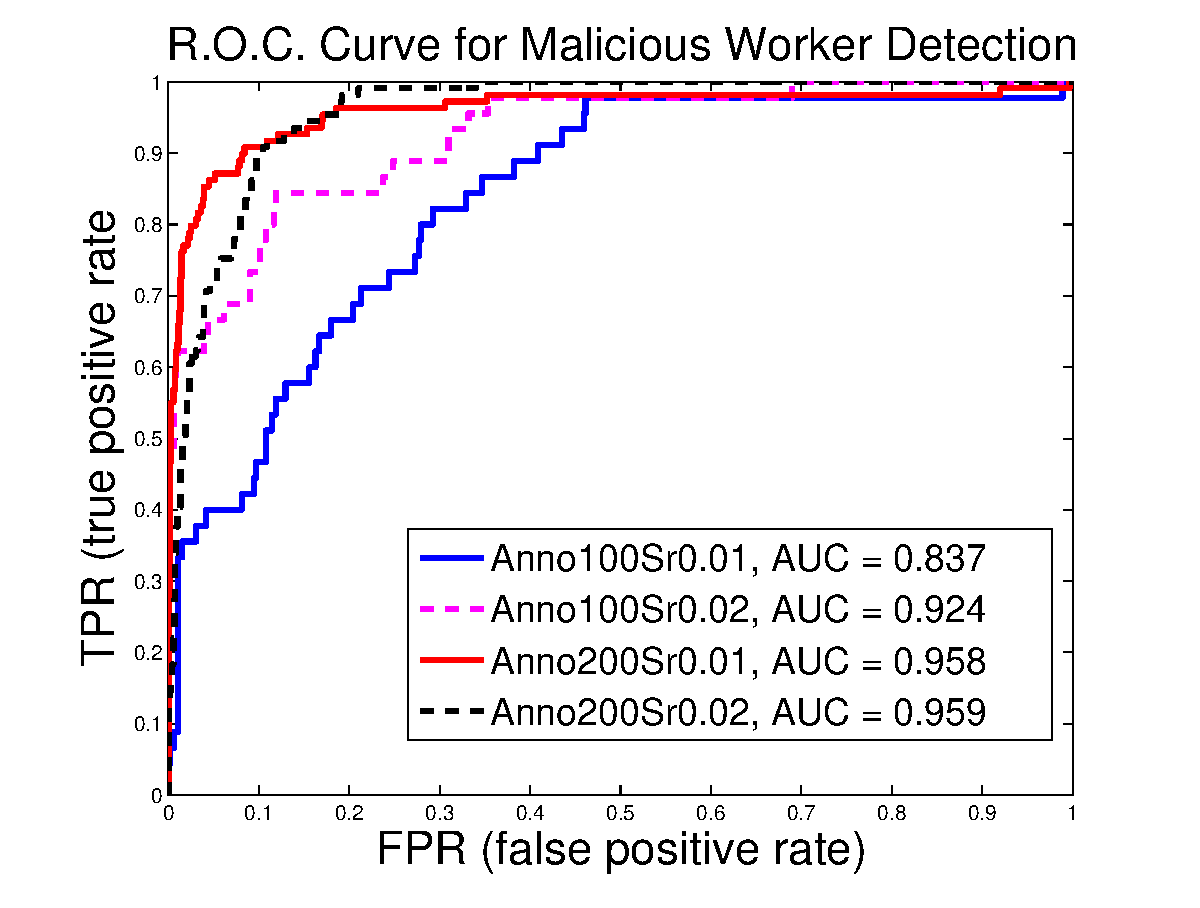
\includegraphics[scale= .50]{crowd-thurstonian/figure/roc.eps}
  \end{center}
  \caption{R.O.C. Curve for Malicious Worker Detection}\label{fig::roc}
\end{figure}

\subsection{Experiments on Real-World Data}

To validate our proposed strategy of binding pairwise preferences into rankings,
we utilize a real-world benchmark MQ2008-agg (part of LETOR
4.0\footnote{http://research.microsoft.com/en-us/um/beijing/projects/letor})
which is originally devised for the rank aggregation~(meta-ranking) task.  The
MQ2008-agg dataset consists of ranked lists from $25$ retrieval systems
(workers). Each document is labeled as \textit{highly relevant}~(2),
\textit{relevant}~(1) or \textit{irrelevant}~(0).  For rank aggregation
algorithms (\trm{} and BordaCount), ranked lists generated from each retrieval
system are taken as input to infer the true ranked list for each query. The
pairwise preference binding algorithms~(\textsc{Tpp} and \textsc{CrowdBt}), on
the other hand, estimate the true ranking out of the pairwise judgements from
each retrieval system (``worker''). The pairwise judgements are randomly sampled
with a sparsity ratio \textsc{Sr}.  In the experiment, we use sparsity ratios
$\textsc{Sr = 1.0}$ (all pairwise judgements are observed) and $\textsc{Sr =
0.2}$.  We evaluate \textsc{Tpp} with 1, 3 and 5 domains. The performance is
compared against both the pairwise preference binding algorithm
\textsc{CrowdBt}, and the rank aggregation algorithms
BordaCount~\cite{aslam2001models} and \textsc{Trm}~(see
\Cref{sec::tpp_trm} and \Cref{app::trm}). In particular,
Bordacount is a simple yet robust algorithm which is essentially a ranking
version of \emph{majority voting}. It infers the true ranking by averaging the
rank positions from each worker.  The performance is measured by NDCG
(Normalized Discounted Cumulative Gain) \cite{jarvelin2000ir}. We use NDCG@$n$
where $n = 2, 4, 6, 8$.

The results are presented in \Cref{fig::mq2008_agg_jet}. In general,
similar performances are observed for the two rank aggregation algorithms with
\textsc{Trm} slightly outperforming Bordacount. With \textsc{Sr1.0},
\textsc{Tpp} and \textsc{CrowdBt} have the same amount of information from
observations as the rank aggregation counterparts. However,
\textsc{Sr1.0CrowdBt} performs better than \textsc{Trm} and Bordacount only at
NDCG@2 and NDCG@4, while it gets worse at NDCG@6 and NDCG@8. In contrast, \tpp{}
consistently outperforms all the baselines, with better performance achieved if
more domains are incorporated.

When the available  annotations become sparser (\textsc{Sr0.2}), the performance
of both \textsc{Tpp} and \textsc{CrowdBt} become worse: NDCGs decrease across
different settings. However, \textsc{Tpp} still significantly outperforms
\textsc{CrowdBt} even with a single domain. In addition, it also outperforms
\textsc{Trm} and Bordacount although the annotation is incomplete. This is
because that the flexible generative process of \textsc{Tpp} properly resolves
the inconsistency from multiple sources.


\section{Related Work} \label{sec::tpp_related_work}

Early research of crowdsourcing can be dated back to the study of
\emph{integration of labels from multiple annotators} for image
classification~\cite{smyth1995inferring}. Later on, studies
including~\cite{yan2010modeling,whitehill2009whose} began focusing on explicitly
modeling annotator quality  such as expertise, truthfulness in crowdsourcing
settings. The dual tasks of inferring ground truth labels as well as worker
quality have been investigated in some recent
studies~\cite{yan2010modeling,whitehill2009whose,welinder2010multidimensional},
including this work.

Previous  research mainly focused on simple tasks (classification, regression,
etc.) while we tackle complex labeling problem such as ranking. In this
direction, \cite{steyvers2009wisdom} reconstructs the order of facts from
individual worker annotated \emph{whole ranked lists} with the Thurstonian
Ranking Model (\textsc{Trm})~\cite{thurstone1927law} and the Mallows
model~\cite{mallows1957non}, which features a distance-based distribution of
rankings~(permutations) using Kendall's tau.  Other studies on ``Rank
Aggregation'' are also related to this work, including
\cite{klementiev2008unsupervised,klementiev2009unsupervised}. They adapt the
Mallows model for inferring ground truth rankings as well as the quality of
ranking algorithms. However, the above approaches do not fit well for
information retrieval and web search tasks as it is not practical for annotators
to label the whole ranked lists. This motivates us to investigate binding
pairwise preferences from crowd workers into rankings.

There is one recent study~\cite{chen2013pairwise} that adopts a similar
philosophy, which extends the Bradley-Terry model, a pairwise special case of
the Plackett-Luce model~\cite{luce2005individual,plackett1975analysis}.
Nevertheless, their model (\textsc{CrowdBt}) lacks the mechanism to model
multiple query domains, thus incapable to characterize workers' domain-dependent
expertise and truthfulness. \textsc{CrowdBt} does not take query difficulty into
account either. Furthermore, unlike \textsc{Tpp}, \textsc{CrowdBt} does not
model the  generation of rankings. Therefore, it is not capable of modeling the
annotation inconsistency from multiple sources, which makes it less favorable as
demonstrated by the experimental study.

\section{Conclusions and Future Work} \label{sec::tpp_conclude}

In this chapter, we present a novel generative model called ``Thurstonian
Pairwise Preference'' (\textsc{Tpp}) to infer the true ranked list out of a
collection of crowdsourced pairwise annotations, which is highly useful in
various data mining and information retrieval tasks such as \emph{learning to
rank}. \tpp{} resolves the inevitable incompleteness and inconsistency of
pairwise judgements, by carefully modeling variable query difficulty and
different labeling quality resulting from workers' domain expertise and
truthfulness. Experimental results on both synthetic and real-world datasets
demonstrate that \textsc{Tpp} can effectively bind pairwise preferences of the
crowd into rankings and substantially outperforms previously published methods.
To further explore the benefit from the inferred ranked lists,  it is promising
to extend  \textsc{Tpp} to jointly learn the ranking model of the end
application, which we leave for future work.





\chapter{\DCME{} \\ with Application to Classification and Word
Embedding}\label{chp::dcme}
\section{Introduction}

We have already witnessed that PLVM is an excellent tool for modeling data of
different types. However, it is less explored whether we can leverage PLVM for
scalable and efficient optimization as well. In this chapter, a novel approach,
\DCME, is proposed to address the stability problem of Maximum Entropy when
there is an extreme large number of items (classes/words) present. The key
insight is that latent variables can be investigated to perform model reduction
and to facilitate inference. By incorporating the modeling of latent variables,
the dual space of the Maximum Entropy problem is explored and a K-means like
clustering is conducted over the simplex space. We demonstrate that leveraging
PLVM leads to an efficient algorithm, the complexity of which does not depend on
the number of items.

Maximum Entropy (ME), also known by a variety of other names, including
log-linear, Gibbs, exponential, softmax and multinomial logistic regression
models, is one of the most widely applied machine learning techniques in various
fields. As a classification method, ME has seen wide-scale applications in text
mining and natural language processing, such as text
classification~\cite{nigam1999using}, part-of-speech
tagging~\cite{ratnaparkhi1996maximum} and machine
translation~\cite{berger1996maximum}. In neural networks, ME (softmax) is the
building block of network architectures to transform a vector of signals into
probabilities~\cite{collobert2008unified}, and has been explored to learn neural
probabilistic language models~\cite{bengio2003neural}. In recent literature, a
number of word embedding algorithms have been proposed based on ME, including
skip-gram, continuous bag-of-words
(CBOW)~\cite{mikolov2013efficient,mikolov2013distributed} and log-bilinear
models~\cite{mnih2007three}, among others.

ME establishes a distribution of the exponential form over items (classes/words)
(\Cref{eq::me}\,). Scalability becomes a crucial challenge when the number of
items is large, which occurs nowadays in many real-world problems.  For example,
in a text classification problem of predicting the publishing venue for research
papers, the number of classes can easily exceed thousands on datasets such as
ACM digital library\footnote{\url{http://dl.acm.org/}}; for word embedding,
commonly used training corpora, with the English
Gigaword\footnote{\url{https://catalog.ldc.upenn.edu/LDC2011T07}} as an example,
typically have a vocabulary of hundreds of thousands, if not millions of words.

The main computational difficulty in ME comes from the fact that one has to
enumerate all items in order to obtain either the probability of a single item
or the corresponding gradient~\cite{mnih2012fast}. Consequently conventional ME
optimization techniques such as iterative
scaling~\cite{berger1996maximum,darroch1972generalized} and gradient-based
algorithms~\cite{tsuruoka2009stochastic,gao2007comparative} are very slow to
train with large numbers of items. In practice, sampling-based
methods~\cite{gutmann2010noise,mnih2012fast,bengio2008adaptive} are often
adopted since the complexity does not hinge on the number of items. However, one
drawback they possess is the inevitable sampling variance. Furthermore, only the
model parameters associated with the sampled items get updated at each training
instance, while the majority of the model is left unchanged, which leads to
inefficient learning.

To achieve learning efficiency with affordable computational cost, we propose a
\DCME{}~(DCME) approach. It optimizes ME in a primal-dual fashion, where the
multinomial \emph{dual distribution} for each instance is exploited. The key
step of DCME is to cluster the dual distributions and to approximate each of
them by the corresponding \emph{cluster center}. The dual clustering proceeds by
alternating between an online update of each instance's cluster assignment and
an offline calculation\footnote{In this chapter, the term ``offline'' is
equivalent to ``batch computation''. } of the cluster centers. This gives rise
to an efficient updating scheme which splits the computation of the model
subgradient into an \emph{online} part and an \emph{offline} part. Our proposed
DCME enjoys two desirable properties: (1) The model parameters associated with
\emph{all} items are updated at \emph{each} training instance, which ensures
learning efficiency; and (2) The computational cost per instance scales as the
product of the feature/word vector dimensionality\footnote{To be precise, by
taking advantage of sparsity, the complexity depends only on the number of
non-zero elements instead of the dimensionality of the vector.} and the number
of clusters, which yields fast training speed.

The rest of the chapter is organized as follows: \Cref{sec::dcme_review} reviews
the Maximum Entropy and existing approaches for learning with large numbers of
items. The proposed DCME is presented in \Cref{sec::dcme_dcme} with the
derivation and complexity analysis. The overall algorithmic procedure is
summarized in \Cref{sec::dcme_algo} where the theoretical advantages of DCME are
also discussed. Experimental studies on text classification and word embedding
are reported in \Cref{sec::dcme_experiments}, followed by conclusions in
\Cref{sec::dcme_conclusion}.

\section{Background} \label{sec::dcme_review}

\subsection{Maximum Entropy Framework}

The general formulation of ME is simple. For a data instance $t$, ME establishes
a distribution over $N$ items:

\begin{equation}
  \P_t(i; \THETA) = \frac{\exp(f_t(i; \THETA))}
  {\sum\limits_{j=1}^{N}\exp(f_t(j; \THETA))}, \quad  i = 1, \dots, N.
  \label{eq::me}
\end{equation}

where $f_t(i; \THETA)$ is the scoring function with model parameters $\THETA$,
which quantifies the affinity between instance $t$ and item $i$\footnote{In the
context of energy-based models, $-f_t(i; \THETA)$ is often referred as the
energy function~\cite{bengio2003neural}.}. In this chapter, we investigate ME in
two settings, namely, multi-class classification and word embedding.

For $N$-class classification, the dataset $\mathcal{D}$ consists of a collection
of instances $\{(\vx_t, i_t)\}$ with $\vx_t$ being a $D$-dimensional feature
vector and $i_t$ a label chosen from items $1, \dots ,N$.  The model $\vW =
[\vw_1, \dots, \vw_N]$ is a $D \times N$ matrix which specifies the scoring
function as:

\begin{flalign}
  & \cc && f_t(j; \THETA) = f_t(j; \vW) = \vw_j^T \vx_t &
  \label{eq::scr_classification}
\end{flalign}

In the word embedding setting, we focus our discussion on the continuous
bag-of-words algorithm (CBOW)~\cite{mikolov2013efficient}, but the analysis
easily extends to other models. As a language modeling technique, it predicts
the target word from a vocabulary of size $N$ given its surrounding context. The
$t$-th training instance contains a stream of words $w_{t,-c}, w_{t,-(c-1)},
\dots, w_{t,0}, \dots, w_{t, c-1}, w_{t,c}$ with the target word $i_t =
w_{t,0}$. CBOW calculates the compatibility between the $j$-th word in the
vocabulary and the context as:

\begin{flalign}
  &\ee
  && f_t(j; \THETA) = f_{t}(j; \vV, \vH) = f(\vv_j, \vhb_t) = \vv_j^T \vhb_t &
  \nonumber \\
  &&& \textrm{where}\quad \vhb_t = \frac{1}{2c}
  \sum\limits_{-c \le p \le c, p \neq 0} \vh_{w_{t,p}} &
  \label{eq::scr_embedding}
\end{flalign}

The model parameters $\vV=[\vv_1, \dots, \vv_N]$ and $\vH=[\vh_1, \dots,
\vh_N]$ are two $D \times N$ matrices of the ``input'' and ``output'' vector
representations of words, respectively.

\subsection{Optimization of ME}

Various algorithms for ME have been studied in the literature. They approach the
optimization by solving either the primal or the dual problem. The primal form
maximizes the log-likelihood of the dataset. Methods of this direction, as
surveyed in \cite{malouf2002comparison,yuan2012recent}, include iterative
scaling algorithms~\cite{berger1996maximum,darroch1972generalized}, coordinate
descent~\cite{huang2010iterative}, stochastic gradient
descent~\cite{tsuruoka2009stochastic} and Quasi-Newton
method~\cite{gao2007comparative}, just to name a few. Their training complexity
per instance is $\oo(DN)$. This is a consequence of having to enumerate
\emph{all} items when computing the probability of a single item or the
corresponding gradient. On the other hand, another line of research tackles the
problem by maximizing the entropy of \emph{dual distributions}.  Constraint
optimization techniques, such as exponentiated
gradient~\cite{collins2008exponentiated} and dual coordinate
descent~\cite{yu2011dual}, are investigated. Since the dimensionality of dual
distributions is in fact the same as the number of items, their training
complexity is still linear in $N$. Consequently, all these algorithms are
impractical with large numbers of items due to the prohibitively expensive
computational cost.

\subsection{Learning with Large Item Number}

Scaling algorithms for learning when the number of items $N$ is large have
become a recent research direction with focus on maintaining the training
complexity sublinear in $N$.  Among them, hierarchical approaches explore a
taxonomy (of items) and convert the problem into a series of binary predictions
along the tree branches, which potentially reduces the complexity from $\oo(N)$
to $\oo(\log N)$. Though efforts have been made in large multi-class (extreme)
classification~\cite{choromanska2015logarithmic,choromanska2013extreme} and word
embedding~\cite{morin2005hierarchical,mnih2009scalable,mikolov2013efficient},
finding balanced tree structures that provide an effective partition of items is
difficult by itself, and thus their use is limited in practice. Another work of
extreme classification, \cite{YenHRZD16}, has developed a fast active set
algorithm for max-margin classifiers by exploiting the sparsity of feature
vectors. The training speed-up, nevertheless, is generally insignificant for
dense data representations such as word embeddings. To the best of our
knowledge, the most effective approaches for training ME models with a large $N$
are sampling-based methods, for instance \cite{bengio2008adaptive}, offering a
trade-off between speed and precision. In addition, as pointed out by
\cite{mnih2012fast}, noise-contrastive estimation (NCE)~\cite{gutmann2010noise}
is regarded as the state-of-the-art sampling algorithm which employs the idea of
``learning by comparison'': It reduces the $N$-item ME problem to a binary
classification between samples from the training data and ``noise'' from the
proposal distribution, and is guaranteed to converge to the solution of ME. Yet
in practice, a slightly simpler variant, negative sampling
(NS)~\cite{mikolov2013distributed}, is proposed to train CBOW and skip-gram
though mathematically it does not solve ME. However, one drawback is that
algorithms of this kind inevitably suffer from sampling variance. More
crucially, the computational efficiency is gained at the expense of only
updating the model parameters associated with the sampled items, while the due
change of the rest is discarded. Learning efficiency is therefore sacrificed.

% In contrast, the proposed DCME can achieve much better learning efficiency while
% maintaining a computational cost comparable to these sampling-based methods.

\section{\DCME{}}\label{sec::dcme_dcme}

In this section, we present a \DCME{}~(DCME) approach which has two advantages
regarding learning and computational efficiency: (1) The model parameters
associated with \emph{all} items are updated at \emph{each} training instance;
and (2) The time complexity is independent of $N$.

\subsection{Primal-dual ME}

Different from existing approaches, DCME solves the ME problem in a primal-dual
fashion. Suppose that the dataset $\mathcal{D}$ has $M$ instances and $N$ items
where the $t$-th instance selects the $i_t$-th item. We start the derivation
from the primal ME formulation which maximizes the log-likelihood:

\begin{alignat}{-1}
  \sum\limits_{t=1}^M \log(\P_t(i_t; \THETA))=&
  \sum\limits_{t=1}^M \big(  f_t(i_t; \THETA)
  - \log \sum\limits_{j=1}^N \exp f_t(j; \THETA) \big) \nonumber\\
  =& \sum\limits_{t=1}^M \big(  f_t(i_t; \THETA) - A_t(\THETA) \big)
\label{eq::primal_ll}
\end{alignat}

where $A_t(\THETA)$ is referred to as the log-partition function and its
conjugate dual is revealed by the following
lemma~\cite{hiriart1993convex,wainwright2008graphical}:

\begin{lem}\label{lem::conj_dual}
  Assume $ \P(i; \vs) = \exp(s_i) / \sum\limits_{j=1}^N \exp(s_j)$
  and $A(\vs) = \log \sum\limits_{j = 1}^N \exp(s_j)$,
  the conjugate duality between the log-partition function and negative entropy
  states:

  \begin{align}
    A(\vs) &= \max\limits_{\vmu \in \Delta_N}
                    \{ \sum\limits_{j=1}^N \mu_j s_j -
                       \sum\limits_{j=1}^N \mu_j \log \mu_j \} \nonumber \\
           &= \max\limits_{\vmu \in \Delta_N}
                    \{ \E_{\vmu} [s_j] + \entropy(\vmu) \} \label{eq::conj_dual}
  \end{align}

  where the simplex set
  $\Delta_N = \{\mathbf{p} \in \mathbb{R}^{N}:
  p_j \ge 0, \sum\limits_{j=1}^N p_j = 1\}$

  and the maximizer is attained at:

  \begin{align}
    \mu_j^* = \P(j; \vs), \quad 1 \le j \le N \label{eq::conj_dual_sol}
  \end{align}

\end{lem}

\begin{proof}
  We use the following equivalence:
  \begin{align*}
    \E_{\vmu}[s_j] + \entropy(\vmu)
      &= -\sum\limits_{j=1}^N \mu_j \log \frac{\mu_j }{ \P(j; \vs) } +
          \log\sum\limits_{j=1}^N \exp(s_j) \nonumber \\
      &= -D_{KL}(\vmu || \P) + A(\vs)
  \end{align*}
where $D_{KL}(\vmu || \P)$ is the Kullback-Leibler (KL) divergence and note
$D_{KL}(\vmu || P) \ge 0$ and  $D_{KL}(P || P) = 0$. It follows that
$\vmu^* = \argmin\limits_{\vmu \in \Delta_N} D_{KL}(\vmu || P) = P$.
\end{proof}

In view of \Cref{lem::conj_dual}, we arrive at the primal-dual form of ME:

\begin{equation}
  \max\limits_\THETA
  \min\limits_{\substack{\vmu_t \in \Delta_N \\ 1 \le t \le M}}
  \sum\limits_{t=1}^M \big( f_t(i_t; \THETA) - \E_{\vmu_t}[f_t(j;\THETA)] -
  \entropy(\vmu_t) \big) \label{eq::me_primal_dual}
\end{equation}

where $\vmu_t$ is the \emph{dual distribution} for instance $t$.

\subsection{Dual Distribution Clustering}

\Cref{lem::conj_dual} implies that $\vmu_t^*$ is determined by $f_t(j;\THETA)$.
In less mathematical terms, similar instances choose similar items (in
probabilities). As real-world data instances generally possess a clustering
structure instead of being randomly distributed, it is expected that dual
distributions also form clusters. For the text classification example of venue
prediction, if papers are grouped by topics, those in the same group should have
similar chance of getting published at a particular venue; For learning word
embedding, we anticipate contexts of similar semantics yield target word
distributions that can be clustered together.

It is worth exploring the cluster structure of dual distributions to reduce
complexity. DCME rests on the idea of ``approximation by clustering'': By
clustering the dual distributions into $K$ groups, each $\vmu_t$ is assigned to
a cluster $c_t \in \{1, \dots K\}$, and is then approximated by the
corresponding \emph{cluster center} $\valpha_{c_t}\in\Delta_N$ which best
represents the group. The optimization problem of DCME can thus be formulated
as:

\begin{alignat}{-1}
  &\textrm{DCME:} && \qquad
\max\limits_\THETA
\min\limits_{\substack{\valpha_k \in \Delta_N \\ 1 \le k \le K}}
\min\limits_{\substack{1 \le c_t \le K \\ 1 \le t \le M}}
\sum\limits_{t=1}^M Q_t(\valpha_{c_t}; \THETA) \label{eq::dcme} \\
  &\textrm{where~~} &&
Q_t(\valpha_{c_t}; \THETA) =
  f_t(i_t;\THETA) -
  \E_{\valpha_{c_t}}[f_t(j;\THETA)] -
  \entropy(\valpha_{c_t})\big) \nonumber
\end{alignat}

\subsection{Online-Offline Optimization}

We employ Gauss-Seidel coordinate descent to solve \Cref{eq::dcme}.  Three
blocks of variables, namely, the model parameters $\THETA$, the cluster centers
$\{\valpha_k\}$, and the instances' cluster assignments $\{c_t\}$, are
successively updated while keeping others constant. In particular, we devise a
hybrid online-offline algorithm which breaks the computational bottleneck and
leads to a time complexity that only scales as $\oo(DK)$, as opposed to
$\oo(DN)$ in conventional ME algorithms.

\subsubsection{Updating cluster assignments~(Online)}

DCME approximates $\vmu_t$ by $\valpha_{c_t}$, and the cluster assignment $c_t$
is solved by:

\begin{equation}
  \argmin\limits_{1 \le k \le K} - \E_{\valpha_{k}}[f_t(j;\THETA)]
        - \entropy(\valpha_{k}) \label{eq::clu_mem}
\end{equation}

However, a na\"{i}ve computation would cost $\oo(DN + KN)$ time. It takes
$\oo(D)$ to evaluate $f_t(j;\THETA)$ for every item $1 \le j \le N$\footnote{In
  word embedding, one can compute the scoring function in $\oo(D)$ time. Note
  that the \emph{asymptotic} complexity of computing $\vhb_t$ in \emph{every}
sliding windows is $\oo(D)$ (independent of window size) with the sum $\sum_{-c
\le p \le c} \vh_{w_{t,p}}$ maintained by adding the new word and subtracting
the past word.}; For each cluster, another $\oo(N)$ is required to calculate
$\E_{\valpha_{k}}[f_t(j;\THETA)]$ and $\entropy(\valpha_k)$ by enumeration.

Fortunately, when the scoring function is linear in the feature/context vector,
the cost can be reduced to $\oo(DK)$ per instance. To see this, from
\eqref{eq::scr_classification} and \eqref{eq::scr_embedding} we have:

\begin{alignat}{-1}
  &\cc &
  \E_{\valpha_{k}}[f_t(j; \vW)] &= (\vW \valpha_{k})^T \vx_t
  \label{eq::exp_classification}\\
  &\ee &
  \E_{\valpha_{k}}[f_t(j; \vV,\vH)] &= (\vV \valpha_{k})^T \vhb_t
  \label{eq::exp_embedding}
\end{alignat}

The trick we apply here \emph{trades memory for time}: By storing $\vW
\valpha_{k}$, $\vV \valpha_{k}$ and $\entropy(\valpha_k)$ for $K$ clusters in
the offline update, it is merely a $D$-dimensional dot product to calculate
\Cref{eq::exp_classification} and \Cref{eq::exp_embedding}, and therefore the
cost to online update $c_t$ by \Cref{eq::clu_mem} is $\oo(DK)$.

\subsubsection{Updating cluster centers~(Offline)}

We update the cluster center $\valpha_k$ as well as the cached $\vW
\valpha_{k}$, $\vV \valpha_{k}$ and $\entropy(\valpha_k)$ only in the offline
computation. Let $\ii_k$ denote the index set of instances in the $k$-th
cluster, $\valpha_k$ satisfies:

\begin{align}
   \argmin\limits_{\valpha \in \Delta_N}
   -\E_{\valpha}\Bigg[\frac{1}{|\ii_k|}
                      \sum\limits_{t \in \ii_k}f_t(j; \THETA)\Bigg]
   -\entropy(\valpha) \label{eq::up_clu_center_opt}
\end{align}

Invoking \Cref{lem::conj_dual} again, \Cref{eq::up_clu_center_opt} has the
following closed-form solution:

\begin{align}
  \alpha_{k, j} = \frac{1}{Z} \exp\big(
      \frac{1}{| \ii_k |}
      \sum\limits_{t \in \ii_k} f_t(j;\THETA) \big)
  \label{eq::up_clu_center}
\end{align}

where a normalization term $Z$ is applied to keep $\sum\limits_{j=1}^N
\alpha_{k,j} = 1$. By the linearity of $f_t(j;\THETA)$, we express
\Cref{eq::up_clu_center} as:

\begin{alignat}{-1}
  &\cc & \quad
  \alpha_{k, j} = \frac{1}{Z} \exp\Big( \vw_j^T
  \frac{1}{| \ii_k |} \sum\limits_{t \in \ii_k} \vx_t\Big)
  \label{eq::up_clu_center_classification}\\
  &\ee &
  \alpha_{k, j} = \frac{1}{Z} \exp\Big( \vv_j^T
  \frac{1}{| \ii_k |} \sum\limits_{t \in \ii_k} \vhb_t\Big)
  \label{eq::up_clu_center_embedding}
\end{alignat}

which computes $\valpha_k$ with $\oo(D |\ii_k|  + D N)$ cost. In addition, it
takes $\oo(DN)$ and $\oo(N)$ to update $\vW \valpha_{k}$, $\vV \valpha_{k}$ and
$\entropy(\valpha_k)$, respectively. By choosing the interval between
consecutive offline updates such that $|\ii_k| = \beta N$ for a constant $\beta$
(1 for example), we obtain an average time complexity of $\oo(D)$ per instance.

\subsubsection{Updating model parameters~(Online/Offline)}

To optimize $\THETA$ with subgradient descent:

\begin{alignat}{-1}
  &\cc &
  \frac{\partial Q_t}{\partial \vw_j} &=
    \underbrace{\mathds{1}[i_t = j]\, \vx_t}_{(a)} +
    \underbrace{(-\alpha_{c_t, j} \vx_t)}_{(b)}
    \label{eq::mdl_upd_classification}\\
  &\ee &
  \frac{\partial Q_t}{\partial \vv_j} &=
    \overbrace{\mathds{1}[i_t = j]\, \vhb_t} +
    \overbrace{(-\alpha_{c_t, j} \vhb_t)}
    \label{eq::mdl_upd_embedding_v}\\
  &&
  \frac{\partial Q_t}{\partial \vh_{w_p^{(t)}}} &=
    \frac{1}{2c} (\vv_{i_t} - \vV \valpha_{c_t})
    \label{eq::mdl_upd_embedding_h}\\
  &&
  \textrm{for all}\; &-c \le p \le c,\; p \ne 0 \nonumber
\end{alignat}

where $\mathds{1}[i_t = j]$ is the indicator function which evaluates to 1 when
$i_t = j$ and 0 otherwise. In the following, we devise a hybrid
\emph{online-offline algorithm} which has an average expense of $\oo(D)$ time
per instance.

First, Term (a) in \Cref{eq::mdl_upd_classification} and
\Cref{eq::mdl_upd_embedding_v} only changes the model parameters associated with
the correct item $i_t$, namely $\vw_{i_t}$ and $\vv_{i_t}$, and can be updated
online in $\oo(D)$ time. Similarly, for word embedding
\Cref{eq::mdl_upd_embedding_h}, $\partial Q_t / \partial \vH$ can also be
updated online with $\oo(D)$ cost by keeping track of the sum of $\partial Q_t /
\partial \vh_{w}$ for all overlapping instances using a sliding window
technique.

Second, Term (b) in \Cref{eq::mdl_upd_classification} and
\Cref{eq::mdl_upd_embedding_v} changes the model parameters of all $N$ items.
We make two crucial observations here: (1) Term (b) of different items share the
\emph{same} direction $-\vx_t$ (or $-\vhb_t$); and (2) The scale vector
$\valpha_{c_t}$ \emph{only} depends on the cluster assignment $c_t$, but not the
individual instance $t$. Thus it is logical to perform offline update of Term
(b). The computation is postponed until $|\ii_{c_t}|$ is large enough, and then
Term (b) is calculated for all items $1 \le j \le N$ and instances $t \in
\ii_{c_t}$. Such ``lazy'' computation yields a total cost of $\oo(D |\ii_{c_t}|
+ D N)$, and we achieve an average $\oo(D)$ expense per instance if we wait
until $|\ii_{c_t}| \ge \beta N$.

\subsubsection{Tuning online/offline computation}

The overall complexity per instance is $\oo(DK)$ time, which is appealing as it
does not hinge on $N$.  Nevertheless, an inherent limitation in learning is the
delay of computing Term (b) until $|\ii_k| \ge \beta N$ in
\Cref{eq::mdl_upd_classification} and \Cref{eq::mdl_upd_embedding_v} ,
especially for items with large values $\alpha_{k, j}$. A heuristic improvement
we find effective in practice tunes the computation between online and offline
updates. By sorting items (using a heap) with decreasing $\alpha_{k,j}$, Term
(b) of the top $Q$ items are updated online while the others are updated
offline. The resulting average cost per instance becomes $\oo(D K + D Q + \log
Q)$. Computational efficiency is preferred with a small $Q$ while the priority
shifts to learning efficiency with a large $Q$.

\section{DCME Algorithm}\label{sec::dcme_algo}

We have already presented the DCME algorithm in previous section. In the
following, we first give an overview about the DCME algorithm, and then
illustrate its connections with K-means algorithm and the Dual ME respectively.

\subsection{Overall Procedures}

We summarize the learning procedure of DCME in \Cref{alg::dcme}. DCME assigns
each training instance $t$ to a dual cluster $c_t$ and performs the online model
update. Once the size of a dual cluster reaches $\beta N$, an offline model
update as well as the update of the dual cluster center are applied.  Although
the algorithm has a similar complexity as the sampling-based approaches such as
noise contrastive estimation~(NCE) and negative sampling~(NS), DCME allows the
\emph{entire} model to learn from \emph{every} training instance. In other
words, the model parameters associated with all items get updated when a new
training instance arrives, which yields superior performance over existing
methods, as will be shown in the experimental study.

\begin{algorithm}[h]
\caption{DCME algorithm}\label{alg::dcme}
  % \SetAlgoNoLine
  \KwIn{$M$ instances, a constant $\beta$, cluster number $K$, and top item
        number $Q$}
	\KwOut{Model $\mathbf{\THETA}$}
  Initialize $K$ clusters $\{\valpha_k\}$ \;
	\While{$\THETA$ is not optimal}{
    \begin{itemize}
      \item[--] Select an index $t$ from $\{1, \dots, M\}$
      \item[--] Find the cluster assignment $c_t$ by \eqref{eq::clu_mem}
      \item[--] Perform online update of Term (a) (and Term (b) of the \\
                 top $Q$ items) in \eqref{eq::mdl_upd_classification} (or
                \eqref{eq::mdl_upd_embedding_v}). For embedding, also \\
                update $H$ by \eqref{eq::mdl_upd_embedding_h}.
      \item[--] Add $t$ to $\ii_{c_t}$; \\
                if $|\ii_{c_t}| \ge \beta N$
        \begin{itemize}
          \item[--] Perform offline update of Term (b) in
                    \eqref{eq::mdl_upd_classification} (or
                    \eqref{eq::mdl_upd_embedding_v}).
          \item[--] Update cluster center $\alpha_{c_t}$ and empty
                    $\ii_{c_t}$
        \end{itemize}
    \end{itemize}
	}
\end{algorithm}

\subsection{Connection with K-means}

So far, readers might have already been aware of the resemblance between the
dual distribution clustering and the K-means algorithm. The following theorem
formally proves their connection:

\begin{thm}
  The dual distribution clustering in DCME is a generalized K-means
  algorithm using KL-divergence as the distance measurement in the simplex.
  Moreover, it converges as fast as K-means.
\end{thm}
\begin{proof}
  Using \Cref{lem::conj_dual}, the dual clustering satisfies:

  \begin{alignat}{-1}
    \min\limits_{\substack{\valpha_k\in \Delta_N ,  1 \le k \le K \\
                           1 \le c_t \le K , 1 \le t \le M}} \;
  \sum\limits_{t=1}^M D_{KL}(\valpha_{c_t} || P_t) \label{eq::k-means_clustering}
  \end{alignat}

  which minimizes the \emph{within-cluster KL-divergence} between
  $\valpha_{c_t}$ and $P_t$. It is the same minimization objective as K-means
  except that DCME measures the distance in the simplex space with
  KL-divergence\footnote{Technically, KL-divergence is not a true metric of
  distance.}. To illustrate this, notice that the dual clustering proceeds by
  alternating between the following two steps (See \Cref{fig::dual_cluster}):

\begin{itemize}
\item[--] Update $c_t = \argmin_{k} D_{KL}(\valpha_k || P_t)$, and $t$ is
  assigned to the cluster whose center is nearest to $P_t$ by KL-divergence.
\item[--] Update $\valpha_k = \argmin_{\valpha} \sum_{t \in \ii_k} D_{KL}(
  \valpha || P_t)$ where the cluster center is found as the point in the simplex
  with the least within-cluster distance.
\end{itemize}

General convergence results for the subgradient methods can be applied.
Specifically, the above two-step algorithm converges to the local minimum of the
problem \eqref{eq::k-means_clustering} as fast as the K-means
algorithm~\cite{bottou1995convergence},
\end{proof}

\begin{figure}[h!]
  \centering
  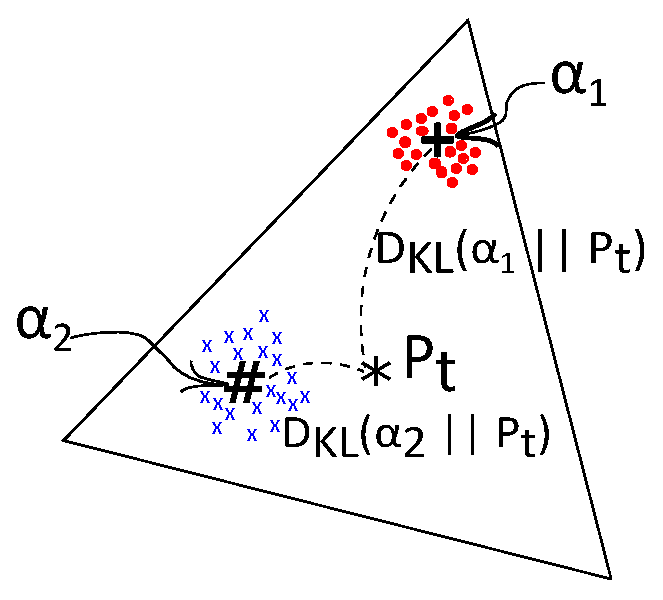
\includegraphics[width=0.4\linewidth]{dcme/dual_cluster_color.eps}
  \caption{Dual Clustering in the Simplex with KL-divergence}
  \label{fig::dual_cluster}
\end{figure}

\subsection{Connection with Dual ME}

The DCME is reminiscent of the dual ME, and we show the following results in the
classification setting:

\begin{thm} The dual form of DCME in classification is:
  \begin{align}
    \max\limits_{\substack{\valpha_k \in \Delta_N ,  1 \le k \le K \\
                           1 \le c_t \le K , 1 \le t \le M}}
                 &\qquad
    \sum\limits_{t=1}^M \entropy(\valpha_{c_t}) \label{eq::dual_dcme_op} \\
    \subjto \quad
    & \sum\limits_{t = 1}^M \mathds{1}[i_t = j]\; \vx_t =
    \sum\limits_{t = 1}^M \alpha_{c_t, j} \vx_t,~~ 1 \le j \le N \nonumber
  \end{align}
\end{thm}

The proof is omitted because it is very similar to the derivation of dual ME.
However, the dual form of DCME provides us with intuition of how DCME works: To
approximate $P_t$, the cluster center is restricted to reproduce the observed
statistics. Comparing it with the dual ME where $\vmu_t$ is in place of
$\valpha_{c_t}$, we see that the dual DCME has more restricted constraints. A
limiting case that DCME becomes identical to ME is when $K=M$, \ie{} each
instance is a singleton cluster with the only member being itself.

\section{Experiments}\label{sec::dcme_experiments}

We conduct experiments on tasks of text classification and word embedding,
evaluating the proposed DCME approach by examining its computational and
learning efficiency. For comparison, we implement two sampling-based approaches,
noise contrastive estimation~(NCE) and negative sampling~(NS), as well as the
maximum likelihood estimation using gradient descent~(GD). In order for DCME and
the sampling-based approaches to have comparable training speed, we set both the
cluster number $K$ of DCME and the sampling number of NCE and NS to 20, and also
control the interval between offline updates in DCME with $\beta = 1$. Two
variants of DCME, DCME-Q0 and DCME-Q10, are developed, the latter of which
applies the online/offline tuning with $Q=10$. All the algorithms are run with
20 threads in parallel on a 64-bit Linux machine with the Intel Xeon 3.60GHz CPU
(20 core). Our code is implemented in C and available for download at:
\url{https://www.dropbox.com/s/e6b3fj2w0lq6jbt/code.tar.gz}

\begin{figure*}
  \centering
        \begin{subfigure}[h]{0.7\textwidth}
            \centering
            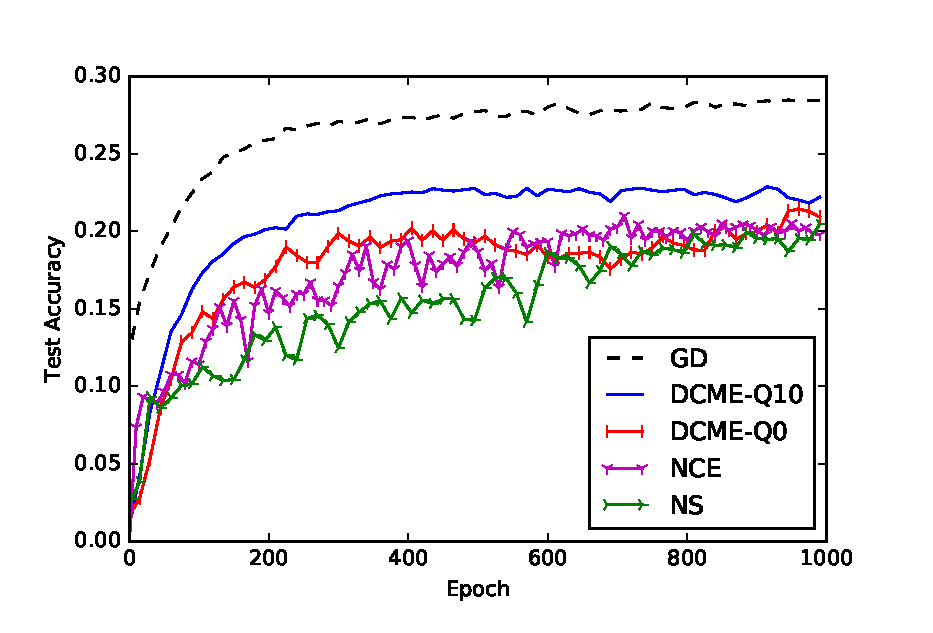
\includegraphics[width=\linewidth]{dcme/classification.eps}
            \captionsetup{justification=centering}
            \caption{Comparison of Test Accuracy for Classification\\
              Trained on ACM Digital Library Dataset}
            \label{fig::classification}
        \end{subfigure}
        \hfill
        \begin{subfigure}[h]{0.7\textwidth}
            \centering
            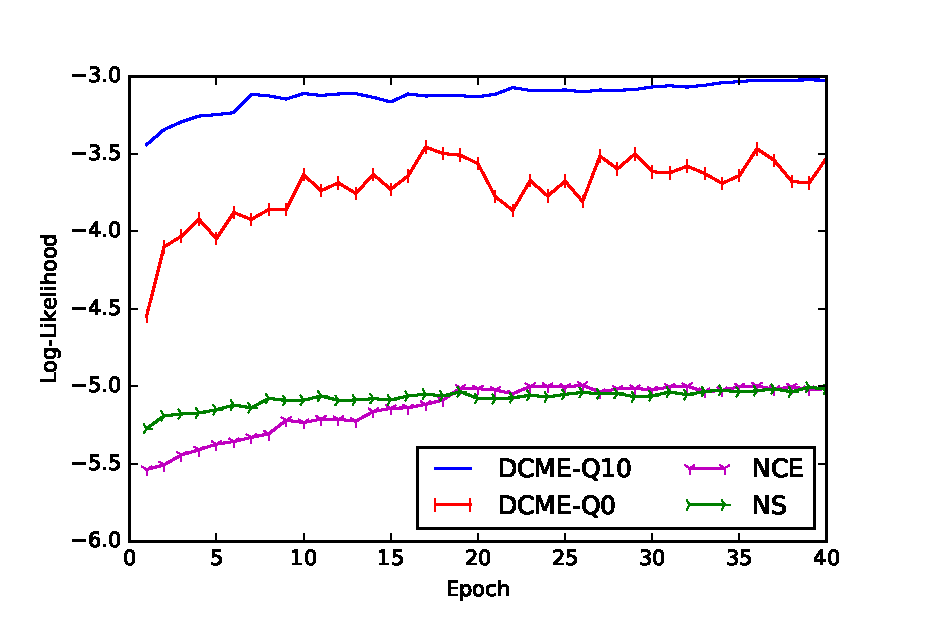
\includegraphics[width=\linewidth]{dcme/word_embedding.eps}
            \captionsetup{justification=centering}
            \caption{Comparison of Log-Likelihood for Embedding \\
              Trained on NYT Dataset}
            \label{fig::word_embedding}
        \end{subfigure}
        \begin{subfigure}[h]{0.65\textwidth}
            \centering
            \begin{tabular}{c|c|c|c|c}
              DCME-Q10  & DCME-Q0   & NCE   & NS        & GD     \\ \hline\hline
              9.50      & 7.94      & 6.21  & 6.16      & 165.91 \\
            \end{tabular}
            \captionsetup{justification=centering}
            \caption{Time Cost (Second) per Epoch in Classification}
            \label{tab::classification_time}
        \end{subfigure}
        \begin{subfigure}[h]{0.65\textwidth}
            \centering
            \begin{tabular}{c|c|c|c}
              DCME-Q10  & DCME-Q0   & NCE     & NS       \\ \hline\hline
              33.49     & 25.59     & 22.22   & 20.80    \\
            \end{tabular}
            \captionsetup{justification=centering}
            \caption{Time Cost (Minute) per Epoch in Embedding}
            \label{tab::we_time}
        \end{subfigure}
        \caption{ Performance on Text Classification and Word Embedding }
\end{figure*}

\subsection{Evaluation on Text Classification}

We employ the ME model to predict the publishing venue of research papers using
the abstract. A public dataset ACM Digital Library is investigated. It has
$162,460$ papers published at $1,236$ conferences. We hold out $10\%$ of the
documents for testing. Each paper is represented by the word count features of
the top $30,000$ frequent words.

\Cref{fig::classification} shows the learning curves of algorithms trained
at each epoch, and \Cref{tab::classification_time} reports the training
speed. It is clear that GD does not scale well to large number (thousands or
more) of items. DCME is 17-20 times faster than GD while the ratio is around 26
for sampling-based approaches. But it does give an estimation about the
upper-bound performance by leveraging the exact gradient information.  The curve
of GD converges in the least number of iterations while the test accuracy is the
highest.

DCME, on the other hand, achieves a computational efficiency similar to that of
the sampling-based approaches, but the accuracy is considerably higher.
Particularly, \Cref{fig::classification} validates that DCME benefits from
tuning the computation between online and offline updates. When $Q=10$, more
model parameters are updated online and there is thus less delay than that of
DCME-Q0. We also note that NCE and NS produce larger variances, which is
expected due to their sampling nature.

\subsection{Evaluation on Word Embedding}

For the word embedding task, we explore the New York Times (NYT) corpus from the
English Gigaword (Fifth Edition). It has a total of 1.35 billion words with
10.84 million unique terms. We retain the top 1 million frequent terms in the
vocabulary. To assess the performance, a randomly sampled \SI{1e-4} of the text
is withheld for testing. We train the word embeddings using CBOW with a context
window size of 10 and embedding dimensionality of 100.

We plot the test set average log-likelihood of each epoch in
\Cref{fig::word_embedding}, and report the time-per-epoch statistics in
\Cref{tab::we_time}. We do not evaluate GD in word embedding as it takes more
than days to run one epoch. The time costs for other algorithms are similar. The
results show that DCME remarkably outperforms NCE and NS.  However, DCME-Q0
exhibits a large performance variance. One possible explanation is as follows.
For $N$ as large as 1 million, the interval between offline updates is so long
that it creates two undesirable effects: (1) The delay results in a biased model
which contributes to a large training error; (2) The offline computation changes
the model drastically, as measured by the norm of the model difference, causing
inconsistency when another thread accesses the model while the offline update is
still in progress\footnote{The model parameters are shared by all threads and
  there is no mutex locks on writing to the model, which is a common practice
for efficiency in implementations including word2vec
  (\url{https://code.google.com/p/word2vec/}) and ours.}. For DCME-Q10, minimal
  variance is observed. Indeed, it offers the best trade-off between learning
  and computational efficiency.

\begin{table}[h]
  \centering
  \begin{tabular}{c||l|l|l}
    Model     & Semantic          & Syntactic         & Overall          \\
    \hline\hline
    DCME-Q10  & $\mathbf{-8.676}$ & $-8.648$          & $\mathbf{-8.654}$ \\
    DCME-Q0   & $-8.712$          & $\mathbf{-8.647}$ & $-8.663$          \\
    NCE       & $-8.784$          & $-8.782$          & $-8.783$          \\
    NS        & $-8.765$          & $-8.679$          & $-8.699$          \\
  \end{tabular}
  \captionsetup{justification=centering}
  \caption{Log-Likelihood on Semantic-Syntactic Word Relationship Dataset}
  \label{tab::we_analogy}
\end{table}

To assess the quality of the trained embeddings, we use the word analogy task,
which examines whether the embeddings learn the semantic/syntactic relationships
of words. For instance, the question which word is similar to ``small'' in the
same sense as ``biggest'' to ``big'' can be solved by predicting the target word
with a context vector $\vh_{biggest} - \vh_{big} + \vh_{small}$. We evaluate the
trained word embeddings after 15 epochs. And the results on the
Semantic-Syntactic Word Relationship test set~\cite{mikolov2013efficient} are
summarized in \Cref{tab::we_analogy}, where the best performance is highlighted
in bold. Again, it confirms that DCME achieves better model quality than
sampling-based NCE and NS.

% since they represent the main state of the art methods that can work efficiently with large numbers of items for ME.

% 0.017287 %   Semantic accuracy: 0.016449 %   Syntactic accuracy: 0.017556 %
% 0.017426 %   Semantic accuracy: 0.017061 %   Syntactic accuracy: 0.017543 %
% 0.016231 %   Semantic accuracy: 0.015777 %   Syntactic accuracy: 0.016377 %
% w2v
% 0.016666 %   Semantic accuracy: 0.015606 %   Syntactic accuracy: 0.017006 %
% 0.015336 %   Semantic accuracy: 0.015305 %   Syntactic accuracy: 0.015346 %
% 0.015792 %   Semantic accuracy: 0.015731 %   Syntactic accuracy: 0.015811 %

\section{Conclusions}\label{sec::dcme_conclusion}

We propose a novel optimization method, \DCME{}~(DCME), which solves the Maximum
Entropy problem in its primal-dual form. Although it has a similar complexity as
the sampling-based approaches, it allows the entire model to learn from every
training instance, which we believe is the first algorithm that is efficient
both in learning and computation. DCME exploits the dual clustering and
approximates dual distributions by cluster centers. It maintains an affordable
complexity using a hybrid online-offline optimization algorithm. Empirical
studies demonstrate that DCME outperforms state-of-the-art algorithms such as
NCE and NS in learning tasks with large numbers of items. A promising future
research direction is to investigate the nonparametric mixture models for dual
clustering. By taking advantages of probabilistic latent cluster assignments and
learning the number of clusters from the data, we expect a better approximation
for dual distributions.


\chapter{PLANS: \PLANS{}}\label{chp::plans}
\section{Introduction}

Learning distributed representations (embeddings) of language has been a very
attractive topic in recent development of natural language processing. Word
embedding assigns a (usually dense) low dimensional vector to each word which is
supposed to retain the semantic information. For example, the differences of
word vectors trained by Continuous bag-of-words or
Skipgram~\cite{mikolov2013distributed}, $\text{vec}(``woman'') -
\text{vec}(``man'') \approx \text{vec}(``king'') - \text{vec}(``queen'')$, are
found to be close.

Though it is advantageous to employ word embedding for language representation,
the effectiveness is inherently limited by its unigram assumption of language.
On one hand, the semantics of a word is context-unaware. For instance, the word
``bank'' in the sentences ``I made a deposit in the bank.'' and ``We walked on
the river bank.'' has the same embedding and hence semantics though a human
would interpret the word as different meanings based on the context. On the
other hand, it treats the semantics of higher level of language units (phrase,
sentence, and document) as an independent composition (linear function such as
averaging) of that of each constituent word. An unappealing implication is that
it oversimplifies the process of meaning formation of language. Under the
unigram assumption, ``the White House'' would has a greater similarity to ``a
house in white'' than ``presidential residence'', which is inconsistent with
human understanding.

Previous efforts towards resolving the semantics of phrase (and sentence) beyond
simple composition (averaging) have been made. Nevertheless by far most of them
are trained in a supervised manner where additional annotation of the text is
required. The annotation is necessary in order to provide richer information of
language structure than the sequence of words. Such additional annotation can be
a phrase dictionary~\cite{yin2014exploration},
POS-tagging~\cite{zhao2015phrase,baroni2010nouns} or syntactic structures from a
parser~\cite{levy2014dependency,yu2015learning,socher2013parsing,
le2015compositional,irsoy2014deep}. It is inspiring that by modeling the high
level language unit, the performance of text representation is greatly improved.
However, their development is achieved at the expense of requiring extra
annotation which can hardly be scalable for training on new corpora even new
languages.

In this work, we consider phrases as consecutive sequences of words in the text
and we present a simple yet effective algorithm to incorporate the notion of
phrase into the representation learning task in a fully unsupervised fashion.
This is essentially a much more challenging problem than previous investigated
settings since not only it learns the representation (embedding) but also it
infers the language structure from the unrestricted natural language text. Our
study, as a preliminary step to embark on the joint learning of language
structure and semantics, is based on the observation that \emph{phrasal
allocation} can be extracted from unstructured text by analyzing the occurrence
frequencies~\cite{witten1999kea,lindsey2012phrase,wang2007topical}, or
information-theoretic measurements such as pairwise mutual
information~\cite{fano1961transmission,church1990word} and generalized mutual
information~\cite{magerman1990parsing}. More importantly,
\cite{pantel2000unsupervised,collins1995prepositional} has demonstrated that
contextual similarity, or more precisely the semantic similarity of context, can
be leveraged to significantly boost the resolution of the prepositional phrasal
attachment. The strong mutual dependency between the two subtasks of structural
and semantic learning shows that potentially a great gain can be accomplished by
the joint modelling.

The proposed algorithm, \PLANS~(PLANS), jointly discoveries the phrase and
learns the embeddings. With a slight abuse of the notation, we call each single
word as well as a sequence of words as \emph{a phrase}. The first ingredient of
PLANS is that it models the allocation of phrase as a latent stochastic variable
generated from the \emph{transient Chinese restaurant process}~(tCRP).
Mathematically, for a word appeared in the context, it chooses its boundary of
the \emph{enclosing phrase}, with the probability specified similarly to that of
the Chinese restaurant process, encouraging the generation of frequent phrases.
Nevertheless, a computational challenge confronting PLANS is to retain only a
finite number of phrases while learning from a large corpus or stream dataset.
tCRP addresses this by letting customers periodically leave (with a probability)
the restaurant. In addition, tables in tCRP are sorted and pruned based on their
number of customers, which can be viewed as a generalization of the
\emph{frequency thresholding}. Another ingredient that underlies PLANS, namely
negative sampling~\cite{mikolov2013efficient} which is a popular technique
originally employed to train word embeddings, has its root in the estimation
method noise-contrastive estimation~\cite{gutmann2010noise} and is investigated
to train phrase embeddings. PLANS learns the phrases in an online manner and the
tables in tCRP are refreshed after the computation of each block of data, which
maintains a economic and reasonable set of phrases. The last ingredient of
PLANS, simulated annealing
(SA)~\cite{aarts1988simulated,brooks1995optimization}, is applied to the Gibbs
sampling in PLANS to stabilize the selected salient phrases while approaching
the end of learning. SA reduces the stochastic behavior of sampling over time as
the PLANS has more certainty about the language structure from training and
relies less on the sampling to explore the phrasal allocation.

\section{Background}

As aforementioned, three are three necessary ingredient to develop the PLANS. In
this section, we formally discuss them in detail.

\subsection{Phrasal Allocation as Transient Chinese Restaurant Process (tCRP)}

Dirichlet process is a stochastic process used in Bayesian nonparametrics, which
extends the Dirichlet distribution, to model the discrete count observations
over an infinite number of outcomes. It has a nice interpretation, namely the
Chinese restaurant process~(CRP), which provides a intuitive metaphor: Suppose
that there is an infinite number of tables in a Chinese restaurant, and the
first customer enters the restaurant to sit at the first table. The second
customer enters and decides either to sit with the first customer or alone at a
new table. In general, the $n+1$-th customer either joins an already occupied
table indexed by $k$ with probability proportional to the number of customers
already sitting there, or sits at a new table with probability proportional to a
hyperparameter $\alpha$.

We adopt CRP for phrasal allocation and assume that there is a table for each
phrase and customers correspond to occurrences of phrases in the dataset.
However, CRP posits two difficulties to properly model the phrasal allocation:
(1). For a stream of words $\dots, w_{t_1}, w_t, w_{t+1}, \dots$ in the dataset,
it is only reasonable for $w_t$ to be enclosed by phrases of the form $\langle
w_b, \dots, w_e \rangle$ where $b \le t \le e$ and $t - b$, $e - t$ are small.
Thus when $w_t$ enters the restaurants, its choice of seating is be limited; and
(2).  When learning on a corpus of very large size or stream, it is unrealistic
to run the CRP (sampling) over the data (enough epochs until convergence). In
plain words, it is unappealing that the number of accommodated tables as well as
seated customers to grow constantly over time. To this end, transient Chinese
restaurant process~(tCRP) is proposed.

\begin{algorithm}[h!]
\caption{Transient Chinese Restaurant Process}\label{alg::tcrp}
  \SetAlgoNoLine
  \For{$t = 1, 2, \dots$}{
    $\mathcal{P}_t \leftarrow
      \left\{ \langle w_b, \dots, b_e \rangle :
        b \le t \le e ~\text{and}~ e - b \le L \right\}$\;
    $\mathcal{V}_t \leftarrow \text{existing tables in the restaurant}$\;
    $\mathcal{A}_t \leftarrow \mathcal{P}_t \setminus \mathcal{V}_t$\;
    Let $\mathcal{N}(p_k),\, (k = 1, \dots, \left\vert\mathcal{V}_t\right\vert)$
      be the number of customers sitting at the table of phrase $p_k$\;
    \textbf{Sample} $k^* \in \{1, \dots, \left\vert\mathcal{V}_t\right\vert\}$
      with probability:\\ {
       \Indp
       \uIf{$k^* \in \mathcal{A}_t$  }{
         $\P(k^*) \propto \frac{\alpha}{ \left\vert\mathcal{A}_t\right\vert}$\;
        }
       \uElse {
         $\P(k^*) \propto \mathcal{N}(p_{k^*})$\;
       }
     }
    \uIf{current block is completed}{
      \textbf{Shrink} for each phrase $p$:
        $\mathcal{N}(p) \leftarrow \beta \mathcal{N}(p)$\;
      \textbf{Sort} phrases by $\mathcal{N}(p)$\;
      \textbf{Prune} by retaining only the top $V$ phrases\;
    }
  }
\end{algorithm}

The first difference between tCRP and CRP is that the choice of tables for a
customer $w_t$ (occurrence of word) in tCRP is restricted to those corresponding
to the possible phrases $\langle w_b, \dots, w_e \rangle$ where $b \le t \le e$
and $e - b \le L$. It only considers phrases include the word $w_t$ and has the
length no longer than $L$, which is a parameter given by the user.  tCRP assigns
the probability for a customer to sit at an existing table proportional to the
number of customers already there. However, to sit at a new table, the
probability is proportional to the hyperparameter $\alpha$ divided by the number
of possible new tables available to the customer, which is different from the
setting of CRP.

Another significant feature of tCRP is that it allows customers to leave the
restaurant when they finish ``dining''. Specifically, after customers in a block
of data are seated, customers in tCRP choose to leave with a probability
$\beta$. It has a ``aging'' effect since the for a customer to stay in the
restaurant after $i$ data block, the probability is $(1 - \beta)^i$, which
decreases exponentially with $i$. In addition, the restaurants will sort the
tables by the number of customers and only retain the top $V$ tables. In this
way, we maintain an affordable number tables (phrases) in tCRP.

The above procedures of tCRP is summarized in \Cref{alg::tcrp}.

\subsection{Phrase Embedding Learning with Negative Sampling}

The second ingredient in PLANS is negative sampling for estimating the phrase
embeddings. Suppose that given a context phrase $p_i$,
the maximum likelihood model would compute the probability of predicting the
target phrase $p_k$ as:

\begin{equation}
  \P(p_k | p_i) =
    \frac{\exp(\vv_k^T \vh_i)}{\sum\limits_{j=1}^V \exp(\vv_j^T \vh_i)}
\end{equation}

where the $\vv_k$ and $\vh_i$ are the \emph{output} and \emph{input} vector for
phrase $p_k$ and $p_i$, respectively.  We adopt the Skimgram model to substitute
this probability with a scoring function in the similar spirit of the
noise-contrastive estimation approach, and now we have:

\begin{equation}
  \mathcal{S}(p_k | p_i) =
  \log\sigma(\vv_k^T \vh_i) +
  \sum\limits_{l=1}^Q \log(1 - \sigma\big(\vv_{\mathcal{P}_l}^T \vh_i)\big)
\end{equation}

where in Skipgram as well as noise-contrastive estimation, a noisy distribution
is assumed to be easy sampled from, and $\{\mathcal{P}_l\}$ are samples from the
noisy distribution. Although using the score $\mathcal{S}$ instead of the
probability no longer preserves the statistical justification, it is
computationally efficient and performs well in practice.

Combining the negative sampling with the tCRP discussed earlier it is now
possible to jointly discover the phrase and learn the embeddings. Given a
context word $w_c$ and a target word $w_t$. The posterior probability to sample
a phrase $p_c$ for $w_c$ is thus proportional to:

\begin{equation}
  \P(p_c | w_c, w_t) \propto \P_{tCRP}(p_c | w_c) \mathcal{S}(w_t | p_c)
\end{equation}

Another strategy is to sample phrases for both context and target words.
Specifically, we will sample not only the context phrase but also the target
phrase. However, the sampling of the two phrases is coupled, and thus
computationally difficult:

\begin{align}
  \P(p_c | w_c, w_t, p_t) &\propto \P_{tCRP}(p_c | w_c)  \mathcal{S}(p_t | p_c)
    \\
  \P(p_t | w_c, w_t, p_c) &\propto \P_{tCRP}(p_t | w_t)  \mathcal{S}(p_t | p_c)
\end{align}

\subsection{Simulated Annealing}

With the trained data increasing, PLANS is more and more certain about the
language structure and the phrasal allocation. Therefore, it is appealing to
decrease the stochastic behavior of sampling. Another motivation is to stabilize
the phrase set when approaching the end of training. Intuitively speaking, this
is the same idea of decreasing the learning step size for gradient descent. To
this end, we investigate simulated annealing~(SA) in PLANS, which modifies the
posterior probability for sampling with a temperature $T_t$

\begin{equation}
  \P_{SA}(p_c | w_c, w_t) \propto \P^{1/T_t}(p_c | w_c, w_t)
\end{equation}

where $\lim_{t\rightarrow \infty} T_t = 0$. Under weak regularity assumption, it
is easy to see that the probability in SA density concentrates on the mode of
original distribution. In other words, the phrase with the maximum posterior
probability will be deterministically selected.

the temperature function, $T_t$, is yet to be specified. There are many
annealing schedule that we can explore. The \emph{geometric cooling}, where the
temperature is computed suing:

\begin{equation}
  T_t = \gamma^t T_0
\end{equation}

where $0 < \gamma < 1$ is the cooling rate, which usually takes value between
0.8 to 0.99~\cite{yuan2004annealed}. The geometric cooling is widely used for
its quick cooling and convergence. In our work, we set $\gamma = 0.99$.



% They either learn the
% phrase embedding phrases by the directly~\cite{yin2014exploration}; or a
% composition function which computes the phrase embedding from the embedding of
% the constituent
% words~\cite{yu2015learning,le2015compositional,irsoy2014deep,socher2011dynamic,
% baroni2010nouns,zhao2015phrase,levy2014dependency}. Another category of study
% focuses on the inference of the structure in an supervised manner
% manner~\cite{socher2013parsing}, which is different from some of the first
% category in the aspect that a structure decoding model is jointly learned.
% % or factorization methods~\cite{huang2015convolutional,van2013tensor,yu2016embedding}

\section{\PLANS{}}

In this section, we present the proposed algorithm \PLANS{}~(PLANS). First, we
introduce the transient Chinese Restaurant Process~(tCRP), which extends the
Chinese Restaurant Process to assign a prior probability to phrasal allocation.
Second, we show how the phrasal embedding can be learnt with Negative
Sampling~(NS). Last, we show a sampling stabilizing technique, Simulated
Annealing~(SA), to improve the convergence of training.

\subsection{Phrasal Allocation as Transient Chinese Restaurant Process (tCRP)}

Dirichlet Process is a stochastic process used in Bayesian nonparametrics, which
extends the Dirichlet distribution to model the discrete count observations over
an infinite number of outcomes. It has a nice interpretation, namely the Chinese
Restaurant Process~(CRP), which provides a intuitive metaphor: Suppose that
there is an infinite number of tables in a Chinese restaurant, and the first
customer enters the restaurant to sit at the first table. The second customer
enters and decides either to sit with the first customer or alone at a new
table. In general, the $n+1$-th customer either joins an already occupied table
indexed by $k$ with probability proportional to the number of customers already
sitting there, or sits at a new table with probability proportional to a
hyperparameter $\alpha$.

We adopt CRP for phrasal allocation to allow modeling of infinite number of
phrases of variable length. We assume that there is a table for each phrase and
customers correspond to occurrences of phrases in the dataset. However, CRP
posits two failings to properly model the phrasal allocation: (1). In a stream
of words $\dots, w_{t-1}, w_t, w_{t+1}, \dots$, it is only reasonable for $w_t$
to be enclosed by phrases of the form $\langle w_b, \dots, w_e \rangle$ where $b
\le t \le e$ and $e - b$ is small. Therefore when $w_t$ in $\dots, w_{t-1}, w_t,
w_{t+1}, \dots$ enters the restaurants, its choice of seating is limited by the
context; (2). When learning on a corpus of very large size, such as in the
online setting, it is unrealistic to run sampling of CRP over the data with
sufficient epochs until convergence. Instead, customers are added into the
restaurant one after anther without exiting (re-sampling). One unappealing
effect is that the number of the tables as well as the customers are growing
constantly over time, which will exceeds the capacity of computing resource
eventually. To this end, transient Chinese Restaurant Process~(tCRP) is
proposed.

The first difference between tCRP and CRP is that the seating choice for a
customer in tCRP is restricted. For word $w_t$ in context $\dots, w_{t-1}, w_t,
w_{t+1}, \dots$, seating is only possible at the tables corresponding to phrases
of the form:

$$\langle w_b, \dots, w_e \rangle$$
where $b \le t \le e$ and $e - b \le L$ if we assume that the maximal length of
phrases is $L$. Specifically, $w$ can only join to form phrases which spans over
itself and has the length no longer than $L$. Among those phrases there are two
categories, either the ones corresponding to tables which already have customers
sitting at or the ones corresponding to new tables. For the former case, tCRP
assigns a probability of seating at an existing table proportional to the number
of seated customers; while for the latter case, the total probability of sitting
at new tables is proportional to the hyperparameter $\alpha$ and is shared
evenly among the possible new tables. Therefore, tCRP is capable of balancing
between generating existing phrases and exploring new phrases, which makes it
significantly different from CRP.

Another distinguishing feature of tCRP is its ``periodical shrinking
mechanism''. Unlike CRP where customers are constantly re-entering the
restaurant in Gibbs sampling, tCRP operates in a stream fashion where infinite
number of customers are entering. It is critical to maintain a economic and
reasonable set of salient tables~(phrases) given the limited computing
resources~(memory). In addition, it is also desirable to avoid the number of
customers at each table increasing all the time. First, it would be numerically
unstable or even causing overflow with increasing number of customers at a
table; Second, in an online learning setting, models should be adaptive and pay
more attention to recent data instead of obsolete samples. The ``periodical
shrinking mechanism'' allows tCRP introduces a constant number $\mathcal{I}$ of
customers per ``day''. At the end of each day, it sorts the tables by the number
of existing customers and prunes those with fewer customers. And for each
customer, he (or she) chooses to leave the restaurant with a predefined
probability $\beta$. Only the remaining customers would be served in the
following day. Naturally, it has an ``aging'' effect since the for a customer to
stay in the restaurant after the $i$-th day the probability is $(1 - \beta)^i$,
which is decreasing exponentially with $i$. In this way, we maintain an
affordable number tables (phrases) and customers (occurrences) in tCRP.

The above procedures of tCRP is summarized in \Cref{alg::tcrp}.

\begin{algorithm}[h!]
  \caption{Transient Chinese Restaurant Process}\label{alg::tcrp}
  \SetAlgoNoLine
  \For{$t = 1, 2, \dots$}{
    $\mathcal{P}_t \leftarrow
    \left\{ \langle w_b, \dots, b_e \rangle :
    b \le t \le e ~\text{and}~ e - b \le L \right\}$ (feasible phrases) \;
    $\mathcal{V}_t \leftarrow \text{existing tables in the restaurant}$\;
    $\mathcal{A}_t \leftarrow \mathcal{P}_t \setminus \mathcal{V}_t$ (feasible
    new phrases)\;
    Let $\mathcal{N}(p_k),\, (k = 1, \dots, \left\vert\mathcal{V}_t\right\vert)$
    be the number of customers sitting at the table of phrase $p_k$\;
    \textbf{Sample} $k^* \in \{1, \dots, \left\vert\mathcal{V}_t\right\vert\}$
    with probability:\\ {
      \Indp
      \uIf{$k^* \in \mathcal{A}_t$  }{
        $\P(k^*) \propto \frac{\alpha}{ \left\vert\mathcal{A}_t\right\vert}$\;
      }
      \uElse {
        $\P(k^*) \propto \mathcal{N}(p_{k^*})$\;
      }
    }
    \uIf{$\mathcal{I}$ customers have been served}{
      \textbf{Sort} phrases by $\mathcal{N}(p)$\;
      \textbf{Prune} by retaining only the top $V$ phrases\;
      \textbf{Shrink} for each phrase $p$:
      $\mathcal{N}(p) \leftarrow \beta \mathcal{N}(p)$\;
    }
  }
\end{algorithm}

\subsection{Phrase Embedding Learning with Negative Sampling}

The second ingredient of PLANS is negative sampling for estimating the phrase
embeddings. We treat single-term words also as phrases. Each phrase ${p_k}$ (the
$k$-th table in tCRP) has an embedding $\vv_k$ which is called the \emph{output}
vector. In addition, for each single-term word $w$ (whether it is in tCRP or
not), it also has a \emph{input} vector $\vh_w$.

Suppose that in the example of $\dots, w_{t-1}, w_t, w_{t+1}, \dots$ the
enclosing phrase of $w_t$ sampled from tCRP is $p_k = \langle w_b, \dots, w_e
\rangle$. Assuming that the context window is $C$, it's context is defined as
the words of $w_j$ where $b - C \le j < b$ or $e < j \le e + C$. We follow the
Skipgram algorithm and models the probability of seeing the phrase $p_k$ given a
context word $w_j$ as specified by the following maximum entropy formula:

\begin{equation}
  \P_{ME}(p_k | w_{j}) =
  \frac{\exp(\vv_k^T \vh_{w_j})}{\sum\limits_{i=1}^V \exp(\vv_i^T \vh_j)}
  \label{eq::plans_me}
\end{equation}
%
which is computational expensive to directly optimize with the maximum
likelihood estimation.

We adopt ``Negative Sampling''~(NS) to simplify the optimization. NS replaces
the probability in \eqref{eq::plans_me} by a scoring function in the similar
spirit of the noise-contrastive estimation~\cite{gutmann2010noise}. The idea
converts the problem into a series of binary classification tasks, where the
positive examples are the observed $w_j$ while the negative samples are drawn
from any noisy distribution~$\mathcal{W}$ that is known and easy to draw sample
from. Suppose that we are drawing $Q$ samples $\{\mathcal{W}_l\} \sim
\mathcal{W}$, and now we have the scoring function in NS as:

\begin{equation}
  \mathcal{S}_{NS}(p_k | \{w_j\}, \{\mathcal{W}_l\}) = \exp\left\{
    \sum\limits_j \log\sigma(\vv_k^T \vh_{w_j}) +
    \sum\limits_{l=1}^Q \log\big( 1 - \sigma( \vv_k^T \vh_{\mathcal{W}_l} )\big)
  \right\}
  \label{eq::plans_ns}
\end{equation}
%
Intuitively, NS tries to tell apart the two groups of words, \ie, the observed
context words and the noisy sampled words. Although using the scoring function
$\mathcal{S}$ instead of the probability no longer preserves the statistical
justification, it is computationally efficient and performs well in practice.

It is now ready to show the integration of the tCRP and NS in PLANS. For a word
in sequence, the prior of selecting the enclosing phrase $p_k$ specified by tCRP
is $P_{tCRP}(p_k)$ and the likelihood is approximated by $\mathcal{S}_{NS}(p_k)$
in NS. And thus the posterior is thus  to sample a phrase $p_k$ is thus
proportional to:

\begin{equation}
  \P(p_k) \propto \P_{tCRP}(p_k) \mathcal{S}(p_k) \label{eq::plans_post}
\end{equation}
%
Note that the sampling is efficient: Given the maximal phrase length $L$ and the
context window $C$, numbers of negative samples as $Q$, and the embedding
dimension as $N$, the complexity scales as $\oo(NL^2(C+Q))$.

To learn the embeddings $\mathbf{V}$ and $\mathbf{H}$, the original optimization
problem:

\begin{equation}
  \maximize\limits_{\mathbf{V,H}} \E_{t}\big[
    \E_{k \sim \P_{tCRP}}[ P_{ME}({p_k}^t) ]
  \big]
  \label{eq::plans_optim1}
\end{equation}
%
can now be written as:

\begin{equation}
  \maximize\limits_{\mathbf{V,H}, \hat{k} \sim \P_{tCRP} }
  \E_{t}\big[ \mathcal{S}_{NS}( {p_{\hat{k}}}^t ) \big]
  \label{eq::plans_optim2}
\end{equation}

where the marginalization over $k$ has now been replaced by the posterior
samples $\hat{k}$. Another way to view the optimization is to solve the
optimization problem \eqref{eq::plans_optim1} with Expectation-Maximization
(E-M)~\cite{dempster1977maximum} algorithm and approximate the posterior
distribution by its sampling.

\subsection{Simulated Annealing}

The stochastic behavior of posterior sampling not only affects the training of
phrase and word embeddings, but also has a impact on the learnt phrases
discovered in the tCRP. One potential issue is that the phrases in the
restaurants may not converge fast enough. And to alleviate such stochastic
randomness, we apply Simulated Annealing~(SA)~\cite{brooks1995optimization}.

SA algorithm have been investigated to stochastic optimization problem where the
objective is stochastic. Specifically, it is a metaheuristic to approximate
global optimization in a large search space. The name and inspiration come from
annealing in metallurgy, annealing a molten metal causes it to reach its
crystalline state which is the global minimum in terms of thermodynamic energy.
The simulated annealing algorithm was developed to simulate the annealing
process. In the simulated annealing algorithm, artificial temperatures are
introduced and gradually cooled, analagous to the annealing technique. This
artificial temperature acts as a source of control over the stochasticity. Near
the end of the annealing process, the parameters are hopefully inside the
attractive local areas.

With the amount of trained data accumulating, PLANS is more certain about the
phrasal allocation and the embeddings. Therefore, it is logical to decrease the
stochasticity of sampling. Another motivation is to stabilize the phrase set
when approaching the end of training. Intuitively speaking, this is the same
idea of decreasing the learning step size for the gradient descent.
Specifically, we investigate simulated annealing~(SA) in PLANS, which modifies
the posterior probability~\eqref{eq::plans_post} for sampling with a temperature
parameter $T_t$ at time $t$:

\begin{equation}
  \P_{SA}(p_k) \propto \P^{1/T_t}(p_k)
\end{equation}
%
where $\lim_{t\rightarrow \infty} T_t = 0$. Under weak regularity assumption, it
is easy to see that the probability in SA density concentrates on the mode of
original distribution. In other words, the phrase with the maximum posterior
probability will be deterministically selected.
The temperature function, $T_t$, is yet to be specified. There are many
annealing schedule that we can explore. The \emph{geometric cooling}, computes
the temperature as:

\begin{equation} T_t = \gamma^t T_0 \end{equation}
%
where $0 < \gamma < 1$ is the cooling rate~\cite{yuan2004annealed}. The
geometric cooling is widely used for its quick cooling and convergence. We adopt
it for scheduling the cooling and set the final temperature to $0.2$ or $0.1$.

\section{A Multithread Implementation}

With the development of computer hardware, it is now standard to have machines
with 40 or more cores of CPU. Hogwild~\cite{recht2011hogwild}, a lock-free
parallelizing stochastic optimization method, is therefore proposed.

Briefly speaking, Hogwild is an asynchronous ``don't care'' approach for
stochastic gradient descent sharing the same parameters. That is, each thread
runs training passes without explicitly synchronizing with the other threads,
but they concurrently update the parameters by applying SGD updates. In
practice, the threads will ``race'', \ie, write over each other occasionally,
but that is affordable if the update over the parameters are sufficiently
sparse, as in the case of embedding training.

\subsection{Lock-Free Optimizing the Embedding}

It is straightforward to optimize the (output) phrase and (input) word embedding
with Hogwild since the number of phrases and words is large and it is not
frequent to have collision of parameter updating. When multiple threads
optimizes $\mathbf{H, V}$ by \eqref{eq::plans_optim2} in parallel, the
back-propagation only involves the sampled phrase $p_k$, the context words $w_j$
and the negative samples $\mathcal{W}_l$. Since threads are scheduled to work on
different sections of the corpus, and the negative samples are randomly drawn
from the noisy distribution, it is hence of low probability for a racing
condition to occur where the embedding of the same phrase/word is being
updated by different threads at the same time.

When a racing condition ``unfortunately'' occurred, each thread is trying to
apply its gradient multiplied by the learning step size to update the embedding
vector. Since the learning step size is small, the update is also of small
values, which can only result a small amount of uncertainty in the parameters
after collision. And through the long time training, the pollution due to the
racing can be forgiven.

\subsection{Minimal-Lock for Phrasal Allocation}

The racing condition becomes a crucial issue when updating the restaurants.
Specifically, two operations are mostly impacted by the multithread
computation: 1) adding a new table in the restaurant; and 2) periodically
shrinking the restaurant.

The restaurant is stored in memory using hash table data structure. When two
tables of the same hash value are added to the restaurant, it will cause the
hash table to fail~\footnote{the detail of crash is implementation dependent.
  For example if for each hash slot a linked list is stored, it will cause one
of the added table missing, or the linked list broken.} However, we expect such
racing condition to be rare since collision in hash table is not frequent in
general. We solve the problem by assigning each hash slot a mutex lock. Adding phrase to the hash table with hash value $h$ can only proceed when the
mutex lock for $h$ is successfully obtained. Otherwise, the thread will wait
until other thread releases the lock.

Another situation we need to consider is the periodical shrinking. Since each
thread may invoke the shrinking independently, it is possible that more than one
threads are shrinking the restaurant concurrently. We use another mutex lock to
avoid the racing. Nevertheless, after sorting the tables, removing tables with
fewer customers may cause failures the same way as adding tables. The
difference between removing and adding is that only one table is added at a time
while removing involves many tables consecutively. And thus it is not
efficient to lock each corresponding hash slot at removal time. Instead, we
construct another restaurant and only add retained tables to the new restaurant.
After the construction of the new table, the thread will broadcast the change of
the restaurant and all threads will start working on the new restaurant instead.




\section{Experiments}

We present  experimental results in this section and evaluate
\PLANS{} (PLANS)  quantiatively and qualitatively. As our work is the
first to jointly identify phrasal allocations and to learn the embeddings, we
will discuss the performance on each task separately. Furthermore, a
sensitivity analysis is conducted where the parameters in PLANS are varied and
an in-depth discussion is provided.

We assess the performance of PLANS by exploring a large corpus, the New York
Times (NYT) corpus from the English Gigaword (Fifth Edition). It has a total of
1.35 billion words and we retain the top 0.1 million frequent terms in the
vocabulary. In the experiment, hyperparameters in PLANS are set as: the maximal
phrase length $L = 10$, context length $C = 5$, and number of negative samples
$Q = 5$. We train the phrase~(output) and word~(input) embedding with a
dimensionality of $N = 100$.

In tCRP, the concentration hyperparameter $\alpha = 5$. For periodical shrinking,
$0.5M$ customers are admitted to the restaurant each day. We retain the top
$0.75M$ tables after sorting the tables by the number of customers. However, we
find that it is not economic to perform sorting immediately when the number of
tables in the restaurant exceeds $V = 0.75M$.  Instead, we only sort and prune
the tables when there is $2V = 1.5$ million tables in the tCRP. And if the
condition is met, we reduce the size of tCRP to $V$ tables. Also, customers
leave the restaurant each day with a probability $\beta = 0.99$.

We initialize the embeddings with uniform random values in the range
$[\SI{-1e-4}, \SI{1e-4}]$. A heuristic that we find effective practically is to
add all single-term words as phrases into the restaurant with a small number of
customers (\eg. $5$) before training. Simulated Annealing by geometric cooling
is incorporated in PLANS with an initial temperature at $1$ and the final
temperature at $0.2$.

Our algorithm is run with 48 threads in parallel on a 64-bit Linux with an Intel
Xeon E5-2678 v3 2.50GHz CPU. Our code is implemented in C and available for
download at: \url{https://www.github.com/dragonxlwang/phrase}

\subsection{Evaluating the Phrasal Allocation}

To collect the groundtruth phrases, we followed the approach in
\cite{yin2014exploration}. Canonical phrases are extracted by finding the anchor
text from Wikipedia. We sort them by the frequency and keep the phrases that
appear more than 1000 times in NY Times, which leaves us $2249$ phrases in the
groundtruth set.

A simple baseline of Pointwise Mutual Information~(PMI) is compared against PLANS. PMI is defined as:

\begin{equation}
  PMI(X, Y) = \E \big[ \frac{\P(X,Y)}{\P(X) \P(Y)} \big] \label{eq::plans_pmi}
\end{equation}

And phrases are generated by choosing the bi-grams with higher $PMI$ values.
After inspecting the PMI result, we identified a list of $2370$ bi-grams as
phrases.

To compare fairly with the PMI result, we select the $2370$ phrases with most
customers in tCRP from PLANS. We assess the precision, recall and F1 scores and
report the result in the Table.~\ref{tab::plans_phrase_allocation} below:

\begin{table}[h]
  \centering
  \begin{tabular}{c|c|c}
    \hline \hline
    & PLANS & PMI \\ \hline \hline
    Precision   & 0.435 & 0.234 \\
    Recall      & 0.458 & 0.222 \\
    F-1         & 0.446 & 0.228 \\ \hline  \hline
  \end{tabular}
  \caption{Phrasal Allocation Evaluation}
  \label{tab::plans_phrase_allocation}
\end{table}

From the table, we observe that PLANS achieves a much higher precision, recall
and F1 scores than the PMI approach. Although PLANS shares the same property as
PMI that the co-occurred words are encouraged to form into phrases, there are
two characteristics that PLANS possesses which contribute to the better
performance: First, PLANS takes the semantics of phrases into account; and
second, PLANS is capable of modeling phrases of variable lengths.

To qualitatively evaluate the learnt phrases, the top 50 multi-term phrases and
their number of customers in tCRP are listed in
Table.~\ref{tab::plans_top_tcrp}. Phrases such as ``NY Times news service'' and
``Standard \& Poor 500'' are all recognized and have large number of
frequencies. We find that a number of top phrases are named entities the semantics of
which are not easily decomposable into those of its constituent words. A simple
analysis can be drawn from how PLANS works: It tries to predict the context
words given the phrases. Take the phrase ``Standard \& Poor'' as an example: If
``poor'' is sampled as a single-term phrase, then it is for ``poor'' to predict
the context words such as ``index'', ``stock'', or ``share''; However, since the
meaning of the word ``poor'' is more often used as ``lacking sufficient money to
live'', it is also for ``poor'' to predict words such as ``money'', ``family'',
``person''. Instead, if ``Standard \& Poor'' is sampled as a single phrase then
only ``money'', ``family'', ``person'' are the context of ``poor'' while
``index'', ``stock'', ``share'' are the context of ``Standard \& Poor'', which
gives higher flexibility for the model to find the optimal solution.

\begin{table}[h]
  \centering
  \begin{tabular}{lc|lc}
    Phrases (1-25) & Customers & Phrases (26-50) & Customers \\ \hline \hline
    NY Times news service                   & 9439.186835 &    billion yen                             & 3650.450553  \\
    Standard \& Poor 500                    & 9333.408124 &    discount rate                           & 3564.913991  \\
    Goldman Sachs                           & 9208.101699 &    N.Y. times                              & 3540.285354  \\
    Merrill Lynch                           & 6696.802137 &    downgraded market                       & 3530.532261  \\
    Hearst news service arizona             & 6640.307863 &    U.S bond                                & 3492.175846  \\
    stock fall                              & 6402.516529 &    stock market                            & 3487.573450  \\
    stock rise                              & 6400.599538 &    Canadian dollar                         & 3365.092222  \\
    bad loans                               & 6017.643467 &    attorney general                        & 3300.376802  \\
    intel corp                              & 5446.546919 &    photo service                           & 3291.761087  \\
    30-year bond                            & 5072.992919 &    moon phases                             & 3287.815149  \\
    interest rates                          & 4892.737120 &    Japanese bond                           & 3192.634862  \\
    U.S treasury                            & 4778.023305 &    domestic product                        & 3173.692085  \\
    South Korea                             & 4776.446476 &    San Francisco                           & 3157.388493  \\
    Walt Disney Co.                         & 4768.185523 &    computer corp                           & 3088.544863  \\
    United States                           & 4322.587908 &    please call                             & 3064.043981  \\
    Lockheed Martin                         & 4239.521394 &    internal revenue                        & 3063.152179  \\
    coffee mug                              & 4223.394590 &    White House                             & 3039.420467  \\
    rating remained                         & 4217.733959 &    Taxes Instruments                       & 3033.578153  \\
    trade deficit                           & 4173.724859 &    security inc                            & 3025.247462  \\
    u.s cents                               & 4165.137035 &    news service                            & 2971.026775  \\
    outperform analyst expectation          & 4142.661312 &    daily weather                           & 2937.203039  \\
    Los Angeles                             & 4071.305252 &    banking system                          & 2926.525300  \\
    per share                               & 4038.729819 &    Sao Paulo                               & 2925.857946  \\
    borrowing costs                         & 4008.017119 &    Boston globe bos                        & 2753.314104  \\
    earning rise                            & 3980.897046 &    Nasdaq composite                        & 2748.102835  \\
    world war II                            & 3946.853762 &    Times Syndication Service               & 2743.282522  \\
  \end{tabular}
  \caption{Top phrases in tCRP}
  \label{tab::plans_top_tcrp}
\end{table}
% Jiang Zemin                             & 2693.692871
% British pond                            & 2693.566869
% among them                              & 2673.483340
% coming soon                             & 2659.519354
% stock change                            & 2630.239958
% United nations                          & 2629.054943
% British prime minister                  & 2619.017243
% chief executive officer                 & 2618.021746

\subsection{Evaluating the Phrase Embedding}

PLANS also evaluates the embedding for each phrase in the restaurant. To assess
the performance, we show 5 nearest neighbors for each phrase below as computed
by cosine similarity.


\begin{table}[h]
  \centering
  \begin{tabular}{lc|lc}
    Phrase & Similarity & Phrase & Similarity \\ \hline \hline
    \textbf{NY Times} && \textbf{White House} &\\
    Bloomberg news            & 0.828 & United States             & 0.814  \\
    according recent          & 0.798 & House members             & 0.808  \\
    telephone interview       & 0.773 & Clinton administration    & 0.798  \\
    front page                & 0.705 & President Bush            & 0.781  \\
    New York Times Syndicate  & 0.701 & Prime Minister            & 0.780  \\
    \hline \hline
    \textbf{Keanu Reeves} && \textbf{Linkin Park} &\\
    Sigourney Weaver    & 0.965 & Rascal Flatts   & 0.945             \\
    Ving Rhames         & 0.943 & Def Leppard     & 0.941             \\
    Charlize Theron     & 0.941 & Gnarls Barkley  & 0.937             \\
    Benicio Del Toro    & 0.940 & Van Halen       & 0.918             \\
    Keira Knightley     & 0.938 & Bon Jovi        & 0.905             \\
    \hline \hline
    \textbf{macular degeneration} && \textbf{Feng Shui} &\\
    rheumatoid arthritis      & 0.922 &  home project    & 0.778             \\
    atrial fibrillation       & 0.905 &  zen             & 0.754             \\
    kaposi sarcoma            & 0.903 &  Tabula rasa     & 0.609             \\
    squamous cell             & 0.885 &  Joie de vivre   & 0.598             \\
    human immunodeficiency    & 0.870 &  De Botton       & 0.591             \\
    \hline \hline
    \textbf{TWSE index} && \textbf{Lee Teng-Hui} &\\
    Heng Seng index         & 0.996 &  Masao Iwasato   & 0.946     \\
    KOSPI index             & 0.901 &  Chen Shui-Bian  & 0.883     \\
    Indu index              & 0.894 &  Kim Dae-Jung    & 0.837     \\
    Gudang Garam            & 0.891 &  Jiang Zemin     & 0.836     \\
    Japan Nikkei 225        & 0.871 &  Wen Jiabao      & 0.829     \\
    \hline \hline
    \textbf{San Jose-based} && \textbf{university of illinois at urbana-champaign} &   \\
    Santa Clara-based     & 0.966 &     university of wisconsin-madison     & 0.971    \\
    Mountain View-based   & 0.961 &     university of missouri-kansas       & 0.935    \\
    Palo Alto-based       & 0.929 &     university of witwatersrand         & 0.923    \\
    San Francisco-based   & 0.874 &     university of california-berkeley   & 0.911    \\
    Thousand Oaks-based   & 0.871 &     university of missouri-columbia     & 0.866    \\
    \hline \hline
  \end{tabular}
  \caption{Nearest Neighbors of Phrases}
  \label{tab::plans_nn}
\end{table}

In Table.~\ref{tab::plans_nn}, 10 phrases of location, person, scientific and
economic terminology, and name of university are showed. Most nearest-neighbor
phrases are of the same type as the query phrase. Also, they also share semantic
similarity. For example, neighbors of ``San Jose-based'' are all locations where
technology companies are located and those of ``university of illinois at
urbana-champaign'' are universities in the mid-west or being famous for its
engineering.

\subsection{Sensitivity Analysis}

The above experiments are run with the initial gradient descent step
size at \SI{1e-3}, the final temperature at $0.2$ and the shrinking rate $\beta
= 0.99$. In the sensitivity analysis, we vary these parameters and examine the
training behavior of PLANS.

\begin{figure}[h]
  \centering
  \begin{subfigure}{0.49\textwidth}
    \centering
    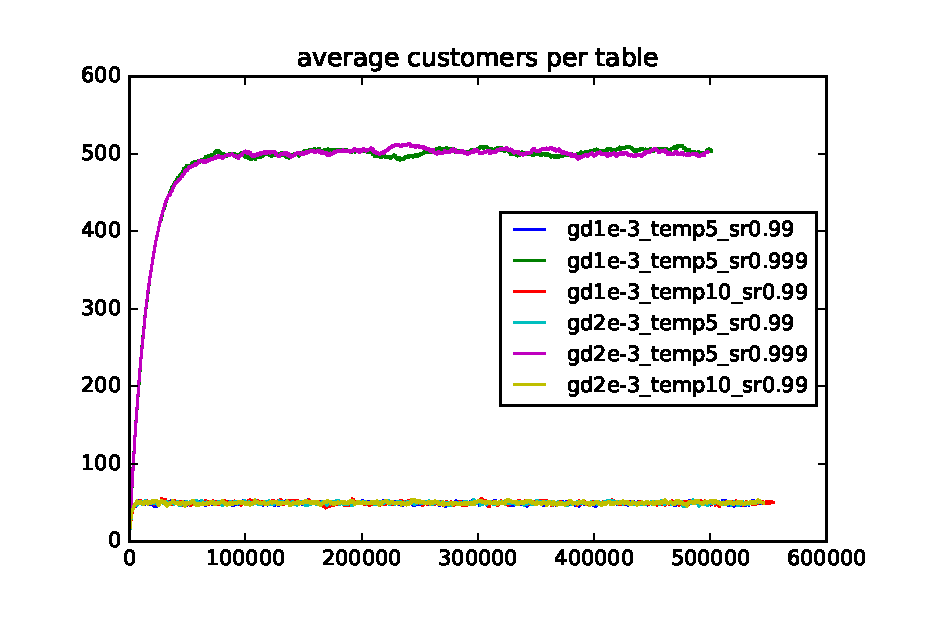
\includegraphics[width = \textwidth]{plans/eps/0_1_2_3_4_5_cnum_avg.eps}
    \caption{}
    \label{fig::plans_a}
  \end{subfigure}
  \begin{subfigure}{0.49\textwidth}
    \centering
    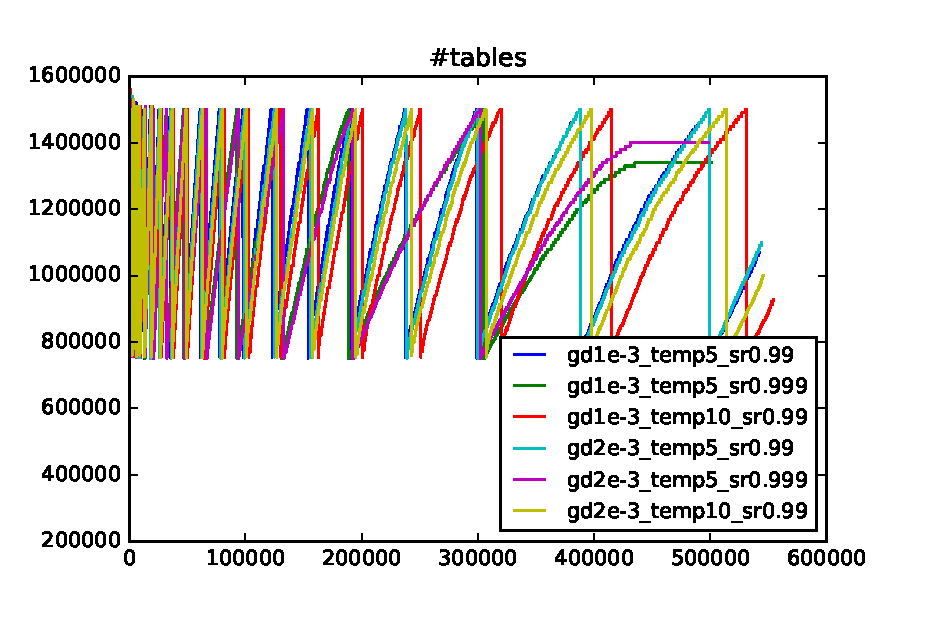
\includegraphics[width = \textwidth]{plans/eps/0_1_2_3_4_5_rest_num.eps}
    \caption{}
    \label{fig::plans_b}
  \end{subfigure}
  \\
  \begin{subfigure}{0.49\textwidth}
    \centering
    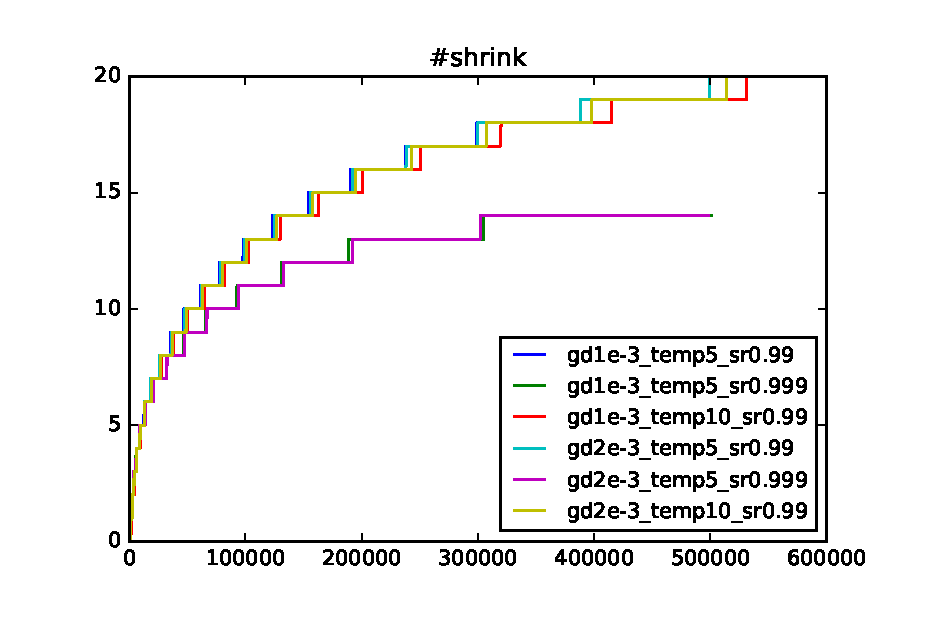
\includegraphics[width = \textwidth]{plans/eps/0_1_2_3_4_5_reduce_cnt.eps}
    \caption{}
    \label{fig::plans_c}
  \end{subfigure}
  \begin{subfigure}{0.49\textwidth}
    \centering
    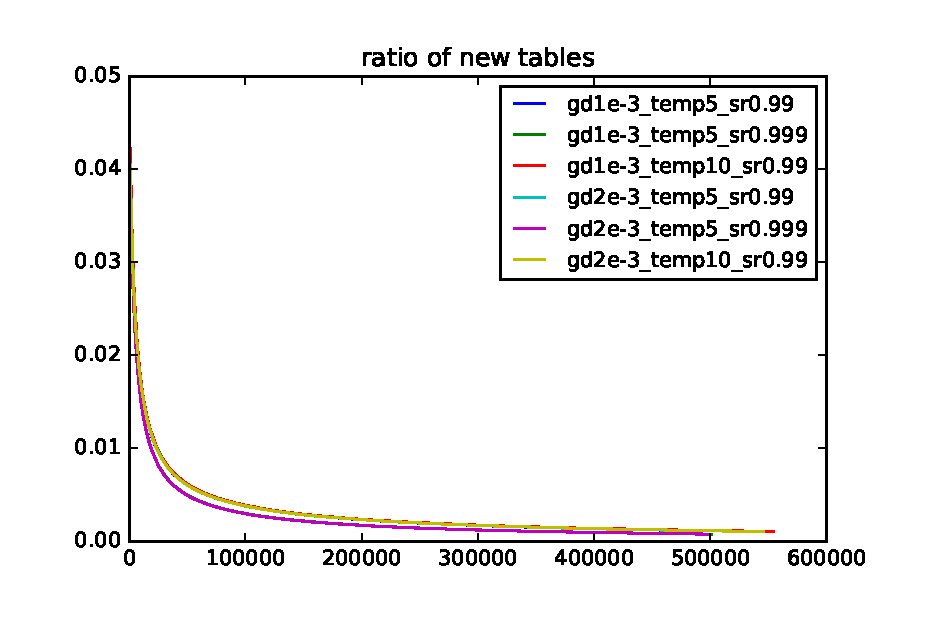
\includegraphics[width = \textwidth]{plans/eps/0_1_2_3_4_5_miss.eps}
    \caption{}
    \label{fig::plans_d}
  \end{subfigure}
  \caption{Curves of average customers per table, number of tables, the number
    of days when tables are pruned, and ratio of customers being assigned to a new
  table. The x-axis is the total number of customers so far. }
  \label{fig::plans}
\end{figure}

To this end, we specifically plot the curves of average customers per table, the
number of tables, the number of days when tables are pruned, and the ratio
between the number of customers being assigned to a new table and all customers.
In Figure~\ref{fig::plans}, the X-axis is the number of customers entering the
restaurant so far. With 48 threads, it was found that appropriate gradient
descent step size ranges from \SI{5e-4} to \SI{4e-3}. Useful final temperature
is from $0.1$ to $0.5$ and the shrink rate $\beta$ from $0.95$ to $0.999$.

Note that the in the curve \ref{fig::plans_a}, $\beta$ is the most influencing
factor. With a larger $\beta = 0.999$, fewer customers are leaving the restaurant
per day. This also contributes to the fact that the tCRP will explore fewer new
tables than with a smaller $\beta = 0.99$, as seen in Figure~\ref{fig::plans_d};
we see a smaller ratio of customers is assigned to new tables. In addition, from
Figure~\ref{fig::plans_c}, we observe that both a larger $\beta$ or a smaller
final temperature can yield fewer number of table pruning. To see this,  note
that with a small final temperature, the stochasticity of PLANS is reduced
exponentially.

\subsection{Classification Experiment}

In this part, we will use the learnt embedding of phrase to represent documents
and see if that can benefit text classification. It was previously shown that by
combining low-dimensional embedding with bag-of-words representation, the
performance can be improved.

We use a classic sentiment classification dataset~\cite{pang2002thumbs}, which
has a set of 700 positive and 700 negative processed movie reviews collected
from the IMDB archive. The dataset is tokenized and words are normalized
already. We followed the use of the data by dividing it into three equal-sized
folds, maintaining balanced class distribution in each fold.  All results
reported below are the average of three-fold cross-validation evaluation on the
dataset.  We use the Logistic-Regression in Scikit-Learn
package~\cite{scikit-learn} for the binary (positive/negative) polarity
classification with different representation strategies for the review
documents.

\begin{table}[h]
  \centering
  \begin{tabular}{c|c|c|c|c|c}
    & Sparse Features & Sparse Dim & Dense Features & Dense Dim & Accuracy \\
    \hline \hline
    (1) & Unigram     & 31,240 & \emph{N.A}  & 0   & 67.512 \\
    (2) & \emph{N.A}  & 0      & Word        & 100 & 58.471 \\
    (3) & \emph{N.A}  & 0      & Phrase      & 100 & 60.332 \\
    (4) & Unigram     & 31,240 & Word        & 100 & 73.637 \\
    (5) & Unigram     & 31,240 & Phrase      & 100 & 77.952 \\ \hline \hline
  \end{tabular}
  \caption{Average three-fold cross-validation accuracies, in percent.}
  \label{tab::plans_cls}
\end{table}

In the experiment, we find $31,240$ unique terms in the reviews. However, note
not all of those words are the top 0.1M frequent words in the NY Times corpus
and it might not always true that there is an embedding vector for each word in
the reviews. From the above Table~\ref{tab::plans_cls}, we see that with the
sparse feature (unigram) only, the baseline performance is merely $67.512\%$.
The unigram baseline is better than only using dense embedding as features.  We
offer two reasons to explain this result: 1) Some discriminative words for
sentiment polarity in the dataset might not has an embedding learnt from the NY
Times and therefore information of those words is lost in the embedding
representation; and 2) The dimension of dense embeddings is only 100 while the
sparse feature has a dimension of $31,240$. Thus models learnt with only dense
embeddings is limited in its capacity to fit the training data and it is
expected that the performance is worse than (1). Comparing (2) and (3), it is
seen that with phrase embeddings learnt from PLANS, there is still a marginal
improvement in performance.

Nevertheless, when combining sparse unigram and dense embedding together, we
observe the best performances. The accuracy for ``unigram+word'' (4) is $73.637$
while the accuracy reaches $77.952$ for ``unigram+phrase'' (5). It is clear that
phrase embeddings learnt by PLANS significantly boost the performance for
polarity classification than that of word embedding. This is also consistent
with the finding by \cite{pang2002thumbs} that bigrams can also benefit the
sentiment classification.


\section{Conclusion}

We propose a novel model, \PLANS{}~(PLANS), to jointly learn the phrasal
allocation and the embeddings. Although previous study have separately
investigated either of the subtasks, PLANS is the first to
address the two problems in a fully unsupervised fashion. PLANS has three main
ingredients: 1). A transient Chinese Restaurant Process (tCRP) is proposed to
model possibly infinite discrete observations in a stream while maintaining an
economic and affordable size of tables and customers by periodical shrinking;
2). Negative sampling~(NS) is integrated to efficiently estimate the
embedding of phrases; and 3). Simulated Annealing~(SA) with geometric cooling
stabilizes PLANS by reducing the stochastic behavior towards the end of
training. In addition, we implement PLANS with multi-threads with a modified
Hogwild algorithm which ensures fast training. Empirical studies demonstrate
that PLANS is able to identify meaningful phrases and accurately estimate the semantic
embeddings.


\chapter{Conclusions}

In this thesis, I describe a range of practical real-world applications where
latent variables can be leveraged for effective knowledge discovery and
efficient optimization. I designed novel probabilistic latent variable models
which manage to model complex distributions through appropriate choices of the
latent variables.

Firstly, I demonstrated that by modeling literature citations as observations of
a generative model with latent variables, research topics as well as evolution
themes of research can be identified and described inactively. The proposed
model 1) discovers research topics, which includes finding milestone papers,
computing topic temporal strength, and extracting keywords for topics; and 2)
identifies research theme evolution, which includes identifying topic
importance, learning topic dependency relation, and recognizing the evolution
patterns. These computational components together enable us to understand
evolution of research themes by constructing the evolution graph.  This work can
be very useful to help researchers digest literature quickly, thus speeding up
scientific research discovery and delivering very broad positive impact on the
society. In general, the model can also be applied to any graph data for tasks
such as network clustering and ranking, as well as modeling the evolution of
network generation.


Secondly, I proposed a framework where a ranked list can be inferred from
pairwise preferences labelled by non-expert workers in crowdsourcing, which is
highly useful in various data mining and information retrieval tasks such as
learning to rank. Latent variables are introduced to model query difficulty and
query domain, as well as worker expertise and truthfulness, effectively
resolving the inevitable incompleteness and inconsistency of pairwise
judgements. In addition, by employing latent variables, intractable
distributions are effectively sampled, and thus efficient computation is
accomplished.

Thirdly, I proposed a novel approach, Dual-Clustering Maximum Entropy, which
addresses the stability problem of Maximum Entropy when there is an extreme
large number of items (classes/words) present. Latent variables are employed for
model reduction and facilitate inference. By incorporating the modeling of
latent variables, the dual space of the Maximum Entropy problem is explored and
a K-means like clustering is conducted over the simplex space. The use of PLVM
leads to an efficient algorithm, the complexity of which does not depend on the
number of items.

In the end, we propose a novel model, Phrasal Latent Allocation with Negative
Sampling (PLANS), to jointly learn the phrasal allocation and the embeddings.
PLANS consists of three key components: 1) A transient Chinese Restaurant
Process (tCRP) is proposed to model possibly infinite discrete observations in a
stream while maintaining an economic and affordable size of tables and customers
by periodical shrinking; 2) Negative sampling~(NS) is integrated to efficiently
estimate the embedding of phrases; and 3) Simulated Annealing~(SA) with
geometric cooling stabilizes PLANS by reducing the stochastic behavior towards
the end of training.  By fitting the unstructured text with underlying phrasal
structures, it is demonstrated that both the phrasal allocation and phrase
embeddings are effectively computed.

Overall, in this thesis, we have explored a wide range of applications where
Probabilistic Latent Variable Models~(PLVMs) can efficiently model data of
different types or greatly improve the performance in terms of efficiency and
scalability. Specifically, we show in this thesis that:

\begin{itemize}
\item PLVMs are a very flexible approach for modeling complex observations (such
  as networks, ranked lists, or sequences) by incorporating latent variables
  into the generative modeling.
\item PLVMs are a powerful tool for knowledge discovery and data mining. By
  encoding the useful information as latent variables and modeling them with
  feasible generative process, it can significatnly simplify the computation and
  achieves good performance.
\item PLVMs can also be leveraged for efficient and salable optimization. As one
  example shown in the thesis, posterior sampling can be leveraged as E-step in
  the E-M algorithm.
\end{itemize}

It is our expectation that PLVMs benefit many other research topics in machine
learning and data mining. The general methodology is that PLVMs allow us to
model complex observations by assuming simpler generation at the cost of
incorporating latent variables into modeling. More importantly, those
``artificially'' added latent variables are in fact statistically meaningful in
most applications, as they preserve crucial information of the data.  In
addition, another merit of PLVMs is that it provides a principle means to
develop scalable and efficient algorithms for inference.  It would be useful to
explore other applications of PLVMs that could benefit from the idea of modeling
with latent variables in the future.


% We conclude that graduate students like coffee.

\bibliographystyle{abbrvnat}
\bibliography{refs}

\appendix
\chapter{Supplementary results on Thurstonian Pairwise Preference}
\section{Model Updating} \label{app::mmu}%M-step

By zeroing  the derivatives of $\mathcal{Q}(\mathbf{\Theta}^{(t+1)};
\mathbf{\Theta}^{(t)})$ with respect to $\mathbf{\Theta}^{(t+1)}$, the following
closed forms are obtained for the update of $\{s_{l,i}^{(t+1)}\}$,
$\{\delta_{l}^{2(t+1)}\}$ and $\{\theta_m^{(t+1)}\}$:

\begin{empheq}[left=\empheqlbrace]{align}
s_{l^*,i^*}^{(t+1)} &=
  \frac{ \sum\limits_{k \in \mathcal{W}_{l^*,i^*}}
    \E_{\mathbf{Z|D,\Theta}^{(t)}}[s_{l^*,i^*}^{(k)}]}
    {\sum\limits_{k \in \mathcal{W}_{l^*,i^*}} 1} \label{eq::mu_ps}\\
\delta_{l^*}^{2(t+1)} &=
  \frac{ \sum\limits_{(k,i) \in \mathcal{P}_{l^*}}
    \E_{\mathbf{Z|D,\Theta}^{(t)}}[(s_{l^*,i}^{(k)} - s_{l^*,i}^{(t+1)})^2] }
    {\sum\limits_{(k,i) \in \mathcal{P}_{l^*}} 1} \label{eq::mu_d}\\
\theta_{m^*}^{(t+1)} &\propto
  \sum\limits_l \E_{\mathbf{Z|D,\Theta}^{(t)}}[\mathbf{1}(m_l = m^*)]
\end{empheq}

where $\mathcal{W}_{l^*,i^*}$  denotes the set of workers who have judged
$d_{i^*}$ for $q_{l^*}$, and $\mathcal{P}_{l^*}$ denotes the set of
$\langle\mbox{worker, document}\rangle$ pairs involved in the annotation for
$q_{l^*}$, \ie,

\begin{align}
\mathcal{W}_{l^*,i^*} &= \{ k ~|~ \exists i, ~ \langle k, l^*,i^*, i \rangle
  \in \mathbf{D} ~\mathrm{or}~\langle k, l^*, i, i^* \rangle \in \mathbf{D}\}
  \nonumber \\
\mathcal{P}_{l^*} &= \{ (k, i) ~|~ \exists \tilde{i},~
  \langle k, l^*,i, \tilde{i} \rangle \in \mathbf{D}
  ~\mathrm{or}~\langle k, l^*, \tilde{i}, i \rangle \in \mathbf{D}\} \nonumber
\end{align}

Unfortunately, $\{\tau_{k,m}^{(t+1)}\}$ do not have a closed-form analytic
solution, where we employ Newton's method.  The partial derivatives
\emph{w.r.t.}  $\tau_{k^*,m^*}^{(t+1)}$ are given by:

\begin{align}
\frac{\partial \mathcal{Q}}{\partial \tau_{k^*,m^*}^{(t+1)}} =
& \sum\limits_{\substack{l, i_1, i_2 \\ \langle k^*, l,i_1,i_2 \rangle
      \in \mathbf{D}}}
  \E_{\mathbf{Z|D,\Theta}^{(t)}}
  \left[ \mathbf{1}(m_l=m^*) \frac{s_{l,i_1}^{(k^*)} -
    s_{l,i_2}^{(k^*)}}{\sqrt{2}} \right. \nonumber \\
&  \left. f\big(-\frac{\tau_{k^*,m^*}^{(t+1)}}{\sqrt{2}}(s_{l,i_1}^{(k^*)} -
    s_{l,i_2}^{(k^*)})\big) \right] \label{eq::tau1}\\
\frac{\partial^2 \mathcal{Q}}{\partial {\tau_{k^*,m^*}^{(t+1)}}^2} =
& -\sum\limits_{\substack{l, i_1, i_2 \\ \langle k^*, l,i_1,i_2 \rangle
    \in \mathbf{D}}}
    \hspace{-15pt}\E_{\mathbf{Z|D,\Theta}^{(t)}}
    \hspace{-2pt}\Bigg[\mathbf{1}(m_l=m^*)
      \frac{(s_{l,i_1}^{(k^*)} - s_{l,i_2}^{(k^*)})^2}{2}  \nonumber \\
& \Big\{ f\big(-\frac{\tau_{k^*,m^*}^{(t+1)}}{\sqrt{2}}(s_{l,i_1}^{(k^*)}
              - s_{l,i_2}^{(k^*)})\big)
        \frac{\tau_{k^*,m^*}^{(t+1)}}{\sqrt{2}}
        (s_{l,i_1}^{(k^*)} - s_{l,i_2}^{(k^*)}) \nonumber \\
&  + f^2 \big(-\frac{\tau_{k^*,m^*}^{(t+1)}}{\sqrt{2}}
        (s_{l,i_1}^{(k^*)} - s_{l,i_2}^{(k^*)})\big)
  \Big\} \Bigg] \label{eq::tau2}
\end{align}

where we used the fact that
$$\partial \mathrm{Q}(x) / \partial x = - \P_\mathtt{N}(x | 0, 1)$$
And $f(\cdot)$ is defined as

\begin{equation}
f(x)=\frac{\P_\mathtt{N}(x | 0,1)}{\mathrm{Q}(x)} \label{eq::f_def}
\end{equation}

whose derivative is calculated as:

\begin{equation}
\frac{\d f(x)}{\d x}  = -x f(x) + f^2(x)
\end{equation}

An important implementation issue of Newton's method is numeric stability.
For large $x > 0$, computing $f(x)$ using \Cref{eq::f_def} is not advised as
both $\P_\mathtt{N}(x | 0, 1)$ and $\mathrm{Q}(x)$ approach zero fast. To
address this issue, we use the following approximation~\cite{chiani2003new}:

\begin{equation}
\mathrm{Q}(x) \approx
  \frac{1}{12}e^{-\frac{x^2}{2}} + \frac{1}{4}e^{-\frac{2}{3}x^2}
\end{equation}

Using this result, $f(x) \approx \frac{12}{\sqrt{2\pi}}$ can be found to be a
good approximation for $x > 8$.

\section{Inference of \textsc{Trm}} \label{app::trm}

\trm{} is the building block of the proposed \tpp{} and is investigated as a
baseline in the experiment. We present the maximum likelihood estimation~(MLE)
using the Expectation-Maximization~(E-M) algorithm.

The joint likelihood is given by

\begin{align}
& \P\big(\{\sigma_l^{(k)}\}, \{s_{l,i}^{(k)}\} |
    \{s_{l,i}\}, \{\delta_l^2\}\big)  \nonumber \\
=
& \prod_{l,i,k} \P_N(s_{l,i}^{(k)} | s_{l,i}, \delta_l^2) \cdot
  \mathds{1}(\sigma_l^{(k)}, \{s_{l,i}^{(k)} \})
\end{align}

where $\mathds{1}(\sigma_l^{(k)}, \{s_{l,i}^{(k)} \}) = 1$ if the ranking
derived from the order of $\{s_{l,i}^{(k)} \}$ is consistent with
$\sigma_l^{(k)}$ and $0$ otherwise.

In addition, like \textsc{Tpp}, the posterior distribution is approximated by
Gibbs sampling,

\begin{align}
& \P\big( s_{l^*,i^*}^{(k^*)} | \{s_{l,i}\}, \{\delta_l^2\}, \{\sigma_l^{(k)}\},
            \{s_{l,i}^{(k)}\} \ \{s_{l^*,i^*}^{(k^*)}\} \big)  \nonumber \\
=
& \P_N(s_{l^*,i^*}^{(k^*)} | s_{l^*,i^*}, \delta_{l^*}^2) \cdot
            \mathds{1}(s_{-} \leq s_{l^*,i^*}^{(k^*)} \leq s_{+} \})
\end{align}

where $s_{+}$ (or $s_{-}$) denotes the worker's perceived score
$s_{l^*,i}^{(k^*)}$ of the document $d_i$ which immediately precedes (or
follows) $d_{i^*}$ as ranked by $\sigma_{l^*}^{(k^*)}$ if such $d_i$ exists or
otherwise evaluated as $+\infty$ (or $-\infty$). Consequently, we samples
$s_{l^*,i^*}^{(k^*)}$ by

$$s_{l^*,i^*}^{(k^*)} \sim \mathrm{TN}_{s_{-}}^{s_{+}}
(s_{l^*,i^*}, \delta_{l^*}^2)$$

Lastly, we update the parameters by optimizing the expected joint log
likelihood, which yields the same updating rules as in \Cref{eq::mu_ps},
\Cref{eq::mu_d} with the only difference being that $k$ is ranged over all
workers that rank for $q_{l^*}$ in \Cref{eq::mu_ps} and $(k,i)$ over all workers
that judge $q_{l^*}$ and documents in the ranking list of $q_{l^*}$ in
\Cref{eq::mu_d}.

A final note of \textsc{Trm} is about its identifiability: It requires rescaling
in the same manner as in \Cref{eq::tpp_id1} and \Cref{eq::tpp_id2} to cancel
extra freedom in order to prevent the model from undesired drifting and scaling.

% \include{Appendix.tex}

\backmatter
% \chapter{Vita}


\end{document}
\endinput
%%
%% End of file `thesis-ex.tex'.
